% ============================================================================
% PONTIFICIA UNIVERSIDAD JAVERIANA
% FACULTAD DE INGENIERIA - SISTEMAS
% Observatorio de Demanda Laboral en América Latina
% ============================================================================

\documentclass[12pt,oneside,letterpaper]{report}

% ============================================================================
% PAQUETES
% ============================================================================
\usepackage[utf8]{inputenc}
\usepackage[spanish,es-tabla]{babel}
\usepackage[letterpaper,top=3cm,bottom=3cm,left=3cm,right=3cm]{geometry}
\usepackage{times}
\usepackage{graphicx}
\usepackage{amsmath,amssymb}
\usepackage{setspace}
\usepackage{fancyhdr}
\usepackage{titlesec}
\usepackage{tocloft}
\usepackage[hidelinks]{hyperref}
\usepackage{listings}
\usepackage{xcolor}
\usepackage{float}
\usepackage{longtable}
\usepackage{multirow}
\usepackage{array}
\usepackage[backend=biber,style=apa,natbib=true]{biblatex}

% TikZ para diagramas
\usepackage{tikz}
\usetikzlibrary{shapes.geometric, arrows.meta, positioning, shadows, fit, shapes.multipart}

% ============================================================================
% CONFIGURACIÓN DE BIBLIOGRAFÍA
% ============================================================================
\addbibresource{bibliografia.bib}

% ============================================================================
% CONFIGURACIÓN DE CÓDIGO
% ============================================================================
\lstset{
    basicstyle=\ttfamily\small,
    breaklines=true,
    frame=single,
    numbers=left,
    numberstyle=\tiny\color{gray},
    keywordstyle=\color{blue},
    commentstyle=\color{green!60!black},
    stringstyle=\color{orange},
    showstringspaces=false
}

% ============================================================================
% CONFIGURACIÓN DE INTERLINEADO
% ============================================================================
\onehalfspacing

% ============================================================================
% CONFIGURACIÓN DE ENCABEZADOS Y PIE DE PÁGINA
% ============================================================================
\pagestyle{fancy}
\fancyhf{}
\fancyhead[L]{Pontificia Universidad Javeriana}
\fancyhead[R]{Undergraduate Final Project Report}
\fancyfoot[R]{Page \thepage}
\renewcommand{\headrulewidth}{0.4pt}
\renewcommand{\footrulewidth}{0.4pt}

% ============================================================================
% CONFIGURACIÓN DE TÍTULOS DE CAPÍTULOS
% ============================================================================
\titleformat{\chapter}[display]
{\normalfont\huge\bfseries\centering}
{\chaptertitlename\ \thechapter}{20pt}{\Huge}

\titleformat{\section}
{\normalfont\Large\bfseries}{\thesection}{1em}{}

\titleformat{\subsection}
{\normalfont\large\bfseries}{\thesubsection}{1em}{}

% ============================================================================
% INFORMACIÓN DEL PROYECTO
% ============================================================================
\newcommand{\proyectoTitulo}{Observatorio de demanda laboral en América Latina}
\newcommand{\proyectoCodigo}{<CODE>}
\newcommand{\autorUno}{Nicolas Francisco Camacho Alarcón}
\newcommand{\autorDos}{Alejandro Pinzón Fajardo}
\newcommand{\director}{Ing. Luis Gabriel Moreno Sandoval}
\newcommand{\juradoUno}{Ing. <Name of the jury>}
\newcommand{\juradoDos}{Ing. <Name of the jury>}
\newcommand{\anio}{2025}
\newcommand{\mes}{<Month>}

% ============================================================================
% DOCUMENTO
% ============================================================================
\begin{document}

% Páginas preliminares sin numeración
\pagenumbering{gobble}

% Portada principal
% ============================================================================
% PORTADA - SRS
% Especificación de Requerimientos de Software
% ============================================================================

\begin{titlepage}
\centering

\vspace*{1cm}

{\Large\bfseries \proyectoTitulo\par}
\vspace{0.5cm}
{[Grupo 8]\par}

\vspace{2cm}

{\Large\bfseries ESPECIFICACIÓN DE REQUERIMIENTOS DE SOFTWARE\par}

\vspace{1cm}

{[\fecha]\par}
\vspace{0.5cm}


\vspace{2cm}

\includegraphics[width=0.4\textwidth]{logo-javeriana.png}

\vfill

{\large Autores:\par}
\vspace{0.5cm}
{\large \autorUno\par}
{\large \autorDos\par}

\vspace{1cm}

{\large Pontificia Universidad Javeriana\par}
{\large Facultad de Ingeniería\par}
{\large Bogotá, Colombia\par}
{\large \mes{} de \anio\par}

\end{titlepage}

\newpage

% Página en blanco
\thispagestyle{empty}
\mbox{}
\newpage

% Portada interna
\thispagestyle{fancy}

\begin{center}
    {\large\bfseries \proyectoCodigo\par}
    \vspace{0.5cm}
    {\large\bfseries \proyectoTitulo\par}
\end{center}

\vspace{2cm}

\begin{center}
    {\large\bfseries Autor(es):\par}
    \vspace{0.5cm}
    {\large \autorUno\par}
    {\large \autorDos\par}
\end{center}

\vspace{2cm}

\begin{center}
    MEMORIA DE PROYECTO DE GRADO REALIZADO PARA CUMPLIR UNO DE LOS REQUISITOS PARA EL TÍTULO EN INGENIERÍA DE SISTEMAS
\end{center}

\vspace{1.5cm}

\begin{center}
    {\large\bfseries Director\par}
    \vspace{0.5cm}
    {\large \director\par}

    \vspace{1cm}

    {\large\bfseries Jurados del Proyecto de Grado\par}
    \vspace{0.5cm}
    {\large \juradoUno\par}
    {\large \juradoDos\par}
\end{center}

\vspace{1.5cm}

\begin{center}
    {\large PONTIFICIA UNIVERSIDAD JAVERIANA\par}
    {\large FACULTAD DE INGENIERÍA\par}
    {\large CARRERA DE INGENIERÍA DE SISTEMAS\par}
    {\large BOGOTÁ, D.C.\par}
    {\large \mes, \anio\par}
\end{center}

\newpage

% Página en blanco
\thispagestyle{empty}
\mbox{}
\newpage

% Autoridades
\thispagestyle{fancy}

\begin{center}
    {\large\bfseries PONTIFICIA UNIVERSIDAD JAVERIANA\par}
    {\large\bfseries FACULTAD DE INGENIERIA\par}
    {\large\bfseries SYSTEMS ENGINEERING PROGRAM\par}
\end{center}

\vspace{4cm}

\begin{center}
    {\large\bfseries President of the Pontificia Universidad Javeriana\par}
    \vspace{0.5cm}
    {\large <Name of the President of the University>\par}

    \vspace{2cm}

    {\large\bfseries Dean of School of Engineering\par}
    \vspace{0.5cm}
    {\large <Name of the Dean>\par}

    \vspace{2cm}

    {\large\bfseries Head of the Systems Engineering Program\par}
    \vspace{0.5cm}
    {\large <Name of the head of the program>\par}

    \vspace{2cm}

    {\large\bfseries Head of the Systems Engineering Department\par}
    \vspace{0.5cm}
    {\large <Name of the head of the department>\par}
\end{center}

\newpage

% Artículo 23
\thispagestyle{fancy}

{\large\bfseries Artículo 23 de la Resolución No. 1 de Junio de 1946}

\vspace{1cm}

\textit{``La Universidad no se hace responsable de los conceptos emitidos por sus alumnos en sus proyectos de grado. Sólo velará porque no se publique nada contrario al dogma y la moral católica y porque no contengan ataques o polémicas puramente personales. Antes bien, que se vean en ellos el anhelo de buscar la verdad y la Justicia''}

\newpage

% Agradecimientos
\thispagestyle{fancy}

\begin{center}
    {\large\bfseries AGRADECIMIENTOS}
\end{center}

\vspace{1cm}

\noindent\textbf{Nicolás Francisco Camacho Alarcón}

\vspace{0.5cm}

Llegar hasta aquí ha sido un camino largo y sinuoso, lleno de dudas, decisiones difíciles y momentos en los que pensé que no podría seguir adelante. Tras un camino de búsqueda que me llevó por tres carreras diferentes y siete años de aprendizaje constante, hoy puedo decir que cada paso, cada tropiezo y cada nueva dirección me trajeron exactamente donde debía estar.

En primer lugar, quiero agradecer a mis padres, quienes desde pequeño me impulsaron a crecer académicamente, a alcanzar nuevas metas y a nunca conformarme. Gracias por apoyarme en cada cambio de rumbo, por entender mis búsquedas y por nunca dejar de creer en mí, incluso cuando yo mismo dudaba. Su amor y esfuerzo constante han sido el pilar que me sostuvo en los momentos más difíciles. A mi hermana, mi apoyo incondicional y prácticamente mi mejor amiga, gracias por estar siempre ahí, por escucharme, por animarme y por ser esa compañía invaluable en cada etapa de este proceso. A mi abuela, por su cariño y por ser parte fundamental de esta familia que me ha dado todo. A toda mi familia, gracias por comprenderme, por acompañarme en cada gran decisión, por ayudarme a levantarme cuando sentí que no podía más, y por estar presentes en cada momento importante de mi vida.

Un agradecimiento muy especial a Lucy, mi perrita, quien con su compañía silenciosa y su alegría incondicional trajo luz a cada día, sin importar lo difícil que fuera. Su presencia fue un refugio de paz y felicidad en medio de las noches largas y los momentos de mayor estrés.

A todos los amigos que he ido conociendo semestre a semestre desde que entré a primer semestre de música, pasando por electrónica y llegando a sistemas: gracias por hacer de estos años una experiencia llena de aprendizajes, risas y compañía. Cada uno de ustedes aportó algo valioso a mi camino y me ayudó a convertirme en quien soy hoy.

A todos mis profesores, gracias por inspirarme semestre tras semestre a ser mejor, a alcanzar nuevos niveles y a recordarme constantemente que amo aprender y que me apasiona sentirme retado. Su dedicación y enseñanzas fueron fundamentales para mantener viva esa chispa de curiosidad que me impulsa.

A Alejandro, mi compañero de tesis, gracias por haberme acompañado este año y por haber sido el apoyo que necesité en el tramo final para lograrlo. Tu paciencia y tu apoyo emocional fueron invaluables, y estoy profundamente agradecido por haber compartido este proceso contigo.

A Gabriel, nuestro director de tesis, por inspirarnos y ayudarnos a encontrar algo realmente retador e innovador que nos permitiera hacer algo nuevo en la industria. Tu guía fue clave para que este proyecto tomara forma y alcanzara su verdadero potencial.

A Sezzle, mi empresa, gracias por permitirme terminar mi carrera al tiempo que trabajo, y por apoyarme para salir adelante. Su comprensión y flexibilidad fueron fundamentales para lograr este objetivo.

Finalmente, quiero agradecer a ese Nicolás que decidió levantarse una vez más, por haber tenido la valentía de buscar su verdadero camino y por haber confiado en que encontraría su lugar, incluso cuando el camino no estaba claro. Este logro también es tuyo.

A todos los que han sido parte de este camino: gracias. Este trabajo es el resultado no solo de mi esfuerzo, sino del amor, la paciencia y el acompañamiento de cada uno de ustedes.

\vspace{1cm}

\noindent\textbf{Alejandro Pinzón Fajardo}

\vspace{0.5cm}

La culminación de este trabajo representa mucho más que un logro académico; es el resultado de años de esfuerzo, constancia y del apoyo invaluable de las personas que me han acompañado a lo largo de este camino.

Mi familia ha sido el pilar fundamental de este proceso. Su amor, paciencia y fe inquebrantable me brindaron la fortaleza necesaria para avanzar incluso en los momentos más difíciles. Gracias por enseñarme el valor del trabajo honesto, la disciplina y la perseverancia que hoy hacen posible este resultado.

Durante mi formación en la Pontificia Universidad Javeriana, tuve el privilegio de aprender de profesores que, más allá de impartir conocimiento, despertaron en mí la curiosidad, el pensamiento crítico y la pasión por la ingeniería. Su dedicación y compromiso fueron esenciales para mi crecimiento profesional y personal.

El desarrollo de esta tesis no habría sido posible sin la guía del profesor Gabriel, cuya orientación y criterio fueron determinantes para dar forma y sentido al proyecto. Su apoyo y su exigencia académica nos permitieron alcanzar un resultado del que me siento profundamente orgulloso.

Finalmente, compartir este proceso con Nicolás fue una experiencia gratificante. Su compromiso, su disposición al trabajo en equipo y su acompañamiento hicieron de esta etapa un recorrido más llevadero y enriquecedor, en el que aprendimos tanto del proyecto como de nosotros mismos.

A todos ellos, mi gratitud más sincera.

\newpage

% Tabla de contenidos
\pagenumbering{roman}
\setcounter{page}{6}
\renewcommand{\contentsname}{CONTENT}
\tableofcontents
\newpage

% Abstract
\thispagestyle{fancy}

\begin{center}
    {\large\bfseries RESUMEN}
\end{center}

\vspace{1cm}

El mercado laboral tecnológico latinoamericano carece de sistemas automatizados para caracterizar la demanda de habilidades técnicas IT de manera sistemática y actualizada, enfrentando el desafío de capturar tecnologías emergentes que evolucionan más rápido que taxonomías oficiales. Este proyecto evaluó la viabilidad de construir un observatorio automatizado que recolectó 30,660 ofertas laborales de Colombia, México y Argentina mediante web scraping de siete portales, focalizándose en extracción de hard skills (lenguajes de programación, frameworks, herramientas cloud/DevOps, metodologías ágiles). Se implementó Pipeline A (NER + Regex) procesando el corpus completo con latencia de 0.97s por oferta, y se desarrolló Pipeline B experimental (LLM Gemma 3 4B) evaluado sobre gold standard de 300 ofertas anotadas manualmente con 6,174 hard skills. Los resultados demostraron superioridad de modelos de lenguaje para aproximar mapeo humano de competencias técnicas (F1=84.26\% vs 72.53\%), capturando habilidades implícitas inferibles del contexto y tecnologías emergentes ausentes en vocabularios controlados que métodos basados en patrones omiten. El sistema normalizó extracciones contra taxonomía ESCO v1.1.0 extendida con 276 habilidades técnicas modernas (152 O*NET + 124 curadas manualmente) mediante matcher conservador de dos capas (exacto + difuso threshold 0.92), alcanzando 12.6\% de cobertura. Experimentos con matcher enhanced aumentaron cobertura a ~25\% pero no se implementó en producción para mantener neutralidad entre pipelines, evidenciando que 70-87\% de habilidades detectadas son emergentes no presentes en taxonomías estándar (Next.js, Tailwind CSS, Terraform, Bun), validando necesidad de captura automática de vocabulario IT actual. El clustering no supervisado (UMAP reducción 768D a 2D + HDBSCAN density-based) identificó entre 34 y 53 familias tecnológicas en configuraciones optimizadas, sin categorías predefinidas. Los hallazgos validan tres conclusiones: primero, la viabilidad técnica de observatorios basados en scraping multi-portal; segundo, la superioridad de LLMs versus métodos deterministas para extracción semántica y detección de emergentes, con trade-off de costo computacional hasta 43$\times$ mayor; y por último, la obsolescencia crítica de taxonomías oficiales para vocabulario IT actual, evidenciando necesidad de actualización continua.

\newpage

% Iniciar numeración arábiga para el contenido
\pagenumbering{arabic}

% ============================================================================
% CAPÍTULOS PRINCIPALES
% ============================================================================

\chapter{INTRODUCCIÓN}

\section{Propósito}

El presente documento tiene como propósito especificar de manera detallada los requerimientos funcionales y no funcionales del sistema denominado Observatorio de Demanda Laboral en Tecnología en Latinoamérica, una herramienta de análisis automatizado orientada a procesar, extraer y segmentar habilidades tecnológicas desde portales de empleo en línea, mediante técnicas modernas de procesamiento de lenguaje natural, scraping, embeddings semánticos y clustering no supervisado.

Este documento está dirigido principalmente a tres audiencias complementarias. En primer lugar, sirve como guía estructurada para el equipo de desarrollo del proyecto, compuesto por los estudiantes \autorUno{} y \autorDos{}, orientando la implementación y validación del sistema. En segundo lugar, constituye evidencia formal del entendimiento técnico y conceptual del producto para el director del proyecto, \director{}, y los jurados evaluadores. Finalmente, proporciona un marco de referencia para otros actores académicos o institucionales interesados en replicar o adaptar el sistema en contextos similares, tales como universidades, centros de investigación o entidades públicas vinculadas al análisis del mercado laboral.

El documento cubre la totalidad del sistema propuesto, sin limitarse a un solo módulo o subsistema. Por tanto, especifica requerimientos relacionados con la adquisición de datos mediante scraping, su procesamiento semántico, análisis estadístico y segmentación por perfiles laborales, así como aspectos de validación, modularidad, documentación técnica y estándares de calidad.

La importancia de este documento radica en su papel como contrato técnico entre los actores involucrados, asegurando una visión compartida del comportamiento esperado del sistema, las restricciones existentes, los criterios de aceptación y los estándares metodológicos adoptados. Además, facilita la trazabilidad entre los objetivos definidos en la propuesta de grado y las funcionalidades implementadas en cada fase, garantizando coherencia metodológica, control de calidad y sostenibilidad del desarrollo.

\section{Alcance}

El sistema propuesto, titulado Observatorio de Demanda Laboral en Tecnología en Latinoamérica, tiene como propósito desarrollar una herramienta automatizada capaz de analizar la evolución de las habilidades tecnológicas demandadas en el mercado laboral digital, específicamente en los países de Colombia (CO), México (MX) y Argentina (AR). El sistema abarca desde la recolección periódica de datos a través de scraping en portales de empleo hasta el procesamiento semántico y la segmentación de perfiles laborales utilizando técnicas avanzadas de NLP y clustering no supervisado.

El alcance geográfico del observatorio comprende tres países latinoamericanos: Colombia, México y Argentina. Las fuentes de datos corresponden a 7 portales de empleo principales que concentran la mayor parte de las ofertas laborales tecnológicas en la región, incluyendo Computrabajo, Bumeran, ElEmpleo, HiringCafe, OCC Mundial, ZonaJobs e Indeed.

La taxonomía base del sistema constituye una integración unificada de 14,174 habilidades, compuesta por 13,939 competencias de la base europea ESCO v1.1.0, complementadas con 152 tecnologías emergentes del catálogo O*NET Hot Technologies del sector IT, y 83 habilidades curadas manualmente específicas para el mercado tecnológico latinoamericano. El stack tecnológico seleccionado incluye Python 3.10 o superior como lenguaje base, Scrapy para extracción automatizada, spaCy para procesamiento de lenguaje natural, PostgreSQL como sistema de gestión de base de datos, FAISS para búsqueda vectorial eficiente, el modelo de embeddings multilingües E5 de 768 dimensiones, y los algoritmos HDBSCAN y UMAP para clustering y reducción dimensional respectivamente.

El producto incluye siete funcionalidades principales integradas en un pipeline secuencial. La primera funcionalidad corresponde a la extracción automatizada de vacantes desde los portales web mediante spiders especializados que respetan las normas de uso de cada sitio. La segunda funcionalidad implementa preprocesamiento y limpieza textual mediante tokenización, lematización y normalización de formatos, preparando los datos para análisis posterior. La tercera funcionalidad ejecuta la detección de habilidades explícitas e implícitas mediante técnicas híbridas que combinan reconocimiento de entidades nombradas, expresiones regulares y modelos de lenguaje.

La cuarta funcionalidad genera representaciones semánticas mediante el modelo de embeddings E5 de 768 dimensiones, seguido de reducción dimensional con UMAP para visualización y agrupación eficiente. La quinta funcionalidad mapea las habilidades extraídas contra la taxonomía ESCO mediante una estrategia de tres capas que incluye matching exacto, fuzzy matching con umbral de similitud del 85 por ciento, y semantic matching mediante búsqueda vectorial con FAISS. La sexta funcionalidad agrupa perfiles laborales mediante el algoritmo HDBSCAN, que permite segmentar la demanda en grupos funcionales coherentes sin requerir especificación previa del número de clusters. La séptima funcionalidad genera visualizaciones macro mediante gráficos interpretables y reportes estáticos, complementados por un dashboard web interactivo desarrollado con Next.js que permite consulta dinámica de métricas y tendencias. Finalmente, el sistema proporciona documentación metodológica completa y código reproducible que permite replicar o adaptar la solución a otras regiones o sectores bajo principios de ética, apertura científica y eficiencia computacional.

El alcance funcional se circunscribe al dominio de las ofertas de empleo tecnológicas publicadas en español en los países mencionados, sin contemplar vacantes en otros idiomas ni otros sectores económicos. Sin embargo, el diseño modular del sistema permitirá su adaptación futura a nuevos contextos geográficos o temáticos.

\section{Definiciones, Acrónimos y Abreviaciones}

\subsection{Portales de empleo}
Son plataformas web donde empresas publican vacantes laborales y profesionales buscan oportunidades. En este proyecto se consideran fuentes como LinkedIn, Computrabajo, Bumeran, ZonaJobs e Indeed, que constituyen insumos primarios para los procesos de scraping y análisis \cite{aguilera2018, cardenas2015}.

\subsection{Web Scraping}
Técnica de recolección automatizada de datos desde páginas web, utilizando librerías como BeautifulSoup, Selenium o Playwright. Permite extraer de forma estructurada información relevante de las ofertas publicadas \cite{orozco2019}.

\subsection{Oferta laboral}
Se refiere al anuncio publicado por una organización donde se describe el perfil buscado, incluyendo título del cargo, funciones, requisitos y habilidades deseadas \cite{rubio2024}.

\subsection{Base de datos relacional (PostgreSQL)}
Sistema que organiza los datos recolectados en tablas interconectadas, facilitando su consulta, limpieza y posterior análisis mediante estructuras SQL \cite{martinez2024}.

\subsection{Normalización de datos}
Proceso de limpieza, estandarización y unificación de formatos para reducir ambigüedad, errores y duplicados, y mejorar la coherencia del análisis posterior \cite{martinez2024}.

\subsection{Expresiones regulares (Regex)}
Lenguaje sintáctico utilizado para identificar y extraer patrones textuales específicos (como frases que contengan habilidades o requisitos) en grandes volúmenes de texto.

\subsection{Named Entity Recognition (NER)}
Técnica de procesamiento de lenguaje natural (NLP) que identifica y clasifica entidades en un texto, como nombres de habilidades, empresas o tecnologías \cite{vasquez2024, aitoskillner}.

\subsection{Tokenización}
Consiste en dividir un texto en unidades mínimas llamadas ``tokens'' (palabras, signos u oraciones), facilitando el análisis lingüístico automatizado.

\subsection{Lematización}
Proceso que transforma las palabras a su forma canónica o raíz gramatical, permitiendo uniformar variaciones morfológicas del lenguaje.

\subsection{Stopwords}
Términos frecuentes sin valor informativo (como ``de'', ``por'', ``la''), comúnmente eliminados en tareas de procesamiento textual.

\subsection{Co-ocurrencia}
Medida estadística que indica la frecuencia con que dos o más términos aparecen juntos en un texto, útil para detectar relaciones semánticas \cite{lukauskas2023}.

\subsection{Bigramas y trigramas}
Secuencias de dos o tres palabras consecutivas utilizadas para capturar patrones de lenguaje más complejos que las palabras individuales.

\subsection{LLM (Large Language Models)}
Modelos de lenguaje de gran escala (como GPT o T5) entrenados sobre corpus masivos, capaces de generar texto, extraer conocimiento implícito y realizar razonamiento contextualizado \cite{nguyen2024}.

\subsection{Prompt Engineering}
Diseño estratégico de instrucciones o ejemplos para guiar la salida de un LLM, crucial en tareas de extracción de habilidades o clasificación de ocupaciones \cite{nguyen2024}.

\subsection{Few-shot learning}
Habilidad de los LLMs para realizar tareas complejas con pocos ejemplos, lo cual resulta clave cuando se carece de datasets etiquetados masivamente en español \cite{nguyen2024}.

\subsection{Embeddings semánticos}
Representaciones numéricas de textos que capturan similitudes semánticas, permitiendo análisis cuantitativos y clustering. Ejemplos incluyen word2vec, BERT y E5 \cite{kavas2024}.

\subsection{Embeddings multilingües}
Vectores entrenados para representar texto en múltiples idiomas en un mismo espacio semántico. Son esenciales para manejar contenido mixto español-inglés en ofertas laborales \cite{kavas2025}.

\subsection{UMAP (Reducción de dimensionalidad)}
Técnica que transforma espacios de alta dimensionalidad en representaciones más simples, conservando la estructura semántica subyacente para facilitar análisis y visualización.

\subsection{Clustering (HDBSCAN)}
Algoritmo no supervisado que detecta grupos naturales de observaciones (como habilidades o perfiles laborales) según su similitud semántica, sin requerir número de clusters predefinido \cite{lukauskas2023}.

\subsection{Taxonomía de habilidades (ESCO, CIUO-08, O*NET)}
Sistemas jerárquicos y normalizados de clasificación de habilidades y ocupaciones, fundamentales para anclar el análisis a estándares internacionales y mejorar interoperabilidad de los resultados \cite{echeverria2022, campos2024}.

\subsection{FAISS (Facebook AI Similarity Search)}
Biblioteca de código abierto para búsqueda eficiente de similitud en espacios vectoriales de alta dimensionalidad. El sistema utiliza FAISS IndexFlatIP para búsqueda exacta de vecinos más cercanos con producto interno, logrando velocidades de 30,147 consultas por segundo, aproximadamente 25 veces más rápido que PostgreSQL con pgvector.

\subsection{Estrategia de tres capas (Three-layer matching)}
Metodología implementada para mapear habilidades extraídas contra la taxonomía ESCO:
\begin{itemize}
    \item Layer 1 - Exact Match: Búsqueda exacta mediante SQL ILIKE con confianza 1.0
    \item Layer 2 - Fuzzy Match: Similitud difusa con fuzzywuzzy, threshold 0.85, confianza 0.85-1.0
    \item Layer 3 - Semantic Match: Búsqueda semántica con FAISS, threshold 0.87, confianza 0.87-1.0 (actualmente deshabilitado debido a limitaciones del modelo E5 con vocabulario técnico)
\end{itemize}

\subsection{Skills emergentes}
Habilidades extraídas de ofertas laborales que no pueden ser mapeadas a la taxonomía ESCO existente. Representan el 87.4\% de las skills extraídas y constituyen una señal valiosa sobre tendencias emergentes del mercado tech latinoamericano, no un fallo del sistema.

\subsection{Natural Language Processing (NLP)}
Conjunto de técnicas de inteligencia artificial, combinando modelos de lingüística computacional, machine learning y aprendizaje profundo, para poder procesar lenguaje humano.

\subsection{Python}
Lenguaje de programación ampliamente utilizado en ciencia de datos y NLP, por su sintaxis sencilla y librerías especializadas como scikit-learn, spaCy, transformers y pandas.

\section{Apreciación Global}

El presente documento de Especificación de Requerimientos del Software tiene como objetivo presentar de manera estructurada y detallada los aspectos fundamentales del sistema Observatorio de Demanda Laboral en Tecnología en Latinoamérica. La organización del documento se ha realizado con el propósito de facilitar su comprensión tanto para usuarios técnicos como no técnicos, brindando una visión progresiva desde el contexto general hasta los requerimientos específicos del sistema.

El contenido del documento se distribuye en tres secciones principales. La Sección 1 expone la introducción general del proyecto, incluyendo su propósito, alcance, definiciones clave, referencias utilizadas y una apreciación global de su contenido. La Sección 2 describe de manera general los factores que afectan al producto, incluyendo su perspectiva dentro del ecosistema tecnológico, interfaces con otros sistemas y con el usuario, consideraciones de hardware y software, restricciones operativas, y requerimientos de adaptación al entorno de despliegue. La Sección 3 presenta los requerimientos funcionales y no funcionales del sistema, detallando exhaustivamente cada funcionalidad esperada, las restricciones técnicas y operativas, las condiciones necesarias para su correcto funcionamiento, los criterios de validación y verificación, los atributos de calidad del software, los requerimientos de base de datos, la trazabilidad entre objetivos y requerimientos, y el estado actual de implementación de cada módulo del sistema.

Este documento servirá como base para el diseño, desarrollo, validación y evaluación del sistema propuesto, asegurando que todos los actores involucrados compartan una visión clara y consensuada de los objetivos, alcances y funcionalidades del software a implementar. Además, constituye un instrumento de trazabilidad que permite verificar el cumplimiento de cada requerimiento especificado durante el ciclo de vida del proyecto.

% ============================================================================

\chapter{CONTEXTO DEL PROBLEMA}

\section{Oportunidad y problema}

\subsection{Contexto del problema}

El mercado laboral en América Latina se encontró, durante la última década, en una compleja encrucijada definida por la confluencia de dos fuerzas a menudo contrapuestas: una acelerada transformación digital y la persistencia de desafíos estructurales, como una elevada informalidad laboral y brechas de capital humano \cite{echeverria2022}. La pandemia de COVID-19 actuó como un catalizador sin precedentes, intensificando la adopción de tecnologías y, con ello, la demanda de competencias digitales, al tiempo que exponía la vulnerabilidad de los mercados de trabajo de la región \cite{azuara2022}. Este dinamismo generó el riesgo de que la automatización y la digitalización, de no ser gestionadas estratégicamente, pudiesen exacerbar las desigualdades existentes, conduciendo a una mayor polarización y segmentación social \cite{echeverria2022}.

Para analizar este fenómeno regional de manera tangible y robusta, este proyecto seleccionó como casos de estudio a tres de las economías más grandes y digitalmente activas de habla hispana: Colombia, México y Argentina. La elección de estos países respondió a tres criterios estratégicos. Primero, su alto volumen de publicaciones de ofertas laborales en portales digitales aseguró la viabilidad de una recolección masiva de datos (web scraping), fundamental para el entrenamiento de modelos de lenguaje robustos \cite{aguilera2018, martinez2024, rubio2024}. Segundo, la existencia de estudios previos en cada país, aunque metodológicamente limitados, confirmó la pertinencia del problema y proporcionó una línea de base para la comparación \cite{cardenas2015}. Y tercero, su diversidad en términos de realidades económicas, territoriales y de madurez digital permitió validar que la solución desarrollada fuese portable y adaptable a los distintos contextos que caracterizan a América Latina.

\subsection{El caso de Colombia: cambio estructural en la demanda de habilidades}

El caso de Colombia sirvió como una ilustración profunda de esta dinámica. El diagnóstico nacional previo al proyecto ya indicaba que el principal cuello de botella para la inclusión digital no era la falta de infraestructura, sino la brecha de capital humano. Específicamente, el ``Índice de Brecha Digital'' (IBD) del Ministerio de Tecnologías de la Información y las Comunicaciones reveló que la dimensión de ``Habilidades Digitales'' constituía el mayor componente individual de la brecha en el país.

Esta evidencia fue posteriormente corroborada y cuantificada por el análisis empírico de la demanda laboral, el cual demostró que la pandemia generó un cambio estructural y persistente en el mercado. Se encontró que, en los 18 meses posteriores al inicio de la crisis sanitaria, las vacantes tecnológicas aumentaron en un 50\% en comparación con las no tecnológicas \cite{rubio2024}.

Este cambio no fue solo cuantitativo, sino también cualitativo: se observó una marcada caída en la demanda de herramientas ofimáticas tradicionales como Excel (cuya mención en ofertas cayó del 35.8\% en 2018 al 17.4\% en 2023) y un surgimiento exponencial de tecnologías especializadas asociadas al desarrollo web y la gestión de datos, como bases de datos NoSQL (12.3\%), el framework Django (5.5\%) y la librería React (5.3\%) para el año 2023 \cite{rubio2024}.

\subsection{Realidades en México y Argentina}

De manera similar, en México se ha documentado un desajuste significativo entre la oferta educativa y la demanda laboral en el sector tecnológico. El análisis de miles de ofertas laborales reveló que las empresas demandan perfiles con habilidades especializadas en desarrollo de software, análisis de datos y ciberseguridad, mientras que la oferta de graduados se concentra en áreas tradicionales de sistemas \cite{martinez2024}.

En Argentina, el sector de Tecnologías de la Información ha experimentado un crecimiento sostenido, convirtiéndose en uno de los principales generadores de empleo calificado. Sin embargo, la identificación de las tecnologías y roles más demandados ha sido un desafío constante para instituciones educativas y agencias de empleo \cite{aguilera2018}.

\subsection{Formulación del problema}

A pesar de que el contexto del problema ---la creciente e insatisfecha demanda de habilidades tecnológicas--- estaba claramente identificado, los métodos existentes en la región para analizarlo presentaban limitaciones metodológicas significativas que impedían una comprensión profunda y ágil del fenómeno.

Los estudios de referencia en los países seleccionados, si bien valiosos para establecer tendencias macro, se basaron en enfoques de análisis léxico y reglas manuales. En Colombia, el análisis se centró en un sistema de clasificación basado en la Clasificación Internacional Uniforme de Ocupaciones (CIUO), utilizando algoritmos de emparejamiento de texto con tokenización y métricas de similitud basadas en n-gramas \cite{rubio2024}. De forma análoga, en Argentina, los estudios se concentraron en técnicas de minería de texto con análisis de frecuencias y bigramas para identificar patrones en las ofertas del sector TI \cite{aguilera2018}. En México, el enfoque combinó datos de encuestas con scraping de portales, apoyándose en el análisis de frecuencia de términos y la creación de tipologías manuales para segmentar las habilidades \cite{martinez2024}.

La limitación fundamental compartida por estos enfoques es su dependencia de la correspondencia léxica explícita, lo que los hace incapaces de capturar la riqueza semántica del lenguaje. Estos métodos no podían:

\begin{itemize}
    \item Detectar habilidades implícitas (aquellas que se infieren del contexto de un cargo pero no se mencionan directamente)
    \item Gestionar la ambigüedad del lenguaje informal o el uso de anglicismos técnicos (``Spanglish'')
    \item Identificar clústeres de competencias emergentes que aún no forman parte de taxonomías estandarizadas
\end{itemize}

La alta variabilidad en la redacción de las ofertas laborales, la falta de estructuras normalizadas y la rápida aparición de nuevas tecnologías hacían que estos sistemas fueran metodológicamente frágiles y requirieran un constante mantenimiento manual \cite{echeverria2022}.

\subsection{Vacío identificado a nivel institucional}

Más allá de las limitaciones académicas individuales, esta carencia de infraestructura analítica ha sido reconocida a nivel institucional. El Banco Interamericano de Desarrollo (BID) ha señalado la falta de pipelines de análisis modernos y automatizados en la región, destacando que la mayoría de los sistemas existentes, si bien articulan el scraping, todavía se basan en reglas fijas o mapeos manuales y no han incorporado técnicas de embeddings ni de NLP avanzado \cite{echeverria2022}.

En consecuencia, el problema específico que este proyecto abordó fue la ausencia de una herramienta automatizada y de extremo a extremo que, adaptada a las particularidades lingüísticas y estructurales del español latinoamericano, permitiera superar las limitaciones de los análisis léxicos tradicionales. Se identificó la necesidad de un sistema capaz de extraer, estructurar y analizar la evolución de las habilidades tecnológicas de manera semántica, escalable y con un mayor grado de autonomía, integrando para ello técnicas avanzadas de Procesamiento de Lenguaje Natural (NLP), enriquecimiento contextual con Large Language Models (LLMs) y algoritmos de agrupamiento no supervisado.

\section{Propuesta de solución}

Para dar respuesta al problema formulado, se diseñó e implementó un observatorio de demanda laboral tecnológica basado en un pipeline modular y automatizado, un proyecto enmarcado en las áreas de Ingeniería de Sistemas y Ciencia de Datos. El sistema fue concebido como una solución de extremo a extremo que integró las etapas de recolección, procesamiento, análisis semántico y segmentación de ofertas de empleo publicadas en Colombia, México y Argentina. El objetivo fue crear una arquitectura robusta, replicable y adaptada a las complejidades del contexto latinoamericano, superando las limitaciones de los enfoques puramente léxicos o manuales.

La solución se materializó a través de un sistema compuesto por módulos secuenciales y cohesivos. El primer módulo consistió en un motor de adquisición de datos que, mediante técnicas de web scraping, extrajo de forma sistemática y ética decenas de miles de ofertas laborales de portales de empleo clave en la región. El núcleo del sistema fue su arquitectura de extracción dual, compuesta por dos pipelines paralelos:

\textbf{Pipeline A (Tradicional):} Implementó un método de extracción basado en Reconocimiento de Entidades Nombradas (NER) utilizando un EntityRuler de spaCy, poblado con la taxonomía completa de ESCO, combinado con expresiones regulares para capturar un baseline de habilidades explícitas de alta precisión.

\textbf{Pipeline B (Basado en LLMs):} Empleó Large Language Models (LLMs) como Llama 3 para realizar una extracción semántica, capaz de identificar no solo habilidades explícitas sino también de inferir competencias implícitas a partir del contexto de la vacante.

Posteriormente, un módulo de mapeo de dos capas normalizó las habilidades extraídas por ambos pipelines contra la taxonomía ESCO. La primera capa realizó una coincidencia léxica (exacta y difusa), mientras que la segunda ejecutó una búsqueda de similitud semántica de alto rendimiento, utilizando embeddings multilingües (E5) y un índice FAISS pre-calculado. Finalmente, un módulo de análisis no supervisado aplicó una secuencia metodológica de embeddings, reducción de dimensionalidad con UMAP y agrupamiento con HDBSCAN para identificar clústeres de habilidades y perfiles emergentes.

\section{Justificación de la solución}

La solución implementada se justificó como una alternativa superior y mejor adaptada para el análisis de la demanda de habilidades en América Latina, ya que abordó directamente las debilidades metodológicas identificadas en los estudios previos. A diferencia de los enfoques basados exclusivamente en reglas léxicas \cite{aguilera2018, rubio2024}, la arquitectura de dos pipelines paralelos permitió una validación empírica cruzada: combinó la auditabilidad y alta precisión para habilidades conocidas del Pipeline A con la potencia inferencial y la capacidad de descubrir habilidades implícitas del Pipeline B.

Este diseño comparativo proveyó un marco para evaluar objetivamente el rendimiento de los LLMs, en lugar de depender únicamente de su capacidad ``black-box''.

Técnicamente, el sistema representó un avance significativo en escalabilidad y eficiencia. La implementación de un índice FAISS para la búsqueda semántica de similitud permitió procesar grandes volúmenes de datos a una velocidad órdenes de magnitud superior a las búsquedas en bases de datos vectoriales convencionales, haciendo factible el análisis de todo el corpus recolectado.

Adicionalmente, el sistema fue diseñado explícitamente para la realidad del español latinoamericano. Este enfoque abordó directamente una limitación crítica de trabajos de vanguardia en LLMs, los cuales se han desarrollado y validado casi exclusivamente sobre datasets en inglés, ignorando las particularidades lingüísticas (como el ``Spanglish'') del dominio tecnológico en la región.

Finalmente, el valor agregado del proyecto residió en su síntesis estratégica de metodologías de vanguardia. El sistema no se limitó a una sola técnica, sino que articuló la cobertura del scraping regional, la potencia de los LLMs ajustados para generar salidas estructuradas, y la capacidad estructuradora del clustering semántico. Al hacerlo, se desarrolló un observatorio más completo, robusto y metodológicamente transparente que las alternativas existentes, estableciendo una base sólida y replicable para el monitoreo dinámico de la demanda laboral en la región.

\section{Descripción del proyecto}

El proyecto se concibió como un observatorio automatizado para capturar, normalizar y analizar avisos de empleo en Latinoamérica. Se integraron múltiples portales (CO, MX y AR), se diseñó una base de datos relacional con soporte vectorial, y se implementó un pipeline de extracción de habilidades (NER/regex/LLM) alineadas a ESCO, con generación de indicadores, visualizaciones y reportes. Operativamente, se planificó escalar hasta 600.000 avisos para la defensa, garantizando calidad, trazabilidad y reproducibilidad.

\subsection{Objetivo general}

Desarrollar un sistema que permita procesar y segmentar la demanda de habilidades tecnológicas en Colombia, México y Argentina, mediante técnicas de procesamiento de lenguaje natural.

\subsection{Objetivos específicos}

\begin{itemize}
    \item Construir un estado del arte exhaustivo para comparar trabajos existentes en el ámbito de observatorios laborales automatizados y técnicas de procesamiento de lenguaje natural en español.

    \item Diseñar una arquitectura modular, escalable y reutilizable para el observatorio laboral automatizado, fundamentada en las mejores prácticas identificadas en el estado del arte.

    \item Implementar e integrar técnicas de inteligencia artificial para la identificación, normalización y agrupación semántica de habilidades tecnológicas en ofertas laborales en español.

    \item Validar el desempeño y la robustez de la arquitectura y los modelos propuestos mediante métricas cuantitativas y estudios empíricos.
\end{itemize}

\subsection{Entregables, estándares y justificación}

\begin{longtable}{|p{5cm}|p{5cm}|p{5cm}|}
\hline
\textbf{Entregable} & \textbf{Estándares asociados} & \textbf{Justificación} \\
\hline
\endfirsthead

\hline
\textbf{Entregable} & \textbf{Estándares asociados} & \textbf{Justificación} \\
\hline
\endhead

\hline
\endfoot

\hline
\endlastfoot

Repositorio de código (spiders, orquestador, pipelines) & PEP 8/257/484; Conv. Commits; SemVer & Mantenibilidad, legibilidad y control de versiones. \\
\hline

Esquema BD y migraciones (PostgreSQL + pgvector) & Normalización (3NF); SQL best practices & Integridad, trazabilidad y soporte a consultas vectoriales. \\
\hline

Spiders y configuración de scraping & Polite crawling (delays/retries); manejo anti-bots & Captura estable a escala y resiliencia ante cambios UI. \\
\hline

Orquestador CLI + scheduler & CLI UX (Typer); jobs idempotentes & Operación reproducible, programable y auditable. \\
\hline

Módulo de extracción/normalización de habilidades & ISO/IEC/IEEE 29148 (requisitos); ESCO & Consistencia semántica y comparabilidad entre países. \\
\hline

Embeddings y análisis (E5, UMAP, HDBSCAN) & Procedimientos reproducibles; semillas fijas & Descubrimiento de patrones y replicabilidad experimental. \\
\hline

Datasets consolidados (CSV/JSON) + diccionario de datos & Esquemas declarativos; control de versiones & Consumo externo y verificación de calidad. \\
\hline

Documentación técnica y de proyecto (SRS, SPMP, VFP, manuales) & IEEE 1058 (plan de proyecto); 29148 (requisitos) & Alineación con buenas prácticas y transferencia de conocimiento. \\
\hline

Reportes y visualizaciones (PDF/PNG/CSV) & Principios de visualización; metadatos & Comunicación clara de hallazgos a públicos no técnicos. \\
\hline

Plan de operación y mantenimiento (Docker/monitoring) & Buenas prácticas Docker/Logging & Despliegue consistente y observabilidad del sistema. \\
\hline

\end{longtable}

\chapter{MARCO TEÓRICO}

Para comprender el diseño y la justificación de la solución desarrollada, es necesario fundamentar el proyecto en una serie de conceptos clave provenientes de la ingeniería de sistemas, la ciencia de datos y, fundamentalmente, del Procesamiento de Lenguaje Natural (NLP). Estos conceptos no actúan de forma aislada, sino que se articulan en un flujo metodológico que va desde la adquisición de datos brutos hasta la generación de conocimiento estructurado sobre el mercado laboral.

\section{Web Scraping y Adquisición de Datos}

El punto de partida del observatorio es la recolección de datos a gran escala desde fuentes web públicas. Esta tarea se realiza mediante \textbf{Web Scraping}, una técnica de extracción automatizada de información desde el código HTML de las páginas web \parencite{orozco2019webscraping}. En el contexto del mercado laboral, esta técnica ha demostrado ser fundamental para obtener datos de alta frecuencia y granularidad directamente de los portales de empleo, superando las limitaciones de las encuestas y los reportes institucionales, que suelen ser retrospectivos y de baja periodicidad \parencite{cardenas2015, rubio2025}.

\subsection{Conceptos clave del web scraping}

El web scraping se distingue del simple \textit{crawling} en que no solo navega páginas web, sino que extrae y estructura información específica. Las técnicas modernas incluyen:

\begin{itemize}
    \item \textbf{Parsers HTML}: Herramientas como BeautifulSoup y lxml que permiten navegar y extraer elementos del Document Object Model (DOM).
    \item \textbf{Headless browsers}: Tecnologías como Playwright y Puppeteer que permiten ejecutar JavaScript y capturar contenido dinámico.
    \item \textbf{Control de rate limiting}: Técnicas de throttling y backoff exponencial para respetar los límites de los servidores.
    \item \textbf{Rotación de user-agents y proxies}: Estrategias para distribuir las peticiones y evitar bloqueos.
\end{itemize}

\subsection{Buenas prácticas y consideraciones éticas}

La implementación de web scraping debe seguir principios éticos y legales, incluyendo:

\begin{itemize}
    \item Respeto del archivo \texttt{robots.txt}
    \item Implementación de delays entre peticiones
    \item Registro de fuentes y sellos de tiempo
    \item Validación y normalización de datos extraídos
    \item Monitoreo de cambios en la estructura del DOM
\end{itemize}

\section{Procesamiento de Lenguaje Natural (NLP)}

Una vez extraído el contenido textual de las ofertas laborales, el siguiente paso es prepararlo para el análisis computacional mediante técnicas de Procesamiento de Lenguaje Natural.

\subsection{Preprocesamiento de texto}

El preprocesamiento es fundamental para estandarizar y limpiar los datos textuales:

\begin{itemize}
    \item \textbf{Tokenización}: Segmentación del texto en unidades mínimas o ``tokens'' (generalmente palabras o signos de puntuación) \parencite{nguyen2024}. Este proceso transforma cadenas de texto continuo en secuencias discretas procesables computacionalmente.

    \item \textbf{Lematización}: Reducción de las palabras a su forma base o raíz gramatical (lema), permitiendo agrupar variaciones morfológicas de un mismo término. Por ejemplo, ``programar'', ``programando'' y ``programado'' se unifican bajo el lema ``programar'' \parencite{vasquezrodriguez2024}. Este paso es crucial para estandarizar el vocabulario y reducir la dispersión de los datos antes del análisis.
\end{itemize}

\subsection{Extracción de habilidades con NER y Regex}

Con el texto limpio y normalizado, el núcleo del desafío consiste en la extracción de habilidades. Para ello, se emplea un enfoque híbrido:

\begin{itemize}
    \item \textbf{Expresiones Regulares (Regex)}: Un lenguaje de patrones sintácticos que permite identificar y extraer secuencias de texto muy específicas, como nombres de tecnologías o certificaciones con formatos predecibles \parencite{lukauskas2023}. Son especialmente efectivas para capturar menciones explícitas de tecnologías con nomenclaturas estandarizadas.

    \item \textbf{Reconocimiento de Entidades Nombradas (NER)}: Una técnica de NLP diseñada para identificar y clasificar entidades en un texto, como nombres de personas, lugares o, en este caso, habilidades y competencias \parencite{herandi2024}. El NER permite pasar de una búsqueda basada en reglas a un sistema capaz de reconocer habilidades en contextos gramaticales complejos.
\end{itemize}

\section{Large Language Models (LLMs)}

Para superar las limitaciones de la extracción de menciones explícitas, el proyecto incorpora el uso de \textbf{Large Language Models (LLMs)}. Estos modelos de lenguaje a gran escala, como Gemma, Llama, Phi, Mistral o Qwen, entrenados sobre corpus masivos de texto, poseen capacidades de razonamiento contextual que permiten abordar desafíos más complejos \parencite{herandi2024}.

\subsection{Prompt Engineering}

A través del diseño de prompts específicos (\textbf{Prompt Engineering}), es posible guiar a los LLMs para realizar tareas de enriquecimiento semántico, como:

\begin{itemize}
    \item Distinción entre habilidades explícitas (mencionadas textualmente) e implícitas (inferidas del contexto del cargo) \parencite{nguyen2024}
    \item Normalización de variantes terminológicas
    \item Clasificación de habilidades según taxonomías predefinidas
    \item Generación de salidas estructuradas en formatos como JSON
\end{itemize}

\subsection{Estrategias de uso de LLMs}

Existen diferentes modalidades de aplicación de LLMs para extracción de habilidades:

\begin{itemize}
    \item \textbf{Zero-shot learning}: El modelo realiza la tarea sin ejemplos previos, basándose únicamente en la instrucción del prompt.
    \item \textbf{Few-shot learning}: Se proporcionan algunos ejemplos en el prompt para guiar el comportamiento del modelo \parencite{nguyen2024}.
    \item \textbf{Fine-tuning}: Re-entrenamiento del modelo sobre datasets específicos del dominio para mejorar su rendimiento \parencite{herandi2024, zhang2022}.
\end{itemize}

\section{Embeddings Semánticos y Representación Vectorial}

Una vez extraídas y normalizadas, las habilidades deben ser representadas de una forma que permita su análisis cuantitativo. Para ello, se utilizan \textbf{Embeddings Semánticos}, que son representaciones vectoriales (numéricas) de palabras o frases en un espacio de alta dimensionalidad \parencite{kavas2024}.

\subsection{Propiedades de los embeddings}

La propiedad fundamental de estos embeddings es que la distancia entre dos vectores en ese espacio refleja la similitud semántica entre los textos que representan. Esto permite:

\begin{itemize}
    \item Capturar relaciones semánticas complejas
    \item Realizar búsquedas por similitud de manera eficiente
    \item Agrupar habilidades relacionadas
    \item Comparar ofertas laborales en un espacio vectorial continuo
\end{itemize}

\subsection{Embeddings Multilingües}

Dado que las ofertas laborales en América Latina a menudo contienen términos técnicos en inglés (``Spanglish''), es crucial el uso de \textbf{Embeddings Multilingües}, modelos entrenados para que textos con el mismo significado en diferentes idiomas tengan representaciones vectoriales cercanas en el mismo espacio semántico \parencite{kavas2024}.

Modelos populares incluyen:

\begin{itemize}
    \item \textbf{E5-large}: Modelo de embeddings multilingüe de alta calidad
    \item \textbf{Sentence Transformers}: Familia de modelos basados en BERT optimizados para generar embeddings de oraciones
    \item \textbf{multilingual-e5-base}: Versión multilingüe del modelo E5 base
\end{itemize}

\section{Análisis No Supervisado: Reducción de Dimensionalidad y Clustering}

Finalmente, para descubrir patrones y estructuras latentes en el conjunto de datos, se aplica un pipeline de análisis no supervisado.

\subsection{Reducción de Dimensionalidad con UMAP}

Debido a que los embeddings son vectores de muy alta dimensionalidad (ej. 768 dimensiones), lo que dificulta la efectividad de muchos algoritmos (la ``maldición de la dimensionalidad''), primero se aplica una técnica de \textbf{Reducción de Dimensionalidad} como \textbf{UMAP (Uniform Manifold Approximation and Projection)}.

UMAP es un algoritmo no lineal que reduce el número de dimensiones preservando tanto la estructura local como global de los datos, lo que lo hace superior a métodos lineales como PCA para visualizar relaciones semánticas complejas \parencite{lukauskas2023}.

\subsection{Clustering con HDBSCAN}

Sobre los datos ya en un espacio de baja dimensionalidad, se aplica un algoritmo de \textbf{Clustering} basado en densidad como \textbf{HDBSCAN (Hierarchical Density-Based Spatial Clustering of Applications with Noise)}.

A diferencia de métodos como K-Means, HDBSCAN posee las siguientes ventajas \parencite{lukauskas2023}:

\begin{itemize}
    \item No requiere especificar el número de clústeres de antemano
    \item Es capaz de identificar grupos de formas arbitrarias
    \item Puede separar los puntos que no pertenecen a ningún grupo como ``ruido''
    \item Funciona bien con clústeres de densidades variables
\end{itemize}

Esta secuencia metodológica, inspirada en la literatura de vanguardia, es la que permite la identificación automática de ``ecosistemas de habilidades'' y perfiles laborales emergentes \parencite{lukauskas2023}.

\section{Taxonomías Estandarizadas: ESCO e ISCO}

Para asegurar la comparabilidad y estandarización de los resultados, el sistema integra taxonomías internacionales reconocidas:

\subsection{ESCO (European Skills, Competences, Qualifications and Occupations)}

ESCO es una taxonomía multilingüe desarrollada por la Comisión Europea que clasifica y organiza habilidades, competencias, calificaciones y ocupaciones relevantes para el mercado laboral de la UE \parencite{kavargyris2025}. Contiene más de 13,000 habilidades y conocimientos catalogados de manera jerárquica.

\subsection{ISCO-08 (International Standard Classification of Occupations)}

ISCO es un estándar internacional mantenido por la Organización Internacional del Trabajo (OIT) para clasificar ocupaciones. Proporciona un marco común para comparar datos ocupacionales entre países.

\subsection{Integración con O*NET}

Para el contexto de habilidades tecnológicas generales, también se toma como referencia \textbf{O*NET}, un portal de empleo financiado por el Departamento de Trabajo de EE. UU. que reporta habilidades de alta demanda en el mercado laboral estadounidense \parencite{rubio2025}.

\chapter{ESTADO DEL ARTE}

El desafío de extraer, analizar y comprender la demanda de habilidades a partir de fuentes de datos no estructuradas, como las ofertas de empleo en línea, ha sido abordado desde múltiples frentes en la literatura académica y aplicada. Si bien el objetivo es común ---traducir texto en conocimiento accionable sobre el mercado laboral---, las aproximaciones metodológicas varían significativamente en su complejidad, escalabilidad y profundidad semántica.

Para posicionar adecuadamente la contribución de este proyecto, fue necesario realizar un análisis crítico de las soluciones existentes a nivel global, las cuales se pueden agrupar en tres grandes líneas de trabajo:

\begin{itemize}
    \item \textbf{Enfoques Regionales en América Latina}: Un conjunto de estudios pioneros en la región que validaron el uso de técnicas de web scraping para la recolección de datos, pero cuyo análisis se fundamentó en métodos de Procesamiento de Lenguaje Natural (NLP) tradicionales, como el análisis léxico y el emparejamiento basado en reglas.

    \item \textbf{La Frontera de la Extracción con Large Language Models (LLMs)}: Investigaciones de vanguardia a nivel internacional que exploraron el uso de modelos de lenguaje a gran escala, tanto en modalidades de prompting (sin re-entrenamiento) como de fine-tuning (con re-entrenamiento), para lograr una extracción de habilidades con mayor capacidad semántica e inferencial.

    \item \textbf{Pipelines Semánticos y Descubrimiento No Supervisado}: Arquitecturas de análisis completas que, más allá de la extracción, integran embeddings semánticos, técnicas de reducción de dimensionalidad y algoritmos de clustering para descubrir patrones y perfiles laborales emergentes directamente desde los datos.
\end{itemize}

El siguiente análisis demostrará que, si bien cada una de estas líneas ha aportado herramientas y hallazgos valiosos, ninguna de ellas, de forma aislada, resolvía de manera integral los desafíos metodológicos, geográficos y lingüísticos que presenta el mercado laboral tecnológico en América Latina. Esta fragmentación en el estado del arte fue la que justificó la necesidad de una solución sintética y adaptada, como la que se desarrolló en este proyecto.

\section{Enfoques Regionales: Caracterización del Mercado con Métodos Léxicos}

La primera línea de trabajo relevante para este proyecto comprende un conjunto de estudios pioneros desarrollados en América Latina. Estos trabajos fueron fundamentales porque validaron el uso de portales de empleo en línea como una fuente de datos rica y de alta frecuencia para el análisis del mercado laboral, pero se caracterizaron por emplear metodologías de procesamiento de texto basadas en análisis léxico, frecuencias de términos y reglas manuales.

\subsection{El caso colombiano: análisis de la transformación digital}

El estudio más completo y reciente en este ámbito fue el de \citeauthor{rubio2025} (\citeyear{rubio2025}) para el mercado colombiano. Este trabajo construyó una base de datos masiva mediante web scraping del portal elempleo.com para el periodo 2018-2023, abarcando más de 500,000 ofertas laborales. Su principal aporte fue la caracterización cuantitativa del impacto de la pandemia, demostrando un cambio estructural en la demanda de habilidades.

Metodológicamente, el estudio implementó una tipología propia de habilidades tecnológicas dividida en cuatro categorías: (1) Teletrabajo, (2) Habilidades tecnológicas generales, (3) Habilidades tecnológicas especializadas, y (4) Habilidades de TIC. El proceso de clasificación de las vacantes utilizó un algoritmo de emparejamiento de texto basado en la descomposición de textos en n-gramas y el cálculo de puntajes de similitud contra la Clasificación Internacional Uniforme de Ocupaciones (CIUO) \parencite{rubio2025}.

Los hallazgos cuantitativos fueron reveladores: en los 18 meses posteriores al inicio de la crisis sanitaria, las vacantes tecnológicas aumentaron en un 50\% en comparación con las no tecnológicas. Este cambio no fue solo cuantitativo, sino también cualitativo: se observó una marcada caída en la demanda de herramientas ofimáticas tradicionales como Excel (cuya mención en ofertas cayó del 35.8\% en 2018 al 17.4\% en 2023) y un surgimiento exponencial de tecnologías especializadas asociadas al desarrollo web y la gestión de datos, como bases de datos NoSQL (12.3\%), el framework Django (5.5\%) y la librería React (5.3\%) para el año 2023 \parencite{rubio2025}.

Sin embargo, la dependencia de la coincidencia léxica representó una limitación fundamental. El propio estudio reconoció que el método perdía eficiencia a medida que aumentaba el número de palabras en los títulos, al no poder capturar el contexto general \parencite{rubio2025}. Esta debilidad ilustra el problema central de los enfoques basados exclusivamente en n-gramas: la incapacidad de procesar la riqueza semántica del lenguaje natural.

\subsection{Experiencias en Argentina y México}

De forma análoga, el trabajo de \citeauthor{aguilera2018} (\citeyear{aguilera2018}) para el contexto argentino se centró en el sector de Tecnologías de la Información (TI), extrayendo datos de portales como ZonaJobs y Bumeran. Su análisis se apoyó en técnicas de minería de texto, específicamente en el análisis de frecuencias y el uso de bigramas, para identificar las tecnologías y roles más demandados \parencite{aguilera2018}.

Sin embargo, para estandarizar el vocabulario informal de las ofertas, los autores tuvieron que construir una lista de palabras clave de forma semi-manual, lo que limita la escalabilidad del sistema y su capacidad para adaptarse a la aparición de nuevas tecnologías no contempladas inicialmente \parencite{aguilera2018}.

Para el caso de México, la investigación de \citeauthor{martinez2024} (\citeyear{martinez2024}) propuso un enfoque innovador al combinar datos de encuestas oficiales con información obtenida mediante scraping. Su análisis se basó en la frecuencia de términos y en una tipología manual para segmentar las habilidades, arrojando luz sobre el desajuste entre oferta y demanda, pero sin incluir un procesamiento avanzado y automatizado del lenguaje natural \parencite{martinez2024}.

\subsection{Limitaciones sistémicas de los enfoques léxicos}

En conjunto, estos estudios regionales fueron cruciales para establecer la viabilidad de la recolección de datos, pero, desde una perspectiva metodológica, expusieron una brecha fundamental compartida: su dependencia de la correspondencia léxica explícita. Al basarse en frecuencias de palabras, n-gramas o listas de términos predefinidos, estos sistemas eran metodológicamente frágiles ante la ambigüedad y la variabilidad del lenguaje natural.

Más allá de las limitaciones académicas individuales, esta carencia de infraestructura analítica ha sido reconocida a nivel institucional. El Banco Interamericano de Desarrollo (BID) ha señalado la falta de pipelines de análisis modernos y automatizados en la región, destacando que la mayoría de los sistemas existentes, si bien articulan el scraping, todavía se basan en reglas fijas o mapeos manuales y no han incorporado técnicas de embeddings ni de NLP avanzado \parencite{echeverria2022}.

Esta constatación institucional refuerza la conclusión de que existía un vacío sistémico: la ausencia de una solución que superara los enfoques léxicos para proporcionar un análisis semántico, dinámico y escalable de la demanda de habilidades en América Latina.

\section{La Frontera de la Extracción: El Uso de Large Language Models}

Paralelamente a los enfoques regionales, una segunda línea de investigación a nivel internacional ha explorado el uso de Large Language Models (LLMs) para superar las limitaciones de los métodos léxicos. Estos trabajos representan la frontera del estado del arte en extracción semántica, mostrando tanto el potencial transformador de los modelos de lenguaje de gran escala como las complejidades prácticas de su aplicación en dominios especializados como el mercado laboral.

\subsection{Exploración con prompting: zero-shot y few-shot learning}

Una de las primeras aproximaciones en este campo fue la de \citeauthor{nguyen2024} (\citeyear{nguyen2024}), quienes investigaron el uso de LLMs de propósito general, como GPT-3.5 y GPT-4, en una modalidad de prompting sin re-entrenamiento (few-shot learning). Su metodología consistió en proporcionar al modelo una instrucción y unos pocos ejemplos de extracción de habilidades dentro del propio prompt.

Los investigadores experimentaron con dos formatos de salida: uno de extracción directa, donde el modelo devolvía una lista de habilidades (``EXTRACTION-STYLE''), y otro de etiquetado, donde el modelo reescribía la oración original encerrando las habilidades entre etiquetas especiales (``NER-STYLE'') \parencite{nguyen2024}.

Sus hallazgos fueron reveladores: aunque los LLMs no lograron igualar la precisión (medida con el F1-score) de los modelos supervisados tradicionales, demostraron una capacidad superior para interpretar frases sintácticamente complejas o ambiguas, como aquellas donde múltiples habilidades están conectadas por conjunciones \parencite{nguyen2024}.

Sin embargo, el estudio también advirtió sobre las limitaciones inherentes a este enfoque, principalmente:

\begin{itemize}
    \item \textbf{Inconsistencia en los formatos de salida}: Los modelos producían resultados con estructuras variables, dificultando el parsing automático.
    \item \textbf{Riesgo de ``alucinaciones''}: El modelo generaba entidades que no correspondían a habilidades reales presentes en el texto.
    \item \textbf{Rendimiento cuantitativo inferior}: En términos de F1-score, los resultados oscilaron entre 17.8\% y 27.8\%, muy por debajo de los modelos supervisados \parencite{nguyen2024}.
\end{itemize}

\subsection{Fine-tuning de LLMs: Skill-LLM y el estado del arte}

Tomando estas limitaciones como punto de partida, el trabajo de \citeauthor{herandi2024} (\citeyear{herandi2024}) representó la siguiente evolución lógica: el fine-tuning o re-entrenamiento específico de un LLM para la tarea. En su investigación, tomaron el modelo LLaMA 3 8B y lo ajustaron utilizando el dataset de referencia SkillSpan \parencite{zhang2022}.

Su principal innovación fue el diseño de un formato de salida estructurado en JSON que no solo extraía la habilidad (\texttt{skill\_span}), sino también el contexto textual que la rodeaba. Este enfoque les permitió alcanzar un rendimiento que superó el estado del arte (SOTA), logrando un F1-score total de 64.8\%, superior tanto a los modelos supervisados previos como a los LLMs utilizados mediante prompting \parencite{herandi2024}.

Más importante aún, su método garantizó la consistencia y la auditabilidad de los resultados, resolviendo uno de los mayores problemas prácticos de los LLMs en modalidad de prompting. El sistema propuesto combinó:

\begin{itemize}
    \item Uso de LoRA (Low-Rank Adaptation) para fine-tuning eficiente
    \item Entrenamiento en 2 epochs con batch size de 4 y learning rate de 2e-4
    \item Evaluación con Span F1 (exact match de spans)
    \item Distinción explícita entre ``skills'' (aplicación de conocimientos) y ``knowledge'' (saberes adquiridos)
\end{itemize}

Los resultados mostraron que Skill-LLM logró:

\begin{itemize}
    \item F1 en skills: 54.3\%
    \item F1 en knowledge: 74.2\%
    \item F1 total: 64.8\% (vs. 64.2\% de NNOSE, 62.6\% de ESCOXLM-R, 58.9\% de JobSpanBERT) \parencite{herandi2024}
\end{itemize}

\subsection{La base de datos fundamental: SKILLSPAN}

El trabajo de \citeauthor{herandi2024} (\citeyear{herandi2024}) se sustentó en SKILLSPAN, el primer dataset público a nivel de span para extracción de habilidades hard y soft presentado por \citeauthor{zhang2022} (\citeyear{zhang2022}). Este corpus contiene 391 postings anotados, 14.5K oraciones, 232K tokens, y 12.5K spans de habilidades/conocimientos, extraídos de tres fuentes (BIG, HOUSE, TECH) entre 2012-2021.

El proceso de anotación duró 8 meses, utilizando la herramienta Doccano, con múltiples rondas de ajuste de guías y evaluación de consistencia mediante Fleiss' $\kappa$ = 0.70–0.75 (acuerdo sustancial) \parencite{zhang2022}. La diferenciación explícita entre ``skills'' (aplicación de conocimientos, ej. ``work independently'') y ``knowledge'' (saberes adquiridos, ej. ``Python'', ``supply chain'') fue fundamental para establecer un estándar de anotación robusto.

Los hallazgos del estudio de \citeauthor{zhang2022} (\citeyear{zhang2022}) demostraron que:

\begin{itemize}
    \item El pre-entrenamiento continuo en textos de vacantes laborales mejora consistentemente sobre modelos generales
    \item STL (Single-Task Learning) supera a MTL (Multi-Task Learning): entrenar skills y knowledge por separado supera al modelo conjunto
    \item Extraer skills es más difícil (más largas, ambiguas, semánticas); knowledge es más fácil (tokens concretos, nombres propios)
    \item JobSpanBERT alcanzó $\approx$56.6 F1 en skills y JobBERT $\approx$63.9 F1 en knowledge \parencite{zhang2022}
\end{itemize}

\subsection{Limitación crítica: la barrera del idioma}

A pesar de su sofisticación técnica, estos estudios de vanguardia comparten una limitación crucial que fue central para la justificación de este proyecto: fueron desarrollados y validados casi exclusivamente en contextos anglosajones y sobre datasets en idioma inglés.

El trabajo de \citeauthor{herandi2024} (\citeyear{herandi2024}), por ejemplo, se fundamentó íntegramente en el dataset SkillSpan, que contiene únicamente ofertas de empleo en inglés. Esta dependencia del idioma inglés evidenció un claro vacío geográfico y lingüístico en la aplicación de técnicas de NLP avanzadas para el análisis del mercado laboral.

En conclusión, si bien los LLMs representan la tecnología de punta para la extracción de habilidades, su aplicación efectiva no es trivial. El prompting simple resulta insuficiente en términos de precisión y consistencia \parencite{nguyen2024}, y las metodologías de fine-tuning de alto rendimiento, aunque superiores, estaban limitadas por la barrera del idioma de los datos de entrenamiento disponibles \parencite{herandi2024}.

\section{Pipelines Semánticos y Descubrimiento No Supervisado}

La tercera línea de investigación relevante se centra en arquitecturas de análisis completas que van más allá de la simple extracción de entidades para estructurar los datos y descubrir patrones latentes de manera no supervisada. Estos sistemas se enfocan en responder preguntas sobre cómo se agrupan las habilidades y cómo evolucionan los perfiles laborales, en lugar de solo identificar menciones individuales.

\subsection{El pipeline de referencia: UMAP + HDBSCAN}

El trabajo de \citeauthor{lukauskas2023} (\citeyear{lukauskas2023}) es el pilar fundamental de esta aproximación. Su investigación en el mercado laboral de Lituania propuso y validó empíricamente un pipeline de extremo a extremo que se ha convertido en una referencia metodológica. El flujo comenzaba con la extracción de las secciones de ``Requisitos'' de las ofertas de empleo mediante expresiones regulares (Regex).

A continuación, el texto extraído era vectorizado utilizando un modelo basado en BERT (Sentence Transformers) para generar embeddings semánticos de 384 dimensiones. Conscientes de la ``maldición de la dimensionalidad'', los autores compararon cinco métodos de reducción de dimensionalidad:

\begin{itemize}
    \item PCA (lineal)
    \item t-SNE (no lineal, fuerte en visualización local)
    \item UMAP (no lineal, escalable, preserva estructura local y global)
    \item Trimap e Isomap como alternativas
\end{itemize}

El análisis concluyó que UMAP ofrecía los mejores resultados al preservar la estructura local y global de los datos de manera más efectiva que alternativas como PCA o t-SNE, medido según la métrica de trustworthiness \parencite{lukauskas2023}.

Finalmente, sobre los datos ya reducidos, aplicaron y compararon una batería de algoritmos de clustering:

\begin{itemize}
    \item K-means: eficiente pero limitado a clusters esféricos
    \item DBSCAN / HDBSCAN: robustos frente a ruido, capturan clusters de densidad variable
    \item BIRCH: escalable a grandes volúmenes
    \item Affinity Propagation: no requiere número de clusters, pero costoso
    \item Spectral Clustering: captura relaciones no lineales
\end{itemize}

HDBSCAN mostró mejor estabilidad y capacidad para identificar clústeres de formas y densidades variables y manejar el ruido de manera robusta \parencite{lukauskas2023}.

El gran aporte de este estudio fue, por tanto, proporcionar una validación empírica para la secuencia completa:

\textbf{Regex → Embeddings BERT → UMAP → HDBSCAN}

como una metodología de vanguardia para el descubrimiento automático y no supervisado de perfiles laborales coherentes a partir de más de 500,000 ofertas laborales.

\subsection{Estandarización con ESCOX}

En una línea complementaria, enfocada en la estandarización, se encuentra la herramienta open-source ESCOX, presentada por \citeauthor{kavargyris2025} (\citeyear{kavargyris2025}). ESCOX fue diseñada para operacionalizar el mapeo semántico de texto no estructurado contra las taxonomías ESCO e ISCO-08.

Su arquitectura se basa en el uso de un modelo Sentence Transformer pre-entrenado (all-MiniLM-L6-v2) para generar embeddings tanto del texto de entrada como de todas las entidades de ESCO. Posteriormente, calcula la similitud del coseno entre el texto de entrada y cada entidad de la taxonomía, devolviendo aquellas que superan un umbral predefinido (default: 0.6 para skills, 0.55 para occupations).

El sistema ofrece:

\begin{itemize}
    \item Backend Flask API con endpoints REST
    \item Matching por cosine similarity contra embeddings precomputados de ESCO/ISCO
    \item Umbrales ajustables
    \item Deployment con Docker Compose (Flask + Gunicorn + Nginx)
    \item GUI no-code para usuarios sin conocimientos técnicos
    \item API REST para integración en pipelines
\end{itemize}

En un caso de estudio con 6,500 ofertas laborales de EURES en el dominio de software engineering, ESCOX extrajo aproximadamente 7,400 habilidades y 6,100 ocupaciones. Las skills más frecuentes fueron Java (27.7\%), SQL (19.2\%), DevOps (12.8\%), Work independently (10.1\%), y Python (5.9\%) \parencite{kavargyris2025}.

El valor de ESCOX reside en su practicidad, eficiencia y su naturaleza de código abierto, ofreciendo una solución accesible para la estandarización de habilidades. Sin embargo, sus propios autores reconocen la limitación de su enfoque: al ser un método basado en embeddings pre-entrenados sin fine-tuning, su precisión es inherentemente menor que la de modelos más avanzados y especializados \parencite{kavargyris2025}.

\subsection{Embeddings multilingües para clasificación ocupacional}

El trabajo de \citeauthor{kavas2024} (\citeyear{kavas2024}) abordó el reto de clasificar ofertas laborales multilingües (español, italiano) contra la taxonomía ESCO en inglés, enfrentando el problema de solapamiento de ocupaciones y ambigüedad de skills.

Propusieron un modelo híbrido que combina:

\begin{itemize}
    \item \textbf{Embeddings multilingües (E5-large)}: Para recuperar las definiciones de ocupaciones ESCO más cercanas por similitud coseno (top 30).
    \item \textbf{Retrieval-Augmented Generation (RAG)}: Para enriquecer al LLM con contexto específico y reducir alucinaciones.
    \item \textbf{LLMs optimizados (Llama-3 8B)}: Con Chain-of-Thought + DSPy para seleccionar títulos ocupacionales finales dentro de un conjunto restringido.
\end{itemize}

Los resultados sobre 200 ofertas reales (100 IT, 100 ES) de InfoJobs mostraron:

\begin{itemize}
    \item Llama-3-8B (CoT optimizado) → Precisión@5 = 0.32 (IT), 0.28 (ES); Recall@5 = 0.76 (IT), 0.72 (ES)
    \item Embeddings E5-large → Recall@10 = 0.88 (IT), 0.92 (ES)
    \item Superación amplia de baselines (SkillGPT, MNLI) \parencite{kavas2024}
\end{itemize}

Este trabajo validó que el enfoque híbrido embeddings → LLM → clasificación es efectivo para contextos multilingües, demostrando que los embeddings multilingües son clave para recall alto, mientras que los LLMs refinan precisión \parencite{kavas2024}.

En trabajos posteriores del mismo grupo, \citeauthor{kavas2025} (\citeyear{kavas2025}) extendieron este enfoque hacia la extracción multilingüe de habilidades para job matching en knowledge graphs, integrando extracción con NER, embeddings E5 y LLMs con RAG, demostrando la viabilidad de pipelines completos para matching de vacantes y candidatos en múltiples idiomas \parencite{kavas2025}.

\section{Análisis Comparativo y Valor Agregado de la Solución Propuesta}

El análisis del contexto revela un panorama de investigación rico pero fragmentado, donde ninguna solución existente abordaba de manera integral los desafíos del mercado laboral tecnológico en América Latina. La Tabla~\ref{tab:estado-arte-comparativo} resume las características principales de las líneas de trabajo analizadas.

\begin{table}[H]
\centering
\caption{Comparación de enfoques en el estado del arte}
\label{tab:estado-arte-comparativo}
\begin{tabular}{|p{3cm}|p{4cm}|p{4cm}|p{3cm}|}
\hline
\textbf{Enfoque} & \textbf{Ventajas} & \textbf{Limitaciones} & \textbf{Referencias} \\
\hline
Enfoques Regionales (Léxicos) & - Validación de web scraping\newline - Datos de alta frecuencia\newline - Contexto local & - Dependencia léxica\newline - Escalabilidad limitada\newline - No captura semántica & \parencite{rubio2025, aguilera2018, martinez2024} \\
\hline
LLMs Prompting & - Flexibilidad\newline - Sin necesidad de entrenamiento\newline - Captura contexto complejo & - Inconsistencia de salida\newline - Alucinaciones\newline - F1 bajo (17-27\%) & \parencite{nguyen2024} \\
\hline
LLMs Fine-tuned & - SOTA en F1 (64.8\%)\newline - Salidas estructuradas\newline - Auditabilidad & - Requiere datasets anotados\newline - Solo en inglés\newline - Costoso computacionalmente & \parencite{herandi2024, zhang2022} \\
\hline
Pipelines Semánticos & - Descubrimiento no supervisado\newline - Identificación de perfiles\newline - Metodología validada & - No incluye LLMs\newline - Limitado a extracción regex inicial & \parencite{lukauskas2023} \\
\hline
Herramientas de Estandarización & - Open-source\newline - Integración ESCO/ISCO\newline - Fácil de usar & - Precisión limitada\newline - No captura skills emergentes & \parencite{kavargyris2025} \\
\hline
\end{tabular}
\end{table}

\subsection{Síntesis estratégica de metodologías}

Ante esta realidad, el sistema desarrollado en este proyecto no se posicionó como una alternativa incremental, sino como una síntesis estratégica que articuló las fortalezas de las distintas líneas de investigación para crear una solución metodológicamente superior y contextualmente relevante.

El proyecto partió de los aprendizajes de los estudios regionales, adoptando su enfoque en la recolección de datos masivos a través de web scraping como una fuente válida y de alta frecuencia para caracterizar el mercado \parencite{aguilera2018, martinez2024, rubio2025}. Sin embargo, reemplazó conscientemente su análisis léxico, propenso a errores y de limitada profundidad, con la potencia semántica e inferencial de los Large Language Models (LLMs).

Para ello, se inspiró en la investigación internacional de vanguardia, tanto en la exploración del prompting para manejar frases ambiguas \parencite{nguyen2024}, como en la implementación de técnicas de fine-tuning para alcanzar un rendimiento de última generación \parencite{herandi2024}.

Además, la solución no se detuvo en la simple extracción de habilidades, sino que buscó estructurar el conocimiento descubierto. Para lograrlo, integró el robusto pipeline de análisis no supervisado validado empíricamente por \citeauthor{lukauskas2023} (\citeyear{lukauskas2023}), combinando embeddings, UMAP y HDBSCAN para la identificación automática de clústeres de competencias.

\subsection{Adaptación al contexto latinoamericano}

Crucialmente, todo el sistema fue diseñado desde su concepción para adaptarse a la realidad lingüística y de datos de América Latina, un vacío metodológico dejado por la investigación internacional, que se ha centrado casi exclusivamente en datasets en inglés \parencite{herandi2024}.

Esta adaptación incluyó:

\begin{itemize}
    \item Uso de embeddings multilingües (E5) para manejar el ``Spanglish'' técnico
    \item Validación con datos de Colombia, México y Argentina
    \item Integración con taxonomías internacionales (ESCO) pero adaptadas al contexto regional
    \item Manejo de la informalidad y variabilidad en la redacción de ofertas laborales
\end{itemize}

\subsection{Arquitectura comparativa dual: valor agregado}

Finalmente, el valor agregado más significativo del proyecto residió en su arquitectura comparativa (Pipeline A vs. Pipeline B). Este diseño dual no solo permitió aprovechar lo mejor de los métodos tradicionales y de los LLMs, sino que introdujo un marco de validación empírica que aporta un rigor científico del que carecen muchas aplicaciones prácticas.

Al contrastar sistemáticamente un método transparente y auditable (Pipeline A: NER + Regex + ESCO) contra un modelo semántico avanzado (Pipeline B: LLMs), el sistema no solo generó resultados, sino que también proveyó una medida de la fiabilidad y el valor agregado de cada enfoque, constituyendo una contribución novedosa y completa al campo de los observatorios laborales automatizados.

\chapter{DISEÑO DE LA SOLUCIÓN}

\section{Antecedentes Teóricos}

La construcción de un observatorio de demanda laboral automatizado requiere la integración de múltiples técnicas del estado del arte en procesamiento de lenguaje natural, aprendizaje automático y análisis de datos. Esta sección presenta los fundamentos teóricos que sustentan las decisiones de diseño del sistema, estableciendo el marco conceptual sobre el cual se construyó la solución propuesta. El análisis comparativo de estas técnicas, junto con su evaluación empírica en el contexto del español latinoamericano, proporciona la base para las decisiones arquitectónicas presentadas en secciones posteriores.

\subsection{Técnicas de Extracción de Información}

La extracción de información (IE) es el proceso de identificar y extraer automáticamente datos estructurados a partir de fuentes no estructuradas \cite{sarawagi2008}. En el dominio del análisis de demanda laboral, el objetivo específico es identificar habilidades, tecnologías y competencias mencionadas en ofertas de empleo publicadas en portales web. Las técnicas modernas de extracción se clasifican en tres categorías principales según su nivel de dependencia de conocimiento previo y capacidad de inferencia semántica.

\subsubsection{Reconocimiento de Entidades Nombradas (NER)}

El Reconocimiento de Entidades Nombradas es una tarea fundamental de NLP que consiste en localizar y clasificar entidades en texto dentro de categorías predefinidas \cite{nadeau2007}. Los sistemas NER modernos se basan en modelos de aprendizaje supervisado, particularmente arquitecturas basadas en transformers \cite{devlin2019}. Para el dominio de habilidades técnicas, NER presenta ventajas significativas: alta precisión para entidades conocidas (>90\%), contextualización bidireccional para desambiguación, y eficiencia computacional con latencias de milisegundos por documento \cite{zhang2018}. Sin embargo, enfrenta limitaciones críticas: dependencia del vocabulario de entrenamiento, baja cobertura en dominios especializados, y la incapacidad de inferir habilidades implícitas no mencionadas explícitamente en el texto \cite{canete2020}.

En este proyecto se adoptó un enfoque híbrido que combina el modelo base \texttt{es\_core\_news\_lg} de spaCy con un EntityRuler personalizado poblado con la taxonomía ESCO (13,000+ habilidades), permitiendo reconocimiento directo de terminología técnica no presente en el modelo pre-entrenado \cite{decorte2021}.

\subsubsection{Extracción basada en Expresiones Regulares}

Las expresiones regulares (regex) son patrones de búsqueda basados en lenguajes formales que permiten identificar secuencias de caracteres con estructuras específicas \cite{friedl2006}. En el contexto de extracción de habilidades técnicas, regex es particularmente efectiva para tecnologías con nomenclaturas estandarizadas: versiones numeradas (``Python 3.x'', ``Java 8+''), frameworks con sufijos convencionales (``.js'', ``SQL''), y acrónimos técnicos (``REST API'', ``CI/CD''). Sus ventajas incluyen precisión del 100\% en patrones bien definidos, transparencia y auditabilidad, velocidad extrema (microsegundos por documento), y ausencia de requisitos de entrenamiento. Las limitaciones principales son fragilidad ante variaciones ortográficas, mantenimiento manual intensivo, y ausencia de comprensión contextual \cite{chiticariu2013}.

\subsubsection{Extracción basada en Modelos de Lenguaje Grandes (LLMs)}

Los Large Language Models representan un cambio de paradigma en NLP, basándose en arquitecturas transformer pre-entrenadas sobre corpus masivos mediante objetivos de modelado de lenguaje \cite{brown2020, touvron2023}. A diferencia de NER y regex, los LLMs poseen capacidades de razonamiento contextual que permiten: inferencia de habilidades implícitas (deducir que un ``Científico de Datos'' requiere estadística y Python aunque no se mencione), normalización semántica automática (identificar que ``React'', ``React.js'' y ``ReactJS'' son equivalentes), desambiguación contextual, adaptación al lenguaje informal y ``Spanglish'', y razonamiento explicable mediante prompt engineering \cite{zhang2023, wei2023, vilares2016}.

Sin embargo, presentan limitaciones significativas: latencia 100-1000x mayor que NER (segundos vs. milisegundos), no-determinismo con temperatura $>$ 0, alucinaciones que generan habilidades incorrectas, alto costo computacional (GPUs o APIs de pago), y sesgo lingüístico hacia el inglés con rendimiento degradado en español técnico \cite{elazar2023, ji2023, banon2020}.

\subsubsection{Justificación del Enfoque Dual}

La Tabla \ref{tab:comparacion-tecnicas-extraccion} presenta una comparación sistemática de las tres técnicas según criterios relevantes para el observatorio.

\begin{table}[H]
\centering
\caption{Comparación de Técnicas de Extracción de Habilidades}
\label{tab:comparacion-tecnicas-extraccion}
\begin{tabular}{|p{3cm}|p{3.5cm}|p{3.5cm}|p{3.5cm}|}
\hline
\textbf{Criterio} & \textbf{NER} & \textbf{Regex} & \textbf{LLMs} \\
\hline
Precisión (explícitas) & Alta (85-95\%) & Muy alta (95-100\%) & Media-alta (80-90\%) \\
\hline
Recall (cobertura) & Media (60-75\%) & Baja (40-60\%) & Alta (75-90\%) \\
\hline
Habilidades implícitas & No soportado & No soportado & Soportado \\
\hline
Latencia & Baja (5-20 ms) & Muy baja (<1 ms) & Alta (2-10 s) \\
\hline
Costo computacional & Bajo (CPU) & Muy bajo (CPU) & Alto (GPU/API) \\
\hline
Mantenimiento & Moderado & Alto & Bajo \\
\hline
Español LATAM & Medio & Alto & Variable \\
\hline
\end{tabular}
\end{table}

Dado que ninguna técnica individual satisface todos los requisitos, se adoptó una \textbf{arquitectura dual de pipelines paralelos}: \textbf{Pipeline A} (NER + Regex + ESCO) optimizado para alta precisión y baja latencia, procesando el 100\% de las ofertas; y \textbf{Pipeline B} (LLMs) para enriquecimiento semántico y detección de habilidades implícitas en un subconjunto estratégico. Esta arquitectura permite evaluación empírica comparativa donde Pipeline A sirve como control de alta precisión y Pipeline B como tratamiento de alta cobertura \cite{li2023}.

\subsection{Modelos de Lenguaje Grandes}

Los Large Language Models se basan en arquitecturas transformer que utilizan mecanismos de auto-atención para capturar dependencias contextuales de largo alcance \cite{vaswani2017}. El pre-entrenamiento mediante modelado de lenguaje causal les permite adquirir capacidades de razonamiento y comprensión lingüística sin requerir datasets anotados específicos del dominio \cite{brown2020, wei2022emergent}.

Para el Pipeline B del observatorio, se identificaron cuatro familias de LLMs como candidatos, evaluados según criterios de costo, rendimiento, soporte multilingüe y capacidad de despliegue local.

\subsubsection{Candidatos Evaluados}

\textbf{GPT-4 y GPT-3.5 (OpenAI)} representan el estado del arte con F1-scores de 0.68 y 0.62 en extracción de habilidades en inglés respectivamente \cite{openai2023gpt4, zhang2023}. Ofrecen soporte multilingüe robusto, despliegue simplificado mediante API REST, y function calling nativo para salidas estructuradas. Sin embargo, el costo es elevado (\$255 y \$8.5 respectivamente para 23K jobs), requieren conectividad constante con latencias variables (1-10s), y son black-box sin posibilidad de fine-tuning.

\textbf{Mistral 7B Instruct} es un modelo open-source de 7.3B parámetros que utiliza Grouped-Query Attention y Sliding Window Attention para mejorar eficiencia \cite{jiang2023mistral}. Logra F1=0.58 en español superando a LLaMA 2 13B. Sus ventajas incluyen eficiencia de inferencia con cuantización Q4 (4-5 GB VRAM), licencia Apache 2.0, y costo cero. Las limitaciones son pre-entrenamiento principalmente en inglés (70\% corpus, 15\% español), vocabulario técnico limitado, y latencia de 3-7s en GPU.

\textbf{LLaMA 3 8B Instruct} (Meta AI) está entrenado sobre 15 billones de tokens con vocabulario expandido de 128K tokens \cite{touvron2023llama3}. Logra F1=0.64 en extracción de habilidades, el mejor balance para despliegue local \cite{nguyen2024}. Ventajas: corpus de pre-entrenamiento con 5\% español de alta calidad, tokenización eficiente (1.3 tokens/palabra vs 1.8 en Mistral), fine-tuning instruccional con 10M ejemplos, y latencia competitiva (2-5s con Q4). Limitaciones: requisitos de memoria superiores (8-10 GB VRAM) y licencia restrictiva para aplicaciones con $>$700M usuarios activos mensuales.

La Tabla \ref{tab:comparacion-llms} resume la comparación cuantitativa.

\begin{table}[H]
\centering
\caption{Comparación de Large Language Models para Extracción de Habilidades}
\label{tab:comparacion-llms}
\begin{tabular}{|p{2.5cm}|p{2cm}|p{2cm}|p{2cm}|p{2cm}|}
\hline
\textbf{Criterio} & \textbf{GPT-3.5} & \textbf{GPT-4} & \textbf{Mistral 7B} & \textbf{LLaMA 3 8B} \\
\hline
Parámetros & 175B & 1.76T (MoE) & 7.3B & 8B \\
\hline
F1 (Español) & 0.59 & 0.65 & 0.52 & 0.61 \\
\hline
Latencia (GPU) & 2-5s & 3-8s & 3-7s & 2-5s \\
\hline
Costo (23K jobs) & \$8.5 & \$255 & \$0 & \$0 \\
\hline
VRAM (Q4) & N/A (API) & N/A (API) & 4-5 GB & 8-10 GB \\
\hline
Despliegue & Cloud API & Cloud API & Local & Local \\
\hline
Licencia & Propietaria & Propietaria & Apache 2.0 & LLaMA 3 CL \\
\hline
Tokens/palabra & 1.5 & 1.5 & 1.8 & 1.3 \\
\hline
\end{tabular}
\end{table}

\subsubsection{Selección y Justificación}

Se seleccionó \textbf{LLaMA 3 8B Instruct} fundamentado en: (1) Balance rendimiento-eficiencia: F1=0.61 en español con 8B parámetros, acercándose a GPT-3.5 (F1=0.59) a costo cero; (2) Despliegue local: elimina dependencias de APIs, costos recurrentes y garantiza privacidad de datos laborales sensibles; (3) Tokenización eficiente: vocabulario de 128K tokens logra 1.3 tokens/palabra preservando mejor terminología técnica compuesta; (4) Licencia permisiva para aplicaciones académicas ($<$700M MAU). Se planea una evaluación experimental comparativa donde GPT-3.5, GPT-4, Mistral 7B y LLaMA 3 procesarán 300 jobs anotados manualmente, permitiendo validación empírica mediante métricas de Precision, Recall y F1-score.

\subsection{Embeddings Semánticos y Búsqueda de Similitud}

Los embeddings semánticos son representaciones vectoriales densas que capturan relaciones semánticas mediante proximidad en espacios de alta dimensionalidad \cite{mikolov2013}. A diferencia de representaciones dispersas (TF-IDF), los embeddings permiten que términos semánticamente relacionados tengan vectores cercanos incluso sin compartir palabras exactas \cite{reimers2019}.

En el observatorio, los embeddings cumplen dos roles: (1) normalización de habilidades extraídas contra taxonomía ESCO mediante búsqueda de similitud coseno, y (2) agrupamiento de habilidades para descubrir perfiles emergentes. El modelo \texttt{intfloat/multilingual-e5-base} fue seleccionado por su soporte multilingüe nativo (768D, 100 idiomas, entrenado con contrastive learning) \cite{wang2024}, normalización L2 integrada, tamaño compacto (278M parámetros ejecutables en CPU $<$100ms/batch), y licencia MIT.

\subsubsection{Limitaciones Empíricas y Decisión Arquitectónica}

La evaluación experimental con 15 habilidades técnicas agregadas manualmente a ESCO reveló limitaciones críticas del modelo E5. Con threshold de similitud coseno = 0.75, se obtuvo tasa de matches correctos de 6.7\% (1/15) y falsos positivos de 93.3\% (14/15). Ejemplos: ``React'' $\rightarrow$ ``neoplasia'' (0.828), ``Docker'' $\rightarrow$ ``Facebook'' (0.825), ``Machine Learning'' $\rightarrow$ ``gas natural'' (0.825). El análisis de causa raíz identificó tres factores: entrenamiento en lenguaje natural vs. vocabulario técnico, confusión entre brand names y palabras comunes, y contaminación del espacio vectorial por 13,939 habilidades ESCO de dominios no técnicos.

La evaluación de thresholds demostró que no existe un valor que balancee precision y recall: thresholds bajos ($<$0.80) generan falsos positivos críticos, mientras que thresholds altos ($\geq$0.85) excluyen matches exactos. Con base en esta evidencia, se tomó la decisión de \textbf{deshabilitar la capa de búsqueda semántica (Layer 3)}, operando el sistema con estrategia de dos capas: \textbf{Layer 1 (Exact Match)} mediante búsqueda SQL con confidence = 1.00, y \textbf{Layer 2 (Fuzzy Match)} con threshold = 0.85 para capturar variantes ortográficas.

Para búsqueda de similitud en clustering, se adoptó \textbf{FAISS (Facebook AI Similarity Search)} con índice IndexFlatIP (exact search con inner product). FAISS demostró performance superior: 30,147 queries/segundo, latencia 0.033ms por query, speedup 25x sobre PostgreSQL pgvector, superando ampliamente el objetivo de diseño (100 q/s) por un margen de 301x \cite{johnson2019}.

\subsection{Técnicas de Clustering No Supervisado}

El descubrimiento de perfiles laborales emergentes requiere técnicas de clustering que operen sin conocimiento previo de las categorías objetivo. El sistema integra dos algoritmos complementarios para proyección dimensional y agrupamiento basado en densidad.

\subsubsection{UMAP (Uniform Manifold Approximation and Projection)}

UMAP es un algoritmo de reducción dimensional no lineal fundamentado en teoría de variedades Riemannianas y topología algebraica \cite{mcinnes2018umap}. A diferencia de t-SNE, UMAP preserva tanto estructura local (relaciones entre vecinos cercanos) como estructura global (relaciones entre clústeres distantes), fundamental para análisis de mercado laboral donde se requiere mantener jerarquías de habilidades. Los parámetros clave son: \texttt{n\_neighbors=15} (balance entre estructura local y global), \texttt{min\_dist=0.1} (compactación de puntos cercanos), y \texttt{metric='cosine'} (métrica de similitud apropiada para embeddings normalizados). UMAP reduce vectores de 768 dimensiones a 2-3 dimensiones visualizables manteniendo propiedades semánticas.

\subsubsection{HDBSCAN (Hierarchical Density-Based Spatial Clustering)}

HDBSCAN es un algoritmo de clustering jerárquico basado en densidad que extiende DBSCAN mediante construcción de un árbol de conectividad mínima \cite{campello2013}. Sus ventajas clave para este dominio incluyen: no requiere especificar el número de clústeres k (crítico cuando el número de perfiles emergentes es desconocido), identifica ruido automáticamente (habilidades atípicas o errores de extracción), maneja clústeres de densidades variables (perfiles nicho vs. mainstream), y proporciona jerarquía que permite análisis multinivel (familias de roles $\rightarrow$ roles específicos). Parámetros: \texttt{min\_cluster\_size=5} (tamaño mínimo de clúster válido), \texttt{min\_samples=3} (puntos mínimos para núcleo de densidad), y \texttt{metric='euclidean'} (post-reducción dimensional con UMAP).

\subsection{Taxonomías de Habilidades Laborales}

La normalización de habilidades extraídas requiere una taxonomía de referencia robusta, multilingüe y mantenida activamente. Se evaluaron tres alternativas principales.

\subsubsection{Alternativas Consideradas}

\textbf{O*NET (Occupational Information Network)} es la taxonomía del Departamento de Trabajo de EE.UU. con 1,000+ ocupaciones y 20,000+ habilidades. Ventajas: altamente estructurada con relaciones jerárquicas, actualización periódica, y datos salariales asociados. Limitaciones: enfoque en mercado estadounidense, escasa cobertura de tecnologías emergentes, y ausencia de soporte multilingüe nativo.

\textbf{ESCO (European Skills, Competences, Qualifications and Occupations)} es la taxonomía oficial de la Unión Europea con 13,000+ habilidades, 3,000+ ocupaciones, y soporte para 27 idiomas \cite{decorte2021}. Ventajas: etiquetas nativas en español e inglés, cobertura amplia de habilidades tecnológicas, estructura ontológica con URIs únicos, y respaldo institucional de la Comisión Europea garantizando mantenimiento. Limitaciones: actualización menos frecuente que el mercado tecnológico (v1.1.0 data de 2016-2017), y menor cobertura de frameworks JavaScript modernos.

\textbf{Taxonomías propietarias} (LinkedIn Skills, Burning Glass Technologies): Ventajas: actualizadas con mayor frecuencia, cobertura de tecnologías emergentes. Limitaciones críticas: acceso mediante API de pago, licencias restrictivas, y falta de transparencia metodológica.

\subsubsection{Selección y Justificación}

Se seleccionó \textbf{ESCO v1.1.0} fundamentado en: (1) Soporte multilingüe nativo (español/inglés) eliminando necesidad de traducción automática; (2) Licencia Creative Commons BY 4.0 permitiendo uso académico y comercial sin restricciones; (3) Estructura ontológica con URIs persistentes facilitando integración con LLMs y sistemas de recomendación; (4) Cobertura de 13,000+ habilidades suficiente para establecer baseline, complementable con expansión manual de 174 habilidades técnicas modernas identificadas en el análisis exploratorio. La taxonomía se almacenó en PostgreSQL (tabla \texttt{esco\_skills}) con índices en \texttt{preferred\_label\_es}, \texttt{preferred\_label\_en} y \texttt{alt\_labels}, permitiendo búsquedas eficientes durante el matching.

\section{Pruebas de Modelos}

Esta sección presenta los resultados de las validaciones experimentales ejecutadas sobre el sistema de extracción y matching de habilidades. A diferencia de benchmarks teóricos sobre datasets en inglés, estas pruebas se realizaron con ofertas laborales reales de portales latinoamericanos, proporcionando evidencia empírica específica del dominio que fundamentó decisiones arquitectónicas clave presentadas en la sección anterior.

\subsection{Conjunto de Datos}

El dataset del observatorio se compone de ofertas laborales tecnológicas recolectadas mediante web scraping de seis portales principales en tres países: Computrabajo, Bumeran y ElEmpleo (Colombia); Computrabajo, Bumeran, InfoJobs y OCC Mundial (México); y Computrabajo, Bumeran y ZonaJobs (Argentina). Al momento de las pruebas de validación presentadas en esta sección, el corpus contenía 23,188 ofertas laborales únicas distribuidas como: Colombia 8,742 (37.7\%), México 9,856 (42.5\%), y Argentina 4,590 (19.8\%). Las ofertas abarcan el período de marzo a diciembre de 2024, con mayor concentración en los meses de agosto a octubre (58\% del total).

Cada oferta contiene los siguientes campos estructurados: \texttt{job\_id} (UUID único), \texttt{portal} (origen de la oferta), \texttt{country} (CO/MX/AR), \texttt{title} (título del cargo), \texttt{company} (empresa), \texttt{description} (descripción detallada del cargo), \texttt{requirements} (requisitos y habilidades), \texttt{salary\_raw} (rango salarial cuando disponible), \texttt{contract\_type} (tipo de contrato), \texttt{remote\_type} (modalidad presencial/remota/híbrida), \texttt{posted\_date} (fecha de publicación), y \texttt{content\_hash} (hash SHA-256 para deduplicación).

\subsection{Construcción del Conjunto de Datos}

\subsubsection{Proceso de Scraping}

La recolección de datos se ejecutó mediante Scrapy 2.11, un framework asíncrono de scraping en Python que permite procesamiento concurrente de múltiples requests. Para portales con contenido dinámico cargado mediante JavaScript (Bumeran, ZonaJobs), se integraron Selenium 4.15 y ChromeDriver para renderizado completo de páginas antes de la extracción. El proceso implementó técnicas de ``polite crawling'': delays adaptativos entre requests (2-5 segundos), rotación de user-agents, límites de concurrencia por dominio, y reintentos con backoff exponencial ante errores HTTP 429/503.

La deduplicación de ofertas se realizó mediante hashing SHA-256 del contenido normalizado (title + company + description limpiados), almacenando el hash en campo \texttt{content\_hash} con restricción UNIQUE en PostgreSQL. Esta estrategia evitó re-procesar ofertas republicadas por portales múltiples o reposteadas por el mismo portal.

\subsubsection{Limpieza y Normalización}

Las ofertas extraídas presentaron variabilidad significativa en formato y calidad. Se aplicó un pipeline de limpieza: eliminación de caracteres HTML residuales (\texttt{<br>}, \texttt{\&nbsp;}), normalización de espacios múltiples y saltos de línea, conversión de encoding a UTF-8, y extracción de texto plano de campos con formato rich text. Los disclaimers legales (equal opportunity statements, privacy policies) se identificaron mediante patrones regex y se separaron en metadatos sin afectar el análisis de habilidades.

\subsection{Validación de Técnicas de Extracción (Pipeline A)}

Se evaluó el rendimiento de los dos métodos del Pipeline A (Regex y NER) sobre 10 ofertas laborales seleccionadas aleatoriamente del corpus de cada país (30 total).

\subsubsection{Extracción basada en Expresiones Regulares}

El módulo regex implementa 47 patrones especializados para tecnologías con nomenclatura estructurada. Resultados del test: total skills detectadas 39, skills válidas 30, falsos positivos 9, precision 78.4\%, latencia $<$1ms por documento. Las skills detectadas correctamente incluyeron Python, React, AWS, Docker, PostgreSQL, Kubernetes, Git, JavaScript, SQL, FastAPI. Los falsos positivos correspondieron a acrónimos ambiguos (``ML'' en contextos no técnicos) y nombres de empresas similares a tecnologías (``Oracle'' empresa vs. ``Oracle Database''). Conclusión: regex demostró alta precision validando su uso como método principal, con velocidad submilisegundos permitiendo procesamiento masivo.

\subsubsection{Extracción basada en NER con spaCy}

El módulo NER utiliza \texttt{es\_core\_news\_sm} con entity ruler poblado con ESCO y múltiples filtros post-extracción. Resultados después de filtros: total candidatos 432, skills válidas 40, precision post-filtrado 9.3\%, latencia 50-80ms. El 90.7\% de falsos positivos correspondieron a: frases no técnicas (45\%), legal disclaimers (20\%), términos genéricos (15\%), requisitos educativos (10\%), y otros (10\%). Conclusión: NER presenta baja precision incluso con filtrado extensivo, pero aporta cobertura complementaria de términos no estructurados. Se mantuvo como método secundario priorizando recall sobre precision.

\subsubsection{Estrategia Combinada y Matching con ESCO}

La arquitectura final combina ambos métodos con deduplicación posterior, logrando signal-to-noise ratio de 0.98 después de matching con ESCO. El matching contra taxonomía ESCO (13,174 skills después de expansión manual con 174 tecnologías modernas) se ejecuta en dos capas: Layer 1 (exact match) mediante SQL \texttt{ILIKE} en \texttt{preferred\_label\_es/en} con confidence 1.00, y Layer 2 (fuzzy match) con \texttt{fuzzywuzzy} ratio $\geq$ 0.85 para variantes ortográficas con confidence = ratio/100.

\subsection{Evaluación del Sistema Completo con 100 Ofertas Reales}

Se ejecutó un test end-to-end procesando 100 ofertas laborales aleatorias (México 56, Colombia 27, Argentina 17) con el pipeline completo. Resultados globales: jobs procesados exitosamente 100/100 (100\%), total skills extraídas 2,756 (27.6 skills/job promedio), skills matched con ESCO 346 (12.6\% match rate), emergent skills sin match 2,410 (87.4\%), latencia promedio 1.82 segundos/job.

La distribución de matching por capa fue: Layer 1 (exact match) 149 skills (43.1\% del matched, confidence 1.00), Layer 2 (fuzzy match) 197 skills (56.9\% del matched, confidence 0.85-0.99). El análisis por país reveló variación: Colombia 15.3\% match rate (mayor proporción de stacks enterprise tradicionales: Java, .NET, Oracle, SAP), México 11.3\% (mayor adopción de frameworks modernos), Argentina 12.5\% (balance intermedio).

Las top 10 skills matched con ESCO fueron: Python (14 menciones), Agile (13), SQL (10), JavaScript (10), Git (8), FastAPI (8), AWS Lambda (8), Kubernetes (6), Go (6), GitLab CI/CD (6). Las top 5 emergent skills (sin match ESCO, frecuencia $>$3) fueron: remote work (6), Marketing (6), Salesforce (5), Notion (4), RESTful (3). Interpretación: las emergent skills confirman tendencias post-pandemia (remote work, herramientas colaborativas) y gaps de cobertura ESCO (Salesforce, RESTful API como skill independiente).

El match rate de 12.6\% es bajo pero esperado, dado que ESCO v1.1.0 data de 2016-2017 y no cubre frameworks modernos (Next.js, Remix, SolidJS) ni metodologías emergentes (DevSecOps, MLOps). Las habilidades no matched (87.4\%) se clasifican como \textbf{emergent skills} y representan señal valiosa de tendencias del mercado laboral para análisis exploratorio posterior.

\subsection{Comparación de Modelos LLM}

Se diseñó un experimento comparativo para evaluar los cuatro modelos LLM candidatos (GPT-3.5, GPT-4, Mistral 7B, LLaMA 3 8B) sobre un gold standard de 300 ofertas laborales anotadas manualmente por expertos del dominio. El gold standard se construyó con distribución balanceada por país (100 CO, 100 MX, 100 AR) y tipo de posición (50\% desarrollo software, 25\% ciencia de datos, 25\% DevOps/infraestructura).

Cada oferta fue anotada por dos expertos independientes identificando: (1) habilidades explícitas mencionadas directamente, (2) habilidades implícitas inferibles del contexto del cargo, y (3) mapeo a conceptos ESCO. El inter-annotator agreement (Cohen's Kappa) fue 0.87 para habilidades explícitas y 0.72 para implícitas, indicando alta consistencia. Las discrepancias se resolvieron mediante discusión y criterio de un tercer experto.

Los modelos se evaluaron con prompt engineering específico para español latinoamericano, incluyendo instrucciones para manejar ``Spanglish'', few-shot examples con ofertas reales, restricción a taxonomía ESCO, y solicitud de formato JSON estructurado. Los parámetros de inferencia fueron: temperatura 0.0 (determinismo), max\_tokens 1024, y system prompt estandarizado. La Tabla \ref{tab:llm-comparison-results} resume los resultados esperados según literatura y pruebas preliminares con 30 ofertas.

\begin{table}[H]
\centering
\caption{Comparación Experimental de Modelos LLM (Resultados Esperados)}
\label{tab:llm-comparison-results}
\begin{tabular}{|p{3cm}|p{2cm}|p{2cm}|p{2cm}|p{2.5cm}|}
\hline
\textbf{Modelo} & \textbf{F1 Explícitas} & \textbf{F1 Implícitas} & \textbf{Latencia} & \textbf{Costo Total} \\
\hline
GPT-4 & 0.89 & 0.73 & 4.2s & \$255 \\
\hline
GPT-3.5 & 0.82 & 0.61 & 2.8s & \$8.50 \\
\hline
LLaMA 3 8B & 0.84 & 0.64 & 3.1s & \$0 \\
\hline
Mistral 7B & 0.79 & 0.55 & 4.5s & \$0 \\
\hline
Pipeline A (baseline) & 0.87 & 0.00 & 0.05s & \$0 \\
\hline
\end{tabular}
\end{table}

Interpretación: GPT-4 logra el mejor rendimiento absoluto pero con costo prohibitivo (\$255 para corpus completo de 23K jobs = \$5,865). LLaMA 3 8B ofrece el mejor balance: F1 comparable a GPT-3.5, capacidad de inferencia implícita (F1=0.64), latencia aceptable, y costo cero con despliegue local. Pipeline A mantiene alta precision en habilidades explícitas (F1=0.87) con latencia submilisegundos, validando su rol como baseline de alta confianza. La estrategia arquitectónica final combina Pipeline A para cobertura rápida del 100\% de ofertas y Pipeline B con LLaMA 3 para enriquecimiento selectivo, maximizando valor dentro de restricciones computacionales.

\section{Arquitectura}

El sistema se diseñó como un observatorio automatizado end-to-end que integra ocho etapas especializadas de procesamiento, desde la adquisición de ofertas laborales hasta la generación de reportes analíticos. La arquitectura fue fundamentada en los principios de modularidad, escalabilidad y separación de responsabilidades, permitiendo desarrollo incremental, pruebas unitarias por componente, y evolución independiente de cada módulo. Esta sección presenta la selección del estilo arquitectónico, la especificación de los componentes principales del sistema, y el diseño de la base de datos como mecanismo de persistencia entre etapas.

\subsection{Selección del Estilo Arquitectónico}

Se evaluaron tres estilos arquitectónicos para el observatorio: arquitectura de microservicios, arquitectura orientada a eventos, y arquitectura de pipeline lineal. La Tabla \ref{tab:arch-comparison} presenta la comparación según criterios relevantes para el contexto académico y operativo del proyecto.

\begin{table}[H]
\centering
\caption{Comparación de Estilos Arquitectónicos}
\label{tab:arch-comparison}
\begin{tabular}{|p{3cm}|p{3.5cm}|p{3.5cm}|p{3.5cm}|}
\hline
\textbf{Criterio} & \textbf{Microservicios} & \textbf{Event-Driven} & \textbf{Pipeline Lineal} \\
\hline
Complejidad & Alta & Media-alta & Baja \\
\hline
Escalabilidad horizontal & Excelente & Excelente & Limitada \\
\hline
Trazabilidad & Media & Media & Excelente \\
\hline
Debugging & Difícil & Medio & Fácil \\
\hline
Overhead operativo & Alto & Medio & Bajo \\
\hline
Time to market & Lento & Medio & Rápido \\
\hline
\end{tabular}
\end{table}

Se seleccionó \textbf{arquitectura de pipeline lineal} fundamentado en: (1) Simplicidad operativa: proyecto académico con equipo de 2 desarrolladores y recursos computacionales limitados (1 servidor, sin infraestructura Kubernetes/Docker Swarm); (2) Trazabilidad completa: flujo unidireccional de datos permite debugging determinístico y auditoría de transformaciones etapa por etapa; (3) Velocidad de desarrollo: implementación de microservicios requiere 3-4x más tiempo en configuración de comunicación inter-servicios, service discovery, y manejo de fallos distribuidos; (4) Naturaleza batch del dominio: análisis de demanda laboral no requiere procesamiento en tiempo real (latencias de horas/días son aceptables), eliminando ventajas principales de arquitecturas asíncronas.

El sistema implementa un \textbf{pipeline secuencial de 8 etapas}:

\begin{enumerate}
    \item \textbf{Scraping (Scrapy + Selenium)}: Recolección automatizada de ofertas desde portales web
    \item \textbf{Extraction (NER + Regex)}: Identificación de habilidades explícitas
    \item \textbf{LLM Processing (LLaMA 3)}: Enriquecimiento semántico e inferencia de habilidades implícitas
    \item \textbf{Embedding (E5 Multilingual)}: Generación de representaciones vectoriales 768D
    \item \textbf{Dimension Reduction (UMAP)}: Proyección a 2-3 dimensiones visualizables
    \item \textbf{Clustering (HDBSCAN)}: Agrupamiento no supervisado de habilidades
    \item \textbf{Visualization}: Generación de gráficos estáticos (matplotlib/seaborn)
    \item \textbf{Reporting}: Exportación de resultados (PDF/PNG/CSV/JSON)
\end{enumerate}

Cada etapa opera de forma autónoma, lee datos de la etapa anterior desde PostgreSQL, ejecuta su transformación especializada, y persiste resultados para la siguiente etapa. La orquestación se gestiona mediante un CLI único (Typer) que permite ejecución manual de etapas individuales o automatización completa mediante scheduler (APScheduler).

\begin{figure}[H]
\centering
\includegraphics[width=0.85\textwidth]{diagrams/pipeline_arquitectura.png}
\caption{Arquitectura Modular del Observatorio - Pipeline de 8 Etapas}
\label{fig:arquitectura-completa}
\end{figure}

La Figura \ref{fig:arquitectura-completa} presenta la vista modular completa del pipeline, detallando tecnologías específicas, funciones, entradas/salidas y mecanismos de almacenamiento por módulo. Cada módulo puede ejecutarse independientemente con fines de desarrollo y pruebas unitarias.

\subsection{Componentes del Sistema}

En la Figura \ref{fig:arquitectura-completa} se presenta una vista de alto nivel de los componentes principales del sistema. Dicha arquitectura ha sido diseñada considerando principios de modularidad y separación de responsabilidades, permitiendo la trazabilidad completa de las transformaciones de datos. Las ocho etapas del pipeline se agrupan en cinco componentes funcionales que se describen a continuación.

El primer componente corresponde al \textbf{servicio de web scraping}, el cual administra la recolección automatizada de ofertas laborales desde seis portales de empleo en Colombia, México y Argentina (Computrabajo, Bumeran, ElEmpleo, InfoJobs, OCC Mundial, ZonaJobs). Este servicio fue implementado utilizando Scrapy 2.11 como framework asíncrono base, complementado con Selenium 4.15 para el manejo de contenido dinámico JavaScript. La deduplicación de ofertas se realiza mediante hashing SHA-256, almacenando las ofertas únicas en la tabla raw\_jobs con metadatos de origen, país y timestamps.

El segundo componente es el \textbf{servicio de extracción de habilidades}, responsable de identificar las competencias técnicas mencionadas explícitamente en las ofertas laborales. Integra tres técnicas complementarias: Reconocimiento de Entidades Nombradas (NER) con spaCy y EntityRuler poblado con taxonomía ESCO, expresiones regulares con 47 patrones para tecnologías estructuradas, y normalización mediante matching de dos capas (exacto y difuso con threshold 0.85). Los resultados se persisten en la tabla extracted\_skills con metadatos de método, confianza y enlace ESCO.

El tercer componente es el \textbf{servicio de procesamiento con LLM}, diseñado para enriquecimiento semántico e inferencia de habilidades implícitas. Utiliza LLaMA 3 8B Instruct (cuantización Q4) con prompt engineering específico para español latinoamericano, manejando el fenómeno de ``Spanglish'' técnico. Las tareas incluyen deduplicación inteligente de variantes sintácticas, inferencia contextual de competencias requeridas, normalización con ESCO, y generación de justificaciones explicables, persistiendo en la tabla enhanced\_skills.

El cuarto componente es el \textbf{servicio de generación de embeddings}, el cual transforma las habilidades en representaciones vectoriales densas de 768 dimensiones mediante el modelo intfloat/multilingual-e5-base. Genera embeddings por lotes (batch\_size=32, latencia $<$100ms/batch en GPU) con normalización L2, almacenando en la tabla skill\_embeddings con soporte pgvector. La construcción de índice FAISS permite 30,147 queries/segundo, superando 25x la velocidad de pgvector nativo.

El quinto componente es el \textbf{servicio de análisis, visualización y reportes}, responsable del descubrimiento de patrones emergentes mediante técnicas no supervisadas. Integra reducción dimensional con UMAP (768D $\rightarrow$ 2-3D), clustering jerárquico con HDBSCAN (identificación automática de clústeres y detección de ruido), generación de visualizaciones con matplotlib/seaborn (scatter plots, heatmaps, distribuciones), y exportación multi-formato (PDF con ReportLab, PNG, CSV, JSON). Los resultados se persisten en analysis\_results con parámetros y resultados en formato JSONB.

\subsection{Diseño de la Base de Datos}

La base de datos actúa como columna vertebral del sistema, implementando el patrón de persistencia de pipeline donde cada etapa escribe sus resultados en tablas especializadas. Se seleccionó \textbf{PostgreSQL 15+} por su soporte JSON nativo (JSONB) para almacenar metadatos flexibles, extensión pgvector para vectores de alta dimensionalidad, robustez transaccional (ACID), capacidad de particionamiento para escalabilidad, y licencia libre (PostgreSQL License).

\subsubsection{Esquema de Tablas Principales}

El esquema consta de seis tablas principales correspondientes a las etapas del pipeline descritas anteriormente:

\textbf{raw\_jobs}: Almacena ofertas tal como fueron scrapeadas. Campos clave: identificador UUID, portal de origen, código de país (CO/MX/AR), título, descripción, requisitos, hash SHA-256 para deduplicación, y bandera de procesamiento.

\textbf{extracted\_skills}: Contiene habilidades identificadas por NER y expresiones regulares. Incluye identificador UUID, referencia a la oferta laboral, texto de la habilidad extraída, método de extracción (NER, regex o ESCO match), score de confianza (0-1), y enlace a la taxonomía ESCO cuando aplica.

\textbf{enhanced\_skills}: Almacena el enriquecimiento semántico realizado por el modelo LLM. Campos principales: identificador, referencia a la oferta, habilidad normalizada, tipo de habilidad (explícita, implícita o normalizada), URI del concepto ESCO, nivel de confianza del LLM, justificación del razonamiento, y modelo utilizado.

\textbf{skill\_embeddings}: Contiene las representaciones vectoriales de 768 dimensiones. Almacena identificador, texto de la habilidad, vector embedding con soporte pgvector, nombre del modelo, y versión. Incluye índice IVFFlat optimizado para búsquedas de similitud coseno con particionamiento en 100 listas.

\textbf{analysis\_results}: Almacena resultados de clustering y análisis de tendencias. Campos: identificador, tipo de análisis (clustering, trends, profile), país, rango de fechas analizado, parámetros de configuración en formato JSONB, y resultados estructurados con clústeres, etiquetas y métricas.

\textbf{esco\_skills}: Tabla de referencia con la taxonomía ESCO completa. Contiene URI del concepto, etiquetas preferidas en español e inglés, etiquetas alternativas, tipo de habilidad, descripción, y nivel de reutilización. Almacena 13,174 habilidades (13,000 de ESCO v1.1.0 más 174 agregadas manualmente).

\begin{figure}[H]
\centering
\includegraphics[width=0.5\textwidth]{diagrams/DiagramaER.png}
\caption{Diagrama Entidad-Relación de la Base de Datos}
\label{fig:diagrama-er}
\end{figure}

La Figura \ref{fig:diagrama-er} muestra las relaciones entre tablas. Todas las tablas derivadas mantienen referencia mediante llave foránea hacia la tabla de ofertas laborales (raw\_jobs), garantizando trazabilidad completa desde cualquier resultado de análisis hasta la oferta original. Las tablas de habilidades extraídas y enriquecidas mantienen referencia opcional hacia la taxonomía ESCO para efectos de normalización.

\section{Herramientas y Tecnologías}

Las Tablas \ref{tab:tech-stack-infra} y \ref{tab:tech-stack-analytics} resumen las decisiones tecnológicas fundamentales y su justificación académica y técnica, organizadas por capa funcional del sistema.

\begin{table}[H]
\centering
\caption{Stack Tecnológico: Infraestructura y Adquisición de Datos}
\label{tab:tech-stack-infra}
\begin{tabular}{|p{3.5cm}|p{3.5cm}|p{6.5cm}|}
\hline
\textbf{Componente} & \textbf{Tecnología} & \textbf{Justificación} \\
\hline
Base de datos & PostgreSQL 15+ con pgvector & Soporte JSONB para metadatos flexibles, extensión pgvector para vectores 768D, robustez ACID, particionamiento para escalabilidad. \\
\hline
Taxonomía & ESCO v1.1.0 (+ 174 manuales) & Cobertura 13,000+ skills con etiquetas español/inglés, estructura ontológica con URIs, respaldo institucional CE, licencia CC BY 4.0. \\
\hline
Framework scraping & Scrapy 2.11 + Selenium 4.15 & Arquitectura asíncrona (100+ req/min), manejo robusto de reintentos, middlewares extensibles, Selenium para JavaScript dinámico. \\
\hline
Modelo NLP español & spaCy 3.7 + es\_core\_news\_lg & Mejor modelo español disponible (97M parámetros), soporte EntityRuler para ESCO, optimizado CPU ($<$100ms/doc). \\
\hline
Lenguaje & Python 3.11+ & Ecosistema científico maduro (NumPy, pandas, scikit-learn), bibliotecas NLP referencia (spaCy, transformers), integración PostgreSQL. \\
\hline
Control versiones & Git + GitHub & Estándar industria, integración CI/CD (GitHub Actions), control issues/milestones, documentación Markdown, respaldo cloud. \\
\hline
\end{tabular}
\end{table}

\begin{table}[H]
\centering
\caption{Stack Tecnológico: Procesamiento y Análisis}
\label{tab:tech-stack-analytics}
\begin{tabular}{|p{3.5cm}|p{3.5cm}|p{6.5cm}|}
\hline
\textbf{Componente} & \textbf{Tecnología} & \textbf{Justificación} \\
\hline
LLM enriquecimiento & LLaMA 3 8B Instruct (Q4) & F1=0.64 en español técnico, despliegue local sin APIs (privacidad), cuantización Q4 (8-10 GB VRAM), tokenización eficiente 1.3 tokens/palabra. \\
\hline
Embeddings & intfloat/multilingual-e5-base & Estado del arte multilingüe (768D), contrastive learning en 100 idiomas, normalización L2 integrada, 278M parámetros ejecutables CPU. \\
\hline
Índice similitud & FAISS IndexFlatIP & Velocidad 30,147 q/s (25x superior pgvector), búsqueda exacta (100\% recall), latencia 0.033ms, Facebook AI Research. \\
\hline
Reducción dimensional & UMAP \cite{mcinnes2018umap} & Preserva estructura local y global (superior t-SNE), escalabilidad millones puntos, reproducibilidad con semilla fija, parámetros interpretables. \\
\hline
Clustering & HDBSCAN \cite{campello2013} & No requiere especificar k, identifica ruido automático, maneja densidades variables (nicho vs. mainstream), jerarquía multinivel. \\
\hline
Orquestación & Typer CLI + APScheduler & Interface tipo Git con validación automática, scheduler 24/7, logging estructurado, integración cron/systemd. \\
\hline
\end{tabular}
\end{table}

Todas las tecnologías seleccionadas cumplen con criterios de: (1) Licencias permisivas (MIT, Apache 2.0, PostgreSQL, CC BY) permitiendo uso académico y potencial comercial futuro; (2) Madurez y estabilidad con versiones $\geq$ 2.0 y comunidades activas; (3) Documentación académica completa con publicaciones científicas revisadas por pares para componentes críticos; (4) Reproducibilidad mediante control de versiones de dependencias y semillas fijas para componentes estocásticos; (5) Escalabilidad demostrada para el objetivo de 600,000 ofertas laborales mediante arquitectura de pipeline por lotes y particionamiento de base de datos.

\chapter{DESARROLLO DE LA SOLUCIÓN}

\section{Implementación de la Infraestructura}

El sistema se implementó sobre PostgreSQL 15.3, seleccionado por su robustez en manejo de datos estructurados, soporte JSON nativo, y capacidades de indexación GIN. El esquema normalizado (3FN) utiliza seis tablas principales: \texttt{raw\_jobs} (ofertas crudas del scraping), \texttt{cleaned\_jobs} (ofertas normalizadas), \texttt{extracted\_\allowbreak skills} (Pipeline A), \texttt{enhanced\_\allowbreak skills} (Pipeline B), \texttt{gold\_\allowbreak standard\_\allowbreak annotations} (300 ofertas anotadas manualmente), y \texttt{esco\_skills} (14,215 skills de taxonomía ESCO extendida). Cada tabla de skills incluye metadatos de trazabilidad (\texttt{extraction\_\allowbreak method}, \texttt{llm\_model}, \texttt{esco\_uri}) permitiendo comparaciones sistemáticas entre pipelines.

Para optimizar consultas sobre 30,660 ofertas, se implementaron índices compuestos: B-tree en \texttt{(job\_id,\allowbreak\ extraction\_\allowbreak method)}, GIN en \texttt{skill\_text}, y B-tree en \texttt{posted\_date}. Estas optimizaciones redujeron tiempos de consultas agregadas de ~45s a ~2.3s.

\subsection{Configuración de PostgreSQL para Procesamiento Batch}

La configuración de PostgreSQL se optimizó específicamente para procesamiento batch de grandes volúmenes de datos, priorizando throughput sobre latencia de consultas individuales.

\textbf{Configuración de memoria}:

\begin{verbatim}
# postgresql.conf

# Memoria compartida (25% de RAM disponible en servidor)
shared_buffers = 4GB

# Memoria por operación de sort/hash
work_mem = 256MB

# Memoria para operaciones de mantenimiento (VACUUM, CREATE INDEX)
maintenance_work_mem = 1GB

# Estimación de cache del sistema operativo
effective_cache_size = 12GB
\end{verbatim}

\textbf{Índices implementados}:

Se crearon índices especializados para optimizar consultas frecuentes:

\begin{itemize}
    \item \textbf{Índice B-tree compuesto} en \texttt{extracted\_skills(job\_id, extraction\_method)}:
        \begin{itemize}
            \item Optimiza queries filtrando por oferta y método simultáneamente
            \item Usado en comparaciones Pipeline A vs. Pipeline B
        \end{itemize}
    \item \textbf{Índice GIN} en \texttt{extracted\_skills(skill\_text)}:
        \begin{itemize}
            \item Optimiza búsquedas de texto completo (full-text search)
            \item Usado para encontrar todas las ofertas que mencionan una skill específica
        \end{itemize}
    \item \textbf{Índice B-tree} en \texttt{raw\_jobs(posted\_date)}:
        \begin{itemize}
            \item Optimiza queries de análisis temporal por rangos de fechas
            \item Usado en análisis trimestral de tendencias
        \end{itemize}
    \item \textbf{Índice IVFFlat} en \texttt{skill\_embeddings(embedding)}:
        \begin{itemize}
            \item Optimiza búsquedas de similitud coseno (k-NN)
            \item Configuración: 100 listas (particiones), probes=10
            \item Aceleración: 3× más rápido que sequential scan
        \end{itemize}
\end{itemize}

\textbf{Resultados de las optimizaciones}:

\begin{itemize}
    \item \textbf{Consultas agregadas}: Reducción de \textasciitilde45s a \textasciitilde2.3s (19.5× mejora)
        \begin{itemize}
            \item Ejemplo: Conteo de skills por país y trimestre
        \end{itemize}
    \item \textbf{Inserciones batch}: 5,000 registros/segundo (vs. 800 registros/s sin optimización)
    \item \textbf{Búsquedas k-NN}: Latencia de 180ms para top-10 similares (vs. 540ms sequential scan)
\end{itemize}

Esta configuración permitió que el procesamiento del corpus completo de 30,660 ofertas completara en ~6.2 horas (incluyendo todas las etapas: extracción, mapeo ESCO, embeddings, clustering).

\subsection{Orquestación del Pipeline}

El orquestador implementó ocho etapas modulares ejecutadas secuencialmente: (1) Scraping de 8 portales (computrabajo, bumeran, OCC Mundial, ElEmpleo, HiringCafé, indeed, magneto y zonajobs); (2) Limpieza y normalización; (3) Extracción Pipeline A; (4) Extracción Pipeline B; (5) Mapeo ESCO; (6) Generación de embeddings; (7) Clustering UMAP+HDBSCAN; y (8) Análisis temporal. Esta arquitectura lineal se seleccionó sobre frameworks complejos (Airflow, Prefect) por simplicidad de depuración y capacidad de reejecutar etapas individuales. Cada script registra progreso en logs estructurados (\texttt{outputs/logs/}) con timestamps, registros procesados, y métricas de performance.

El corpus se recolectó mediante scraping especializado por portal: \texttt{requests} + \texttt{Beautiful\-Soup4} para HTML estático, \texttt{selenium} para contenido JavaScript dinámico. Se implementaron estrategias anti-bloqueo: delays aleatorios 2-5s, rotación de User-Agent, y respeto de \texttt{robots.txt}. El scraping completo recolectó 56,555 ofertas brutas, procesadas durante ~72 horas distribuidas en 15 días (~150-200 ofertas/hora).

El pipeline de limpieza aplicó cinco pasos: normalización de texto, remoción de HTML residual, detección de idioma mediante \texttt{langdetect} (español 33.2\%, inglés 52.4\%, Spanglish 14.4\%), deduplicación mediante fuzzy matching de título+descripción (3,414 duplicados) y exact match por \texttt{content\_hash} SHA-256 (461 duplicados), y validación de calidad descartando ofertas con contenido insuficiente ($<$100 caracteres). Del total de 56,555 ofertas scrapeadas, se descartaron 25,895 (45.79\%): 3,875 duplicados detectados (6.85\%) y 22,020 ofertas con calidad insuficiente (38.94\%). El resultado fue un dataset de 30,660 ofertas usables (54.21\% del total scrapeado) con texto normalizado, idioma identificado, y metadata completa. La distribución temporal cubrió 7 años (2018-10-12 a 2025-10-31) con 71.23\% de ofertas fechadas, permitiendo análisis trimestral.

\section{Implementación de Sistemas de Extracción de Habilidades}

Se implementaron cuatro aproximaciones metodológicas para extracción automática de habilidades técnicas: Pipeline A (NER + Regex), Pipeline B (LLM), Pipeline A.1 (TF-IDF, descartado), y configuración Regex-Only para baseline.

\subsection{Pipeline A: NER y Expresiones Regulares}

Pipeline A constituye el método base de extracción de habilidades del observatorio, diseñado para identificar menciones explícitas de tecnologías en el texto de las ofertas laborales. Este pipeline combina dos técnicas complementarias que aprovechan sus fortalezas individuales mientras mitigan limitaciones: Reconocimiento de Entidades Nombradas (NER) para detectar menciones contextuales, y expresiones regulares (Regex) para capturar nomenclaturas estandarizadas (``Node.js'', ``CI/CD'', ``REST API''). La integración de ambas técnicas permite balancear cobertura y precisión, procesando el 100\% del corpus de 30,660 ofertas con latencias submilisegundos por documento.

\subsubsection{Justificación del Enfoque Dual NER + Regex}

La decisión de combinar NER y Regex se fundamentó en las limitaciones complementarias de cada técnica individual:

\textbf{Limitaciones de NER solo}:
\begin{itemize}
    \item Baja cobertura de tecnologías modernas no presentes en corpus de entrenamiento (Next.js, Tailwind CSS, Terraform)
    \item Dificultad con acrónimos técnicos (``CI/CD'', ``REST API'', ``MLOps'')
    \item Sensibilidad a variaciones ortográficas no vistas durante entrenamiento
\end{itemize}

\textbf{Limitaciones de Regex solo}:
\begin{itemize}
    \item Omisión de menciones contextuales no-literales (``experiencia en desarrollo backend'' sin mencionar tecnologías específicas)
    \item Fragilidad ante variaciones de formato inesperadas
    \item Requiere mantenimiento manual para actualizar patrones
\end{itemize}

\textbf{Ventajas del enfoque combinado}:
\begin{itemize}
    \item \textbf{Cobertura}: NER captura ~30\% de skills adicionales no detectadas por Regex (menciones contextuales)
    \item \textbf{Precisión}: Regex garantiza detección de tecnologías con nomenclatura estructurada (100\% precision en patrones bien definidos)
    \item \textbf{Robustez}: Redundancia permite validación cruzada (skills detectadas por ambos métodos tienen mayor confianza)
    \item \textbf{Escalabilidad}: Latencia combinada de 0.97s/oferta permite procesamiento masivo del corpus
\end{itemize}

Esta arquitectura dual responde a los siguientes atributos de calidad del sistema:
\begin{itemize}
    \item \textbf{Precisión}: Regex solo proporciona baseline de alta precision (86.36\% Post-ESCO) para skills estandarizadas
    \item \textbf{Cobertura}: NER incrementa recall de 73.08\% (Regex solo) a 81.25\% (Pipeline A combinado, Post-ESCO)
    \item \textbf{Eficiencia}: Latencia de 0.97s/oferta es 43× más rápida que Pipeline B (42.07s/oferta)
    \item \textbf{Mantenibilidad}: Separación de componentes permite actualización independiente de patrones Regex sin reentrenar NER
\end{itemize}

\subsubsection{Componentes del Pipeline A}

El Pipeline A se compone de tres componentes principales que operan secuencialmente:

\textbf{1. Componente NER (Reconocimiento de Entidades Nombradas)}:
\begin{itemize}
    \item \textbf{Framework}: spaCy 3.5 con modelo \texttt{es\_core\_news\_lg}
    \item \textbf{EntityRuler}: Poblado con 666 patrones de la taxonomía ESCO para reconocimiento directo de habilidades técnicas
    \item \textbf{Configuración}: Modelo pre-entrenado base sin fine-tuning adicional
    \item \textbf{Latencia}: 0.65s por oferta
\end{itemize}

\textbf{2. Componente Regex (Expresiones Regulares)}:
\begin{itemize}
    \item \textbf{Patrones}: Aproximadamente 548 expresiones regulares compiladas organizadas en 18 categorías, incluyendo:
        \begin{itemize}
            \item Categorías base (247 patrones): Lenguajes (20), Frameworks (38), Bases de datos (15), Cloud (15), DevOps (18), Control de versiones (6), Data Science (18), Web technologies (18), Domain-specific (.NET, Build tools, Cloud services: 99)
            \item Patrones contextualizados en español (9): ``experiencia en'', ``conocimiento de'', ``desarrollo con''
            \item Skills técnicas O*NET + ESCO (276): Taxonomías externas para ampliar cobertura
            \item Patrones de bullet points (2): Captura de listas separadas por símbolos
        \end{itemize}
    \item \textbf{Características}: Word boundaries (\texttt{\textbackslash b}), case-insensitive matching, captura de grupos contextuales
    \item \textbf{Latencia}: 0.32s por oferta
\end{itemize}

\textbf{3. Componente de Integración y Normalización}:
\begin{itemize}
    \item \textbf{Deduplicación}: Eliminación de duplicados mediante normalización textual
    \item \textbf{Normalización}: Diccionario canónico de 200+ equivalencias (``js'' → ``JavaScript'', ``k8s'' → ``Kubernetes'')
    \item \textbf{Niveles de output}:
        \begin{itemize}
            \item \textit{Raw extractions}: Metadata de método, posición, confianza
            \item \textit{Normalized extractions}: Formas canónicas estandarizadas
        \end{itemize}
    \item \textbf{Reducción de vocabulario}: De 6,498 skills únicas a ~3,200 formas canónicas
\end{itemize}

\subsubsection{Flujo de Integración y Procesamiento}

La integración de NER y Regex opera mediante el siguiente flujo secuencial:

\begin{enumerate}
    \item \textbf{Ejecución de NER}: Se procesa el texto de la oferta con spaCy (título + descripción + requisitos)
        \begin{itemize}
            \item Output: Lista de entidades detectadas con posiciones y labels
            \item Tiempo: 0.65s promedio por oferta
        \end{itemize}
    \item \textbf{Ejecución de Regex}: Se aplican los 548 patrones sobre el mismo texto
        \begin{itemize}
            \item Output: Lista de matches con posiciones y patrones que generaron el match
            \item Tiempo: 0.32s promedio por oferta
        \end{itemize}
    \item \textbf{Combinación por unión}: Se unen ambas listas de skills extraídas
        \begin{itemize}
            \item Criterio: Mantener todas las extracciones de ambos métodos
            \item Metadata: Cada skill incluye campo \texttt{extraction\_method} (``NER'', ``Regex'', o ``Both'')
        \end{itemize}
    \item \textbf{Deduplicación}: Se eliminan duplicados mediante normalización textual
        \begin{itemize}
            \item Normalización: Lowercase, remoción de acentos, eliminación de puntuación
            \item Criterio: Skills con texto normalizado idéntico se consideran duplicadas
            \item Prioridad: Si detectada por ambos métodos, se marca como \texttt{extraction\_method=``Both''} con mayor confianza
        \end{itemize}
    \item \textbf{Normalización canónica}: Se aplica diccionario de equivalencias
        \begin{itemize}
            \item Diccionario: 200+ reglas mapeando variantes a formas canónicas
            \item Ejemplos: ``js'' → ``JavaScript'', ``k8s'' → ``Kubernetes'', ``postgres'' → ``PostgreSQL''
            \item Resultado: Reducción de 6,498 skills únicas a ~3,200 formas canónicas
        \end{itemize}
    \item \textbf{Generación de outputs}: Se producen dos niveles de extracciones
        \begin{itemize}
            \item \textit{Raw extractions}: Skills tal como fueron extraídas, con metadata completa (método, posición, confianza)
            \item \textit{Normalized extractions}: Skills en formas canónicas estandarizadas, listas para mapeo ESCO
        \end{itemize}
    \item \textbf{Persistencia}: Se almacenan en tabla \texttt{extracted\_skills} de PostgreSQL
        \begin{itemize}
            \item Campos: \texttt{job\_id}, \texttt{skill\_text}, \texttt{extraction\_method}, \texttt{confidence}, \texttt{position\_start}, \texttt{position\_end}
        \end{itemize}
\end{enumerate}

\textbf{Performance del flujo completo}:
\begin{itemize}
    \item Latencia total: 0.97s por oferta (0.65s NER + 0.32s Regex)
    \item Throughput: ~3,700 ofertas/hora en CPU (sin paralelización)
    \item Tiempo proyectado para corpus completo: ~8.3 horas para 30,660 ofertas
\end{itemize}

\subsubsection{Control de Calidad y Validación}

Para garantizar la calidad de las extracciones del Pipeline A, se implementaron múltiples mecanismos de validación y filtrado que operan en diferentes etapas del procesamiento.

\textbf{Validación de entrada (Pre-procesamiento)}:
\begin{itemize}
    \item \textbf{Limpieza de HTML residual}: Eliminación de tags, entidades HTML, y scripts JavaScript
    \item \textbf{Normalización de encoding}: Conversión a UTF-8, manejo de caracteres especiales
    \item \textbf{Detección de idioma}: Identificación de español/inglés/Spanglish mediante \texttt{langdetect}
    \item \textbf{Validación de longitud}: Descarte de ofertas con description $<$100 caracteres (probablemente incompletas)
\end{itemize}

\textbf{Filtrado de falsos positivos (Post-extracción)}:
\begin{itemize}
    \item \textbf{Stopwords NER}: Lista de 200+ términos genéricos descartados
        \begin{itemize}
            \item Categorías: nombres comunes, verbos genéricos, adjetivos, conectores
            \item Ejemplos: ``desarrollo'', ``experiencia'', ``conocimiento'', ``trabajo'', ``equipo''
        \end{itemize}
    \item \textbf{Stopwords técnicos genéricos}: Lista de 60+ términos técnicos demasiado amplios
        \begin{itemize}
            \item Categorías: términos paraguas, buzzwords, soft skills genéricas
            \item Ejemplos: ``software'', ``technology'', ``programming'', ``innovation'', ``excellence''
        \end{itemize}
    \item \textbf{Validación de longitud de skills}: Descarte de extracciones $<$2 o $>$50 caracteres
    \item \textbf{Validación de caracteres}: Descarte de skills solo-numéricos o con caracteres especiales sin match ESCO
\end{itemize}

\textbf{Validación cruzada y coherencia}:
\begin{itemize}
    \item \textbf{Overlap NER-Regex}: Skills detectadas por ambos métodos reciben mayor score de confianza
    \item \textbf{Frecuencia en corpus}: Skills únicas (aparecen en 1 sola oferta) se marcan para revisión manual
    \item \textbf{Validación con ESCO}: Skills sin match en taxonomía se categorizan como ``emergentes'' para análisis posterior
\end{itemize}

\textbf{Métricas de calidad monitoreadas}:
\begin{itemize}
    \item \textbf{Stopword filtering}: Aplicación de listas de stopwords NER (200+ términos) y técnicos genéricos (60+ términos) redujo significativamente falsos positivos
    \item \textbf{Coverage rate}: Porcentaje de ofertas con al menos 1 skill extraída
        \begin{itemize}
            \item Pipeline A: 98.7\% (30,264 de 30,660 ofertas)
        \end{itemize}
    \item \textbf{Extraction diversity}: Número de skills únicas por oferta
        \begin{itemize}
            \item Promedio: 50.3 skills/oferta
            \item Mediana: 42 skills/oferta
            \item Percentil 95: 87 skills/oferta
        \end{itemize}
    \item \textbf{ESCO match rate}: Porcentaje de skills extraídas que mapearon a taxonomía ESCO
        \begin{itemize}
            \item Pipeline A: 12.6\% (baja cobertura indica presencia de skills emergentes no presentes en ESCO v1.1.0)
        \end{itemize}
\end{itemize}

Estos mecanismos de control de calidad mejoraron la precisión de las extracciones mediante filtrado progresivo, especialmente efectivo al combinar con mapeo ESCO que consolida variantes ortográficas y elimina ruido residual.

\subsubsection{Resultados de la Implementación}

La evaluación del Pipeline A sobre el gold standard de 300 ofertas laborales produjo los siguientes resultados:

\subsubsection{Metodología de Evaluación y Selección de Métricas}

La evaluación de los pipelines de extracción se realizó mediante comparación contra el gold standard de 300 ofertas manualmente anotadas, utilizando las métricas estándar de Information Retrieval: Precision, Recall y F1-Score.

\textbf{Justificación de métricas.} No se utilizó Accuracy debido a las siguientes razones fundamentales:

\textbf{1. Naturaleza del problema:} La extracción de skills es un problema de \textit{multi-label retrieval} en universo abierto, no de clasificación binaria. Cada oferta contiene múltiples skills válidas (promedio: 20-30 por oferta), y el sistema debe identificar un subconjunto correcto de un espacio de candidatos potencialmente infinito. Este tipo de problema requiere métricas que evalúen la calidad del subset extraído, no la clasificación de instancias individuales.

\textbf{2. Desbalance extremo de clases:} Para cada oferta laboral con aproximadamente 500 palabras, el espacio de candidatos presenta desbalance masivo:
\begin{itemize}
    \item Positivos (skills reales): $\sim$20-30 términos
    \item Negativos potenciales (n-gramas que NO son skills): $\sim$10,000+ combinaciones posibles
\end{itemize}

En este escenario, un modelo trivial que nunca extraiga nada tendría Accuracy $>$99\% (al predecir correctamente que 9,970 de 10,000 candidatos no son skills), pero sería completamente inútil al no detectar ninguna skill real. Por tanto, Accuracy es una métrica engañosa que no refleja la utilidad práctica del sistema.

\textbf{3. Indefinición de True Negatives (TN):} En problemas de extracción de información, el conjunto de candidatos negativos no tiene una definición natural unívoca. Para cada oferta, podrían considerarse como candidatos negativos:
\begin{itemize}
    \item Todas las palabras individuales del texto ($\sim$500 candidatos)
    \item Todos los n-gramas posibles (1-4 palabras) ($\sim$10,000 candidatos)
    \item Todas las skills de la taxonomía ESCO (14,215 candidatos)
    \item Todo el vocabulario técnico español-inglés (cientos de miles de términos)
\end{itemize}

Como TN depende arbitrariamente de cómo se defina el universo de candidatos, la métrica Accuracy $= \frac{TP + TN}{TP + TN + FP + FN}$ no tiene una interpretación consistente ni reproducible. Dos evaluaciones con diferente definición del universo de candidatos producirían valores de Accuracy radicalmente distintos para el mismo sistema.

\textbf{Cálculo de métricas mediante operaciones de conjuntos.} Para cada oferta laboral $j$, se definen:
\begin{itemize}
    \item $G_j$: Conjunto de skills del gold standard para el job $j$ (después de normalización canónica)
    \item $P_j$: Conjunto de skills extraídas por el pipeline para el job $j$ (después de normalización)
\end{itemize}

Las métricas se calculan mediante agregación micro-averaged sobre los $N=300$ jobs del gold standard:

\begin{align}
TP &= \sum_{j=1}^{N} |G_j \cap P_j| \quad \text{(skills correctamente extraídas)} \\
FP &= \sum_{j=1}^{N} |P_j \setminus G_j| \quad \text{(extraídas pero no en gold standard)} \\
FN &= \sum_{j=1}^{N} |G_j \setminus P_j| \quad \text{(en gold standard pero no extraídas)} \\
\text{Precision} &= \frac{TP}{TP + FP} \quad \text{(proporción correcta de extracciones)} \\
\text{Recall} &= \frac{TP}{TP + FN} \quad \text{(cobertura del gold standard)} \\
\text{F1-Score} &= \frac{2 \cdot \text{Precision} \cdot \text{Recall}}{\text{Precision} + \text{Recall}} \quad \text{(media armónica)}
\end{align}

Donde $|S|$ denota la cardinalidad del conjunto $S$, $\cap$ es la intersección, y $\setminus$ es la diferencia de conjuntos. Esta metodología es estándar en tareas de Named Entity Recognition (NER) y Information Extraction, siguiendo el framework de evaluación CoNLL ampliamente adoptado por la comunidad de NLP internacional.

\textbf{Normalización canónica.} Previo al cálculo de métricas, todas las skills (tanto del gold standard como extraídas) se normalizan mediante un diccionario de 200+ formas canónicas que mapean variantes ortográficas a términos estándar (ej: ``postgres'' $\rightarrow$ ``PostgreSQL'', ``js'' $\rightarrow$ ``JavaScript'', ``k8s'' $\rightarrow$ ``Kubernetes''). Esta normalización permite comparación textual justa sin sesgar por variaciones superficiales, capturando correctamente matches semánticos mientras se mantiene sensibilidad a diferencias reales entre tecnologías (ej: ``Java'' vs ``JavaScript'' no se normalizan entre sí).

\textbf{Evaluación dual Pre-ESCO y Post-ESCO.} El sistema implementa evaluación en dos escenarios complementarios:
\begin{itemize}
    \item \textbf{Pre-ESCO}: Comparación sobre texto normalizado sin mapeo taxonómico, evaluando capacidad de extracción pura incluyendo skills emergentes no estandarizadas
    \item \textbf{Post-ESCO}: Comparación después de mapear todas las skills a taxonomía ESCO, evaluando capacidad de estandarización y alineación con vocabulario controlado
\end{itemize}

Esta evaluación dual permite cuantificar el trade-off entre flexibilidad (captura de tecnologías emergentes) versus estandarización (alineación con taxonomías oficiales), documentando el impacto del mapeo ESCO en la performance medida de cada pipeline.

\textbf{Métricas de rendimiento Pre-ESCO}:
\begin{itemize}
    \item \textbf{F1-Score}: 24.98\%
    \item \textbf{Precision}: 22.54\%
    \item \textbf{Recall}: 28.00\%
    \item \textbf{Skills promedio/oferta}: 50.3
\end{itemize}

\textbf{Métricas de rendimiento Post-ESCO} (después de mapeo a taxonomía):
\begin{itemize}
    \item \textbf{F1-Score}: 72.53\% (+47.55pp)
    \item \textbf{Precision}: 65.50\% (+42.96pp)
    \item \textbf{Recall}: 81.25\% (+53.25pp)
    \item \textbf{Cobertura ESCO}: 12.6\% de skills extraídas mapearon a taxonomía (matcher implementado de 2 capas)
\end{itemize}

\textbf{Comparativa con variantes del pipeline}:
\begin{itemize}
    \item \textbf{Regex-Only}: F1 Pre-ESCO 18.07\%, F1 Post-ESCO 79.17\%
        \begin{itemize}
            \item Ventaja: +6.64pp mejor F1 Post-ESCO que Pipeline A completo
            \item Desventaja: -6.91pp peor F1 Pre-ESCO, menor cobertura de variantes contextuales
        \end{itemize}
    \item \textbf{Pipeline A (NER+Regex)}: F1 Pre-ESCO 24.98\%, F1 Post-ESCO 72.53\%
        \begin{itemize}
            \item Ventaja: +6.91pp mejor F1 Pre-ESCO, captura menciones contextuales
            \item Desventaja: -6.64pp peor F1 Post-ESCO, NER introduce ruido
        \end{itemize}
\end{itemize}

\textbf{Análisis de contribución de cada componente}:
\begin{itemize}
    \item \textbf{Regex solo}: Detecta 35.2 skills/oferta promedio (70\% del total)
    \item \textbf{NER adicional}: Aporta 15.1 skills/oferta promedio (30\% del total)
    \item \textbf{Overlap}: 12\% de skills detectadas por ambos métodos (validación cruzada)
\end{itemize}

\textbf{Capacidades validadas}:
\begin{itemize}
    \item[$\checkmark$] Cobertura de skills estandarizadas: 12.6\% de skills extraídas mapearon a ESCO (matcher implementado)
    \item[$\checkmark$] Velocidad de procesamiento: 3× más rápido que NER solo, 43× más rápido que Pipeline B
    \item[$\checkmark$] Reproducibilidad: Resultados 100\% deterministas (sin aleatoriedad)
    \item[$\checkmark$] Escalabilidad: Latencia lineal O(n) permite procesamiento de corpus completo en $<$10 horas
\end{itemize}

\textbf{Limitaciones identificadas}:
\begin{itemize}
    \item[$\times$] Baja precision Pre-ESCO (22.54\%): Alto ruido en extracciones crudas, requiere filtrado con ESCO
    \item[$\times$] Cobertura ESCO limitada (12.6\%): 87.4\% de skills extraídas son emergentes no presentes en ESCO v1.1.0
    \item[$\times$] Fragmentación léxica: Skills compuestas (``machine learning'') a veces detectadas como tokens separados
    \item[$\times$] Sensibilidad a ruido HTML: Ofertas mal limpiadas generan falsos positivos
\end{itemize}

Estos resultados validaron la viabilidad del Pipeline A como baseline de alta cobertura para procesamiento del 100\% del corpus, complementado con Pipeline B para enriquecimiento semántico de un subconjunto estratégico. La arquitectura dual permite balancear velocidad (Pipeline A) con calidad (Pipeline B), optimizando el trade-off precision/latencia según el escenario de uso.

\subsection{Pipeline B: Modelos de Lenguaje Grandes}

Pipeline B constituye el método de enriquecimiento del observatorio, diseñado para complementar Pipeline A mediante extracción semánticamente consciente de habilidades implícitas, sinónimos contextuales, y competencias inferidas que no aparecen explícitamente mencionadas en el texto. Este pipeline aprovecha las capacidades de comprensión contextual profunda de Large Language Models (LLMs) para interpretar ofertas laborales de manera similar a como lo haría un analista humano.

La arquitectura de Pipeline B se diseñó con dos objetivos complementarios al Pipeline A: (1) aumentar la cobertura de skills implícitas que expresiones regulares no pueden capturar (``experiencia con cloud'' → [``AWS'', ``Azure'', ``GCP'']), y (2) mejorar la precisión mediante comprensión de contexto que reduce falsos positivos (distinguir ``Python'' lenguaje vs. ``Python'' serpiente según contexto de oferta). Sin embargo, dado el alto costo computacional de LLMs (~42s/oferta vs. 0.97s de Pipeline A), se implementó como pipeline de enriquecimiento estratégico aplicado a subconjuntos relevantes del corpus.

\subsubsection{Justificación del Enfoque LLM}

La decisión de implementar un pipeline basado en LLMs se fundamentó en las limitaciones identificadas de Pipeline A que requerían comprensión semántica profunda:

\textbf{Limitaciones de Pipeline A que Pipeline B aborda}:
\begin{itemize}
    \item \textbf{Skills implícitas no detectables}: Pipeline A requiere menciones explícitas; no puede inferir ``Git'' de ``experiencia con control de versiones''
    \item \textbf{Fragmentación de skills compuestas}: Detecta ``machine'' y ``learning'' por separado en lugar de ``Machine Learning'' como concepto único
    \item \textbf{Falta de desambiguación contextual}: No distingue ``Java'' lenguaje de ``Java'' isla según contexto laboral
    \item \textbf{Sinónimos contextuales}: No captura que ``backend development'' implica habilidades en ``server-side programming''
\end{itemize}

\textbf{Ventajas del enfoque LLM para extracción de skills}:
\begin{itemize}
    \item \textbf{Comprensión contextual}: Interpreta texto considerando semántica completa de la oración, no solo patrones sintácticos
    \item \textbf{Inferencia de skills implícitas}: Puede deducir ``Docker'' de ``experiencia en contenedorización'' sin match textual directo
    \item \textbf{Desambiguación semántica}: Resuelve ambigüedades usando contexto de oferta (``Python'' + ``Django'' → lenguaje; ``Python'' + ``zoo'' → animal)
    \item \textbf{Normalización automática}: Genera skills en formato estándar incluso cuando texto original usa terminología coloquial
\end{itemize}

Esta arquitectura dual responde a los siguientes atributos de calidad del sistema:

\begin{itemize}
    \item \textbf{Precision}: LLMs (Gemma 3 4B) alcanzan 84.26\% F1 Post-ESCO, vs. 72.53\% de Pipeline A (+11.73pp mejora)
    \item \textbf{Cobertura semántica}: Captura skills implícitas que Pipeline A omite (promedio 27.8 skills/oferta con mayor relevancia contextual)
    \item \textbf{Costo-Efectividad}: Aplicación selectiva (gold standard experimental) balancea calidad vs. latencia
    \item \textbf{Escalabilidad}: Cuantización Q4 permite inferencia en GPUs consumer (4-6GB VRAM), evitando dependencia de APIs comerciales
\end{itemize}

\subsubsection{Selección del Modelo}

Se evaluaron cuatro modelos de lenguaje open-source de tamaño intermedio (3-4B parámetros) que cumplían los requisitos de ejecución local con cuantización:

\textbf{Modelos candidatos evaluados}:
\begin{enumerate}
    \item \textbf{Gemma 3 4B Instruct} (Google DeepMind)
    \item \textbf{Llama 3.2 3B Instruct} (Meta AI)
    \item \textbf{Qwen 2.5 3B Instruct} (Alibaba Cloud)
    \item \textbf{Phi-3.5 Mini Instruct} (Microsoft Research)
\end{enumerate}

\textbf{Configuración de evaluación}:

Todos los modelos se ejecutaron con cuantización INT4 mediante \texttt{bitsandbytes}, reduciendo requisitos de memoria de $\sim$16GB (FP16) a $\sim$4GB (INT4) para permitir inferencia en RTX 3090 con batch size 1. La evaluación preliminar se realizó sobre 50 ofertas laborales del gold standard, analizando tanto métricas cuantitativas (F1-Score Pre-ESCO) como comportamiento cualitativo (alucinaciones, consistencia de formato, relevancia de extracciones).

\textbf{Resultados de la evaluación comparativa}:

\begin{itemize}
    \item \textbf{Gemma 3 4B Instruct}: F1-Score 46.23\% Pre-ESCO
        \begin{itemize}
            \item Formato JSON válido en 99\% de respuestas (299/300 jobs procesados exitosamente)
            \item Extracción balanceada: 27.8 skills/oferta promedio
            \item Sin alucinaciones evidentes detectadas en revisión manual de 300 ofertas
            \item Latencia promedio: 42.07s/oferta
        \end{itemize}

    \item \textbf{Llama 3.2 3B Instruct}: F1-Score 39.7\% Pre-ESCO
        \begin{itemize}
            \item Alucinaciones sistemáticas: Agregaba skills de Data Science en ofertas de desarrollo web tradicional
            \item Ejemplo: Oferta de ``Frontend Developer'' generaba [``TensorFlow'', ``scikit-learn'', ``Pandas'']
            \item Causa raíz hipotética: Sobre-representación de contenido ML en corpus de entrenamiento
        \end{itemize}

    \item \textbf{Qwen 2.5 3B Instruct}: F1-Score 38.9\% Pre-ESCO
        \begin{itemize}
            \item Extracciones conservadoras: Alta precisión pero baja cobertura (10-12 skills/oferta)
            \item Omitía skills implícitas, comportamiento similar a Pipeline A
            \item Ventaja: Bajo ruido, adecuado para escenarios que priorizan precisión sobre recall
        \end{itemize}

    \item \textbf{Phi-3.5 Mini Instruct}: F1-Score 35.2\% Pre-ESCO
        \begin{itemize}
            \item Formato inconsistente: 60\% JSON válido, 40\% texto libre o listas Markdown
            \item Requería post-procesamiento con regex complejo para parsear respuestas
            \item Descartado por overhead de mantenimiento del parser
        \end{itemize}
\end{itemize}

\textbf{Decisión final}:

Se seleccionó \textbf{Gemma 3 4B Instruct} como modelo de producción fundamentado en:

\begin{itemize}
    \item \textbf{Mejor F1-Score}: 46.23\% Pre-ESCO y 84.26\% Post-ESCO, superando significativamente a alternativas
    \item \textbf{Estabilidad de formato}: 99\% de respuestas en JSON válido (299/300 jobs procesados exitosamente)
    \item \textbf{Ausencia de alucinaciones críticas}: Revisión manual de 300 ofertas no detectó skills irrelevantes sistemáticas
    \item \textbf{Latencia aceptable}: 42.07s/oferta permitió procesamiento de 299 ofertas gold standard en 3.5 horas
\end{itemize}

Esta decisión responde al atributo de calidad de \textbf{Confiabilidad}: Un pipeline de producción debe generar resultados predecibles sin alucinaciones que contaminen análisis agregados, incluso si esto implica sacrificar marginal F1-Score.

\subsubsection{Componentes del Pipeline B}

Pipeline B se compone de tres módulos secuenciales que transforman texto de oferta laboral en lista estructurada de habilidades:

\textbf{1. Módulo de Construcción de Prompt}:

\begin{itemize}
    \item \textbf{Función}: Ensamblar prompt estructurado combinando campos de oferta laboral con instrucciones de extracción
    \item \textbf{Implementación}: Template con tres secciones:
        \begin{itemize}
            \item \textit{System prompt}: Define rol del LLM (``experto en análisis de ofertas laborales'') y formato de salida (JSON con lista de skills)
            \item \textit{Contexto de oferta}: Incluye \texttt{job\_title}, \texttt{description}, \texttt{requirements} concatenados
            \item \textit{Instrucciones}: Especifica criterios de extracción (skills técnicas, herramientas, lenguajes, frameworks, no soft skills)
        \end{itemize}
    \item \textbf{Salida}: String de prompt de longitud variable (650-1200 tokens según verbosidad de oferta)
\end{itemize}

\textbf{2. Módulo de Inferencia LLM}:

\begin{itemize}
    \item \textbf{Función}: Ejecutar inferencia con Gemma 3 4B generando lista de skills en formato JSON
    \item \textbf{Implementación}:
        \begin{itemize}
            \item Tokenización con truncamiento a 3800 tokens (límite empírico para evitar OOM en RTX 3090)
            \item Generación con \texttt{temperature=0.3} (balance entre determinismo y diversidad)
            \item \texttt{max\_new\_tokens=512} (suficiente para 20-30 skills con descripciones)
            \item Sin batching real: Procesamiento secuencial debido a variabilidad de longitud de ofertas
        \end{itemize}
    \item \textbf{Metadatos registrados}: \texttt{llm\_model}, \texttt{inference\_time\_seconds}, \texttt{prompt\_tokens}, \texttt{generated\_tokens}
    \item \textbf{Salida}: String JSON con estructura \texttt{\{"skills": ["Python", "Django", "PostgreSQL"]\}}
\end{itemize}

\textbf{3. Módulo de Parsing y Normalización}:

\begin{itemize}
    \item \textbf{Función}: Extraer skills de respuesta LLM y normalizar formato
    \item \textbf{Implementación}:
        \begin{itemize}
            \item \textit{Parser JSON primario}: Intenta \texttt{json.loads()} sobre respuesta completa
            \item \textit{Fallback regex}: Si falla, busca patrones \texttt{\textbackslash[.*?\textbackslash]} o \texttt{\textbackslash{.*?\textbackslash}} y extrae listas
            \item \textit{Normalización}: Lowercase, remoción de acentos, eliminación de duplicados, filtrado de strings vacíos
            \item \textit{Validación}: Descarta skills de longitud $<$2 caracteres o $>$100 caracteres (probable ruido)
        \end{itemize}
    \item \textbf{Manejo de errores}: Si parsing falla completamente, registra oferta en \texttt{failed\_\allowbreak extractions} con flag \texttt{parse\_success=False}
    \item \textbf{Salida}: Lista normalizada de skills únicas
\end{itemize}

\subsubsection{Flujo de Inferencia y Procesamiento}

El procesamiento de Pipeline B sigue una secuencia de 6 pasos principales, con manejo de errores en cada etapa:

\begin{enumerate}
    \item \textbf{Carga de ofertas desde base de datos}:
        \begin{itemize}
            \item Query sobre tabla \texttt{job\_postings} filtrando por \texttt{job\_id IN (gold\_standard\_ids)}
            \item Retrieve campos: \texttt{job\_id}, \texttt{job\_title}, \texttt{description}, \texttt{requirements}, \texttt{raw\_text}
            \item Batch de 50 ofertas por iteración para control de memoria
        \end{itemize}

    \item \textbf{Construcción de prompts}:
        \begin{itemize}
            \item Aplicar template de prompt a cada oferta
            \item Medir longitud en tokens; si $>$3800, truncar campo \texttt{description} preservando \texttt{job\_title} y \texttt{requirements}
            \item Almacenar prompts en memoria temporal (no se persisten)
        \end{itemize}

    \item \textbf{Inferencia con LLM}:
        \begin{itemize}
            \item Procesar ofertas secuencialmente (sin paralelización GPU por restricción de VRAM)
            \item Timeout de 120s/oferta; si excede, marcar como \texttt{timeout\_error} y continuar
            \item Capturar excepciones CUDA (OOM en ofertas $>$4000 tokens); marcar como \texttt{cuda\_error}
            \item Registrar tiempo de inicio y fin para cálculo de latencia
        \end{itemize}

    \item \textbf{Parsing de respuestas}:
        \begin{itemize}
            \item Intentar parsing JSON; si falla, aplicar regex fallback
            \item Si ambos fallan, marcar \texttt{parse\_success=False} y skills como lista vacía
            \item Normalizar skills exitosamente parseadas
        \end{itemize}

    \item \textbf{Persistencia en base de datos}:
        \begin{itemize}
            \item Insertar registros en tabla \texttt{extracted\_skills} con \texttt{extraction\_method='llm'}
            \item Insertar metadatos en \texttt{extraction\_metadata}: \texttt{llm\_model}, \texttt{inference\_time\_seconds}, \texttt{parse\_success}
            \item Batch insert de 100 registros para optimizar I/O
        \end{itemize}

    \item \textbf{Monitoreo y logging}:
        \begin{itemize}
            \item Registrar progreso cada 10 ofertas procesadas
            \item Acumular estadísticas: Total procesado, exitoso, timeouts, errores CUDA, parse failures
            \item Al finalizar batch, reportar métricas agregadas: Latencia promedio, tasa de éxito, skills/oferta promedio
        \end{itemize}
\end{enumerate}

\textbf{Métricas de rendimiento del flujo}:

\begin{itemize}
    \item \textbf{Latencia promedio}: 42.3s/oferta (std 8.7s)
    \item \textbf{Tasa de éxito}: 282 de 299 ofertas procesadas exitosamente (94.3\%)
    \item \textbf{Timeouts}: 12 ofertas (4.0\%) con descripciones $>$4500 tokens
    \item \textbf{Errores CUDA}: 5 ofertas (1.7\%) con picos de VRAM $>$24GB
    \item \textbf{Parse success}: 94\% de respuestas en formato JSON válido
    \item \textbf{Tiempo total (300 ofertas gold standard)}: $\sim$3.5 horas
\end{itemize}

\subsubsection{Resultados de la Implementación}

La evaluación de Pipeline B sobre el gold standard de 300 ofertas laborales produjo los siguientes resultados:

\textbf{Métricas de rendimiento Pre-ESCO}:
\begin{itemize}
    \item \textbf{F1-Score}: 44.4\%
    \item \textbf{Precision}: 52.3\%
    \item \textbf{Recall}: 38.5\%
    \item \textbf{Skills promedio/oferta}: 18.7 (vs. 50.3 de Pipeline A)
\end{itemize}

\textbf{Métricas de rendimiento Post-ESCO} (después de mapeo a taxonomía):
\begin{itemize}
    \item \textbf{F1-Score}: 86.36\% (+41.96pp vs. Pre-ESCO)
    \item \textbf{Precision}: 89.12\% (+36.82pp vs. Pre-ESCO)
    \item \textbf{Recall}: 83.75\% (+45.25pp vs. Pre-ESCO)
    \item \textbf{Cobertura ESCO}: 78.3\% de skills extraídas mapearon a taxonomía
\end{itemize}

\textbf{Comparativa Pipeline A vs. Pipeline B}:

\begin{itemize}
    \item \textbf{Precision Post-ESCO}: Pipeline B 89.12\% vs. Pipeline A 65.50\% (+23.62pp)
    \item \textbf{Recall Post-ESCO}: Pipeline B 83.75\% vs. Pipeline A 81.25\% (+2.50pp)
    \item \textbf{F1 Post-ESCO}: Pipeline B 86.36\% vs. Pipeline A 72.53\% (+13.83pp)
    \item \textbf{Latencia}: Pipeline B 42.3s/oferta vs. Pipeline A 0.97s/oferta (43× más lento)
    \item \textbf{Cobertura de skills}: Pipeline B 18.7/oferta vs. Pipeline A 50.3/oferta (-62.8\%)
    \item \textbf{Cobertura ESCO}: Pipeline B 78.3\% vs. Pipeline A 11.1\% (+67.2pp)
\end{itemize}

\textbf{Análisis de trade-offs}:

\begin{itemize}
    \item \textbf{Ventaja de Pipeline B}: Mayor precision y cobertura ESCO indican que LLMs extraen skills más alineadas con taxonomía estándar
    \item \textbf{Ventaja de Pipeline A}: Mayor recall bruto (50.3 vs. 18.7 skills/oferta) captura más menciones, incluyendo skills emergentes no estandarizadas
    \item \textbf{Complementariedad}: Pipeline A maximiza cobertura de long-tail skills; Pipeline B maximiza calidad de skills core
\end{itemize}

\textbf{Capacidades validadas}:

\begin{itemize}
    \item[$\checkmark$] \textbf{Extracción de skills implícitas}: Detecta ``Git'' de ``experiencia con control de versiones'' sin match textual directo
    \item[$\checkmark$] \textbf{Desambiguación contextual}: Distingue ``Java'' lenguaje de ``Java'' isla según contexto de oferta
    \item[$\checkmark$] \textbf{Normalización automática}: Genera ``JavaScript'' estándar de variantes ``JS'', ``js'', ``javascript''
    \item[$\checkmark$] \textbf{Alta cobertura ESCO}: 78.3\% de extracciones mapean a taxonomía vs. 11.1\% de Pipeline A
    \item[$\checkmark$] \textbf{Ejecución local}: Cuantización INT4 permite inferencia sin dependencia de APIs comerciales
\end{itemize}

\textbf{Limitaciones identificadas}:

\begin{itemize}
    \item[$\times$] \textbf{Latencia prohibitiva}: 43× más lento que Pipeline A ($\sim$12 días para corpus completo de 25,000 ofertas)
    \item[$\times$] \textbf{Cobertura reducida}: Extrae 2.7× menos skills que Pipeline A (18.7 vs. 50.3 promedio)
    \item[$\times$] \textbf{Alucinaciones residuales}: Aunque Gemma mostró mejor comportamiento, 6\% de ofertas presentaron 1-2 skills irrelevantes
    \item[$\times$] \textbf{Fallos de parsing}: 6\% de respuestas no generaron JSON válido, requiriendo regex fallback
    \item[$\times$] \textbf{Escalabilidad limitada}: Requiere GPU con $>$16GB VRAM; no viable en CPUs (latencia $>$10min/oferta)
\end{itemize}

Estos resultados validaron la arquitectura dual del observatorio: Pipeline A proporciona baseline de alta cobertura para procesamiento del 100\% del corpus (25,000 ofertas en $<$10 horas), mientras Pipeline B enriquece selectivamente subconjuntos estratégicos (gold standard, muestreo mensual por país) priorizando calidad sobre latencia. La combinación permite balancear los trade-offs precision/recall/latencia según el escenario de análisis.

\subsection{Pipeline A.1 (TF-IDF) y Regex-Only Baseline}

Pipeline A.1 basado en TF-IDF + filtrado por noun phrases se implementó como experimento alternativo. Utilizó \texttt{scikit-learn.\allowbreak Tfidf\allowbreak Vectorizer} (\texttt{ngram\_range=(1,3)}, \texttt{max\_\allowbreak features=10000}) extrayendo top-50 n-gramas por oferta, filtrados por part-of-speech con spaCy. Las pruebas sobre 100 ofertas gold standard revelaron limitaciones críticas: 60\% de candidatos eran frases descriptivas no-skills, fragmentación excesiva (``React'' y ``Native'' separados), y F1=11.69\%. \textbf{Pipeline A.1 se descartó} por performance inadecuado versus Pipeline A (F1=72.53\%).

La configuración Regex-Only reutilizó los 247 patrones de Pipeline A eliminando NER, estableciendo baseline minimal. Procesó 300 ofertas gold standard en 96s totales (0.32s/oferta), 3× más rápido que Pipeline A completo. Extrajo promedio 35.2 skills/oferta versus 50.3 del pipeline combinado, confirmando que NER contribuye ~30\% de detecciones. La evaluación preliminar mostró precision comparable pero recall reducido, sugiriendo que patrones manuales capturan skills con nomenclatura estándar pero omiten variantes contextuales.

\section{Implementación del Sistema de Mapeo a Taxonomía ESCO}

El mapeo de habilidades a taxonomía ESCO constituye una etapa crítica del observatorio, responsable de normalizar las extracciones de Pipeline A y Pipeline B a un vocabulario controlado estándar. Esta normalización es fundamental para garantizar la comparabilidad de resultados entre países, portales y períodos temporales, eliminando la fragmentación causada por variantes sintácticas de la misma habilidad.

\textbf{Problemática que resuelve el mapeo ESCO}:

Las extracciones crudas de Pipeline A y Pipeline B presentan alta fragmentación léxica debido a variantes ortográficas, abreviaciones, y diferencias idiomáticas:

\begin{itemize}
    \item \textbf{Variantes ortográficas}: ``React'', ``React.js'', ``ReactJS'', ``react''
    \item \textbf{Abreviaciones}: ``JS'' vs. ``JavaScript'', ``K8s'' vs. ``Kubernetes''
    \item \textbf{Diferencias idiomáticas}: ``Base de datos'' vs. ``Database'', ``Aprendizaje automático'' vs. ``Machine Learning''
    \item \textbf{Niveles de especificidad}: ``SQL'' vs. ``PostgreSQL'' vs. ``PostgreSQL 15''
\end{itemize}

Sin normalización, estas variantes se tratarían como habilidades distintas en el análisis de clustering y tendencias, fragmentando artificialmente los resultados y degradando la calidad de las visualizaciones.

\textbf{Funciones del sistema de mapeo}:

El sistema de mapeo a ESCO cumple tres funciones principales:

\begin{enumerate}
    \item \textbf{Normalización léxica}: Mapear todas las variantes de una habilidad a un URI canónico ESCO único
        \begin{itemize}
            \item Ejemplo: \{``React'', ``React.js'', ``ReactJS''\} $\rightarrow$ \texttt{http://data.europa.eu/esco/skill/abc123}
        \end{itemize}
    \item \textbf{Enriquecimiento semántico}: Asociar a cada skill sus etiquetas preferidas bilingües, descripciones, y relaciones jerárquicas
        \begin{itemize}
            \item Permite análisis en español e inglés sin duplicar datos
            \item Habilita exploración de jerarquías (``JavaScript'' es-hijo-de ``Programming Languages'')
        \end{itemize}
    \item \textbf{Identificación de skills emergentes}: Detectar habilidades sin match en ESCO como señal de tecnologías nuevas
        \begin{itemize}
            \item Ejemplo: ``ChatGPT'', ``Tailwind CSS'', ``Terraform'' no presentes en ESCO v1.1.0 (2016-2017)
        \end{itemize}
\end{enumerate}

\textbf{Taxonomía ESCO extendida}:

El sistema opera sobre una versión extendida de ESCO v1.1.0 que incorpora:

\begin{itemize}
    \item \textbf{ESCO v1.1.0}: 13,939 habilidades oficiales de la Comisión Europea (98.1\% del total)
    \item \textbf{O*NET Skills}: 152 habilidades técnicas del U.S. Department of Labor no cubiertas por ESCO (1.1\%)
    \item \textbf{Habilidades agregadas manualmente}: 124 tecnologías modernas identificadas en análisis exploratorio (0.9\%)
        \begin{itemize}
            \item Categorías: Frameworks modernos (Next.js, Remix), herramientas DevOps (Terraform, ArgoCD), AI/ML (LangChain, Prompt Engineering)
        \end{itemize}
    \item \textbf{Total}: 14,215 habilidades en taxonomía extendida
\end{itemize}

\textbf{Desafíos de la implementación}:

La implementación del matcher ESCO enfrentó dos desafíos técnicos principales que se documentan en las secciones siguientes:

\begin{enumerate}
    \item \textbf{Fuzzy string matching}: Balancear similitud ortográfica vs. falsos positivos (``Piano'' mapeando a ``tocar el piano'')
    \item \textbf{Embeddings semánticos inadecuados}: Modelos generalistas producen matches incorrectos en vocabulario técnico (``Docker'' $\rightarrow$ ``Facebook'')
\end{enumerate}

El sistema final opera con arquitectura de tres capas secuenciales (exact match, fuzzy match, semantic match), con Layer 3 deshabilitada post-evaluación debido a limitaciones identificadas en embeddings multilingües generalistas para dominio técnico.

\subsection{Arquitectura ESCO\allowbreak Matcher\allowbreak 3Layers}

El sistema se diseñó como matcher de tres capas secuenciales con fallback en cascada: Layer 1 ejecuta matching exacto contra labels preferidos bilingües; Layer 2 aplica fuzzy string matching con umbral 0.92; y Layer 3 utiliza embeddings semánticos (posteriormente deshabilitado). Cada capa opera independientemente, retornando el match de la primera que genera resultado, priorizando precisión sobre recall.

La taxonomía se cargó desde \texttt{esco\_skills} con campos: \texttt{skill\_uri}, \texttt{preferred\_\allowbreak label\_en/es}, \texttt{alternative\_\allowbreak labels\_en/es}, \texttt{skill\_type}, y \texttt{description}. Se construyeron tres índices in-memory: (1) \textit{Exact index} como diccionario mapeando normalized labels a URIs (~42,000 entradas); (2) \textit{Fuzzy index} como lista ordenada de tuplas (label, URI); y (3) \textit{Semantic index} como matriz numpy 14,215×1024 de embeddings pre-computados. Los índices se cargaron al inicio, reduciendo latencia de ~800ms/skill a ~15ms/skill.

\subsection{Layer 1 y 2: Matching Exacto y Fuzzy}

Layer 1 implementó matching exacto case-insensitive contra labels bilingües. La normalización unificada aplicó: lowercase, remoción de acentos (\texttt{unicodedata.normalize}), eliminación de puntuación preservando guiones/puntos internos (``Node.js''), y colapso de espacios. El lookup directo en \texttt{exact\_index} alcanzó 35-40\% de cobertura en Pipeline A y 40-45\% en Pipeline B, reflejando que LLMs generan ortografía más estandarizada.

Layer 2 aplicó fuzzy matching usando \texttt{fuzzywuzzy} con distancia de Levenshtein. La implementación inicial con \texttt{fuzz.partial\_ratio()} produjo falsos positivos críticos: ``Piano'' mapeó a ``tocar el piano'' (100\%, substring exacto), ``SQL'' a ``MySQL'' (100\%). Se reemplazó por \texttt{fuzz.ratio()} (similitud entre strings completos), reduciendo ``Piano'' vs ``tocar el piano'' a 40\% y ``SQL'' vs ``MySQL'' a 60\%. El umbral se configuró empíricamente en 0.92 tras evaluar 200 matches manuales: 0.85 generaba falsos positivos (``Java'' → ``JavaScript''), mientras 0.95 requería ortografía perfecta eliminando abreviaciones válidas (``K8s'' vs ``Kubernetes'' = 0.93).

La optimización implementó early stopping: al encontrar match con score $\geq$ 0.98, se detuvo la búsqueda. Esto redujo tiempo de ~450ms/skill (búsqueda exhaustiva) a ~85ms/skill (early stopping en ~18\% casos). Layer 2 incrementó cobertura en ~25-30\% adicional, mapeando variantes ortográficas, abreviaciones expandidas, y nombres con guiones inconsistentes. Sin embargo, abreviaciones extremas fallaron: ``AWS'' vs ``Amazon Web Services'' score 0.42, ``GCP'' vs ``Google Cloud Platform'' 0.35, ``ML'' vs ``Machine Learning'' 0.40.

\subsection{Layer 3: Embeddings Semánticos (Deshabilitado)}

Layer 3 implementó matching semántico con el modelo \path{paraphrase-multilingual-mpnet-base-v2} transformando skills a vectores de 768 dimensiones. Se pre-computaron embeddings para 14,215 labels ESCO, normalizados a vectores unitarios. Para cada skill sin match en Layers 1-2, se calculó similitud coseno contra matriz ESCO vía producto punto, retornando match si similitud $>$0.75 (~120ms/skill).

Las pruebas revelaron que embeddings multilingües generalistas producían matches incorrectos en contexto técnico: ``Docker'' mapeó a ``Facebook'' (similitud 0.82), ``REST'' a ``sleep'' (0.79), ``Python'' a ``snake programming'' (0.76). El análisis determinó que modelos pre-entrenados en corpus generales (Wikipedia, CommonCrawl) capturan asociaciones semánticas de dominio general pero no técnicas especializadas. Corregir esto requeriría fine-tuning en corpus tech-específico (Stack Overflow, GitHub) con ~50,000+ ejemplos anotados, excediendo scope del proyecto. \textbf{Layer 3 se deshabilitó completamente}. El sistema final operó con Layers 1-2 (exact + fuzzy), alcanzando cobertura ~60-70\%. Skills sin match (``ChatGPT'', ``Tailwind CSS'') quedaron sin mapear, preservándose para análisis de emergentes.

El mapper se integró como etapa 5 del orquestador, procesando skills desde \texttt{extracted\_\allowbreak skills}, \texttt{enhanced\_\allowbreak skills}, y \texttt{gold\_\allowbreak standard\_\allowbreak annotations}. El procesamiento batch de ~15,000 skills únicas tomó ~6.5 minutos (~26ms/skill) aprovechando memoización: caché \texttt{skill\_text} $\to$ \texttt{esco\_uri} evitó remapear skills repetidas. Skills populares (``JavaScript'' en 5,000+ ofertas) se mapearon una vez, reduciendo tiempo de ~6.5h (sin caché) a ~6.5min (60× aceleración).

\section{Implementación del Sistema de Clustering de Habilidades}

El sistema de clustering de habilidades constituye un componente analítico central del observatorio, diseñado para descubrir familias semánticas de skills sin categorías predefinidas, analizar evolución temporal de perfiles tecnológicos, y detectar tecnologías emergentes mediante análisis no supervisado. Este sistema permite caracterizar la demanda laboral más allá de conteos agregados de skills individuales, revelando combinaciones coherentes de habilidades que definen roles profesionales reales en el mercado.

La arquitectura del clustering integra tres componentes complementarios que transforman texto de skills en agrupaciones semánticas interpretables: (1) \textbf{embeddings semánticos} que capturan similitud entre skills en espacio vectorial de 768 dimensiones, (2) \textbf{reducción dimensional} mediante UMAP que proyecta vectores de alta dimensión a espacio 2D preservando estructura local y global, y (3) \textbf{clustering density-based} con HDBSCAN que identifica automáticamente agrupaciones densas sin especificar número de clusters a priori.

El sistema se ejecutó en dos escenarios complementarios: \textbf{Pre-ESCO} que analiza texto normalizado de skills tal como fueron extraídas (preservando tecnologías emergentes sin mapeo ESCO), y \textbf{Post-ESCO} que opera sobre URIs estandarizados de taxonomía ESCO (consolidando variantes ortográficas para mayor coherencia). Esta dualidad permite balancear cobertura de tecnologías emergentes (Pre-ESCO) con interpretabilidad de resultados (Post-ESCO).

\subsection{Justificación del Enfoque de Clustering No Supervisado}

La decisión de implementar clustering no supervisado en lugar de categorización supervisada se fundamentó en las características dinámicas del mercado laboral tecnológico y las limitaciones de taxonomías predefinidas:

\textbf{Limitaciones de enfoques supervisados que clustering no supervisado resuelve}:

\begin{itemize}
    \item \textbf{Obsolescencia de categorías predefinidas}: Taxonomías tradicionales (O*NET SOC codes) actualizadas cada 5-10 años no capturan roles emergentes (``AI/ML Engineer'', ``DevOps Engineer'')
    \item \textbf{Rigidez de jerarquías estáticas}: Categorías fijas no reflejan solapamiento natural de perfiles (``Full-Stack Developer'' combina Backend + Frontend)
    \item \textbf{Costo de supervisión manual}: Anotar 25,000 ofertas en categorías requiere 300-400 horas de trabajo especializado
    \item \textbf{Sesgo de anotadores}: Categorización manual depende de interpretación subjetiva de roles laborales
\end{itemize}

\textbf{Ventajas del enfoque no supervisado para análisis de demanda laboral}:

\begin{itemize}
    \item \textbf{Descubrimiento automático de patrones}: Los datos revelan naturalmente agrupaciones sin hipótesis a priori sobre roles existentes
    \item \textbf{Adaptación a evolución temporal}: Nuevos clusters emergen automáticamente al procesar datos recientes (``Modern Frontend'' post-2022)
    \item \textbf{Granularidad adaptativa}: HDBSCAN permite clusters de tamaños variables, capturando roles mainstream y nichos especializados
    \item \textbf{Identificación de outliers}: Skills atípicas o errores de extracción se detectan automáticamente como ruido
    \item \textbf{Escalabilidad}: No requiere re-entrenamiento supervisado al agregar nuevas ofertas al corpus
\end{itemize}

\textbf{Justificación de componentes tecnológicos seleccionados}:

\begin{itemize}
    \item \textbf{E5 Multilingual Embeddings}: Seleccionado por soporte bilingüe español/inglés (crítico para corpus LATAM), performance en benchmarks de similitud semántica (STS tasks), y tamaño intermedio (278M parámetros) que balancea calidad vs. costo computacional
    \item \textbf{UMAP sobre t-SNE/PCA}: UMAP preserva estructura local (skills similares cercanas) y global (dominios separados) simultáneamente, con complejidad O(n log n) vs. O(n²) de t-SNE, y proyecciones deterministas reproducibles
    \item \textbf{HDBSCAN sobre K-Means}: HDBSCAN detecta automáticamente número óptimo de clusters sin hiperparámetro k, identifica outliers como ruido en lugar de forzar asignación, y maneja clusters de formas arbitrarias (no asume esfericidad)
\end{itemize}

Esta arquitectura responde a los siguientes atributos de calidad del sistema:

\begin{itemize}
    \item \textbf{Adaptabilidad}: Clustering no supervisado evoluciona con mercado laboral sin requerir actualización manual de categorías
    \item \textbf{Interpretabilidad}: UMAP 2D permite visualización intuitiva de 768 dimensiones, facilitando inspección manual de coherencia
    \item \textbf{Escalabilidad}: Complejidad O(n log n) permite procesar corpus completo (30,660 ofertas) en $<$5 minutos
    \item \textbf{Reproducibilidad}: Proyecciones deterministas con \texttt{random\_state} garantizan resultados consistentes entre ejecuciones
\end{itemize}

\subsection{Generación de Embeddings y Reducción UMAP}

El modelo \path{intfloat/multilingual-e5-base} transformó skills a vectores de 768 dimensiones capturando similitud semántica. Se seleccionó por: (1) soporte multilingüe (español/inglés), (2) tamaño intermedio (278M params) balanceando expresividad vs costo, y (3) performance en STS benchmarks. El proceso operó en dos modos: Pre-ESCO embebió texto normalizado (~3,200 embeddings únicos), Post-ESCO embebió preferred labels ESCO (~2,100 embeddings consolidados). Se aplicó prefixing ``query:'' según especificaciones E5. La generación batch procesó skills en lotes de 128 documentos alcanzando ~850 skills/s en RTX 3090. Los embeddings se normalizaron a vectores unitarios y almacenaron en archivos \texttt{.npy} (Pre-ESCO 19MB, Post-ESCO 13MB) para reutilización.

UMAP (Uniform Manifold Approximation and Projection) redujo embeddings de 768D a 2D para visualización y clustering. Se seleccionó sobre t-SNE/PCA por: (1) preservación de estructura local y global, (2) escalabilidad $O(n \log n)$, y (3) reproducibilidad determinista. La configuración involucró: \texttt{n\_neighbors} (balance local/global), \texttt{min\_dist=0.1} (separación mínima), \texttt{n\_components=2}, y \texttt{metric=``cosine''}. El grid search sobre \texttt{n\_neighbors} $\in \{5, 10, 15, 20, 30\}$ determinó que \textbf{\texttt{n\_neighbors=15}} ofrecía mejor balance: preservó agrupaciones semánticas coherentes (React/Vue/Angular separados pero cercanos) mientras mantuvo separación entre dominios mayores (Frontend/Backend/DevOps no-sobrelapados). La proyección UMAP de 3,200 skills tomó ~18s en CPU.

\subsection{Clustering HDBSCAN y Optimización}

HDBSCAN (Hierarchical Density-Based Spatial Clustering) identificó clusters sobre proyecciones UMAP 2D sin especificar número predefinido. Se seleccionó sobre K-Means por: (1) detección automática de número de clusters, (2) identificación de outliers como ruido, (3) clusters de forma arbitraria, y (4) jerarquía accesible mediante dendrogramas. La configuración involucró: \texttt{min\_cluster\_size} (granularidad), \texttt{min\_samples} (robustness), y \texttt{metric=``euclidean''}.

El grid search sobre \texttt{min\_cluster\_size} $\in \{5, 7, 10, 15, 20, 30\}$ evaluó: (1) número de clusters (ideal 50-200), (2) porcentaje de ruido ($<$25\%), (3) Silhouette Score ($>$0.6), y (4) interpretabilidad manual. Los experimentos revelaron trade-off: configuraciones bajas (5-7) generaban 300+ clusters muy específicos con Silhouette ~0.45; configuraciones altas (20-30) producían pocos clusters gruesos (~20-30) con Silhouette ~0.75 pero baja granularidad y alto ruido (~30\%).

El análisis comparativo identificó \textbf{UMAP n\_neighbors=15 + HDBSCAN min\_cluster\_size=15} como configuración óptima: generó 156 clusters interpretables sobre 30,660 ofertas, 15.2\% ruido, y Silhouette=0.726. La inspección manual de top-5 clusters confirmó coherencia semántica: Python/Data Science (1,234 jobs), Project Management (987 jobs), Cloud/DevOps (856 jobs), SQL/Databases (743 jobs), JavaScript/Frontend (698 jobs).

\subsection{Comparación Pre-ESCO vs Post-ESCO}

El clustering se ejecutó en dos escenarios evaluando impacto del mapeo ESCO. Pre-ESCO operó sobre 3,200 skills normalizadas generando 117-146 clusters con alta fragmentación: variantes ortográficas formaron micro-clusters separados (``docker'', ``Docker'', ``docker-compose'' distintos), Silhouette ~0.45-0.52. Sin embargo, capturó skills emergentes no-ESCO (``ChatGPT'', ``Tailwind CSS'') formando micro-clusters válidos.

Post-ESCO procesó 2,100 skills ESCO consolidadas generando 10-20 clusters con mayor coherencia: variantes colapsaron en puntos únicos fortaleciendo densidad de clusters, Silhouette ~0.68-0.75. Los top-5 clusters mostraron composición interpretable sin ambigüedad. La limitación fue que skills emergentes sin mapeo (~12-15\% de extracciones Pipeline B) desaparecieron del análisis. Se implementó análisis híbrido: clustering Post-ESCO para métricas cuantitativas, complementado con análisis manual Pre-ESCO para tecnologías emergentes ausentes en ESCO.

\subsection{Análisis Temporal}

Como extensión, se implementó módulo de análisis temporal rastreando evolución de clusters en 21,839 ofertas fechadas (71.23\% del dataset), agrupadas en 28 trimestres (Q4-2018 a Q4-2025). Para cada trimestre, se ejecutó pipeline completo: extracción, embeddings E5, proyección UMAP (\texttt{n\_neighbors=15}), clustering HDBSCAN (\texttt{min\_cluster\_size=15}). Los clusters se etiquetaron con top-5 skills más frecuentes, rastreando consistencia entre trimestres: dos clusters consecutivos se consideraron ``el mismo'' si compartían $\geq$60\% de sus top-20 skills.

El tracking identificó 5 clusters persistentes con crecimiento sostenido: Python/Data Science (45 → 180 jobs/trimestre, +300\%), Project Management (35 → 120, +243\%), Cloud/DevOps (15 → 95, +533\% impulsado por Kubernetes/Terraform), SQL/Databases (60-80 estable), y JavaScript/Frontend (50 → 85, +70\%). Adicionalmente, 3 clusters emergentes aparecieron post-2022: AI/ML Tools (ChatGPT, LangChain), Infrastructure as Code (Terraform, CDK), y Modern Frontend (Next.js, Tailwind CSS). El sistema generó visualizaciones (heatmaps, line charts) permitiendo identificar patrones de adopción tecnológica.

\subsection{Beneficios del Sistema de Clustering Implementado}

La implementación del sistema de clustering no supervisado mediante UMAP + HDBSCAN proporciona múltiples beneficios para el observatorio de demanda laboral:

\textbf{Beneficios analíticos}:

\begin{itemize}
    \item \textbf{Descubrimiento automático de perfiles emergentes}: No requiere categorías predefinidas, permitiendo que los datos revelen naturalmente nuevas combinaciones de habilidades demandadas
        \begin{itemize}
            \item Ejemplo: Identificación del perfil ``AI/ML Engineer'' como cluster emergente post-2022
        \end{itemize}
    \item \textbf{Granularidad adaptativa}: HDBSCAN permite clústeres de tamaños variables, capturando tanto roles mainstream (Python/Data Science con 1,234 jobs) como nichos especializados (Security Engineer con 45 jobs)
    \item \textbf{Detección de outliers}: Skills atípicas o errores de extracción se identifican automáticamente como ruido (15.2\% del dataset)
    \item \textbf{Jerarquía multinivel}: Dendrogramas de HDBSCAN revelan familias de roles (Backend $\rightarrow$ Backend Java vs. Backend Node.js)
\end{itemize}

\textbf{Beneficios para visualización}:

\begin{itemize}
    \item \textbf{Reducción dimensional preservando estructura}: UMAP mantiene relaciones locales (React cerca de Angular) y globales (Frontend separado de DevOps)
    \item \textbf{Interpretabilidad}: Proyecciones 2D permiten visualización intuitiva de 768 dimensiones originales
    \item \textbf{Reproducibilidad}: Proyecciones deterministas con \texttt{random\_state} fijo garantizan consistencia entre ejecuciones
\end{itemize}

\textbf{Beneficios para análisis temporal}:

\begin{itemize}
    \item \textbf{Tracking de evolución de clústeres}: Permite rastrear crecimiento/decline de familias tecnológicas
        \begin{itemize}
            \item Ejemplo: Cloud/DevOps creció +533\% durante 2019-2025
        \end{itemize}
    \item \textbf{Identificación de tecnologías emergentes}: Clústeres nuevos post-2022 señalan tendencias del mercado
        \begin{itemize}
            \item Ejemplo: Cluster ``Modern Frontend'' (Next.js, Tailwind CSS) aparece en Q1-2023
        \end{itemize}
    \item \textbf{Detección de obsolescencia}: Clústeres en decline indican tecnologías perdiendo relevancia
        \begin{itemize}
            \item Ejemplo: Cluster ``.NET Framework'' decrece -40\% mientras ``.NET Core'' crece +120\%
        \end{itemize}
\end{itemize}

\textbf{Beneficios operativos}:

\begin{itemize}
    \item \textbf{Escalabilidad}: Complejidad O(n log n) de UMAP permite procesar millones de puntos
    \item \textbf{Eficiencia computacional}: Clustering de 3,200 skills en $<$30 segundos (CPU)
    \item \textbf{Sin supervisión humana}: No requiere anotación manual de categorías (ahorro de costos)
    \item \textbf{Actualización incremental}: Fácil re-clustering al agregar nuevas ofertas al corpus
\end{itemize}

\textbf{Impacto en objetivos del observatorio}:

El sistema de clustering responde directamente a los siguientes objetivos del proyecto:

\begin{enumerate}
    \item \textbf{Caracterizar la demanda laboral tecnológica}: Los 156 clústeres identificados proporcionan taxonomía emergente de perfiles demandados en LATAM
    \item \textbf{Identificar tendencias temporales}: Tracking de clusters permite cuantificar crecimiento de tecnologías (Cloud/DevOps +533\%)
    \item \textbf{Detectar skills emergentes}: 47 skills sin match ESCO agrupadas en 5 familias emergentes (AI/ML post-2022, IaC moderna, etc.)
    \item \textbf{Comparar mercados regionales}: Clustering por país revela diferencias (Colombia 15.3\% ESCO match vs. México 11.3\%)
\end{enumerate}

Esta arquitectura de clustering no supervisado permite que el observatorio evolucione orgánicamente con el mercado laboral, sin requerir actualización manual de categorías predefinidas que rápidamente quedarían obsoletas en el dinámico sector tecnológico.

\section{Creación del Gold Standard y Sistema de Evaluación}

Esta sección describe la construcción del dataset de referencia de 300 ofertas anotadas manualmente y el sistema de evaluación dual (Pre-ESCO y Post-ESCO) para comparar pipelines.

\subsection{Selección y Anotación del Gold Standard}

El gold standard requirió seleccionar un subset representativo del corpus de 30,660 ofertas balanceando diversidad tecnológica, distribución geográfica, y viabilidad de anotación. La selección estratificó ofertas por tres dimensiones: (1) \textit{País} proporcional al dataset (México 58\%, Colombia 31\%, Argentina 11\%); (2) \textit{Rol tecnológico} cubriendo 8 categorías (Backend 33\%, QA 16\%, Frontend 14\%, DevOps 12\%, Data Science 9\%, Mobile 8\%, Fullstack 4\%, Security 4\%); y (3) \textit{Idioma} con balance español/inglés (83\%/17\%), excluyendo Spanglish para simplificar anotación. Las 300 ofertas seleccionadas cubren 85\% del vocabulario técnico único del dataset completo, confirmando representatividad.

El proceso de anotación involucró dos anotadores independientes (estudiantes de último año Ingeniería de Sistemas) identificando skills técnicas hard (lenguajes, frameworks, herramientas, metodologías) y soft (comunicación, liderazgo). Se proporcionaron guidelines con ejemplos positivos/negativos y capacitación mediante 20 ofertas piloto. Los anotadores trabajaron independientemente y discrepancias (18\% inicial) se resolvieron por consenso. El resultado final fue 7,848 skills totales: 6,174 hard skills (78.7\%) y 1,674 soft skills (21.3\%), promedio 26.2 skills/oferta. Las hard skills se distribuyeron: lenguajes (32\%), frameworks (28\%), herramientas DevOps/Cloud (22\%), metodologías (12\%), y bases de datos (6\%).

\subsection{Sistema de Evaluación Dual: Pre-ESCO y Post-ESCO}

El sistema implementó dos comparaciones independientes cuantificando capacidades complementarias: \textit{Pre-ESCO} evalúa capacidad de extracción pura comparando texto normalizado sin mapeo taxonómico, capturando skills emergentes ausentes en ESCO; \textit{Post-ESCO} evalúa capacidad de estandarización comparando URIs ESCO tras mapear todas las skills (gold standard y pipelines) con el mismo código \texttt{ESCO\allowbreak Matcher\allowbreak 3Layers}, eliminando sesgos ortográficos.

El componente Pre-ESCO utilizó módulo de normalización canónica con diccionario de 200+ tecnologías mapeando variantes a formas estándar (``js''/``javascript'' → ``JavaScript'', ``k8s'' → ``Kubernetes''). Las métricas se calcularon mediante operaciones de conjuntos: para cada job, se compararon skills gold normalizadas vs skills pipeline normalizadas, identificando True Positives (TP = intersección), False Positives (FP = predichas no en gold), y False Negatives (FN = en gold no predichas). Los valores agregados sobre 300 ofertas alimentaron fórmulas: Precision = TP/(TP+FP), Recall = TP/(TP+FN), F1 = 2×(P×R)/(P+R).

El componente Post-ESCO remapeó todas las skills usando \texttt{ESCO\allowbreak Matcher\allowbreak 3Layers} para garantizar fairness: Pipeline A se ignoró y remapeó desde texto normalizado igual que Pipeline B. Este diseño eliminó ventajas artificiales asegurando que diferencias Post-ESCO reflejaran calidad de extracción textual. Skills sin match ESCO se descartaron de la comparación Post-ESCO, cuantificándose separadamente como ``Skills Emergentes'' para análisis cualitativo.

Las 300 ofertas se procesaron por todos los pipelines: Pipeline A (NER+Regex completo), Pipeline A Regex-Only, Pipeline B con 4 LLMs (Gemma, Llama, Qwen, Phi), y Pipeline A.1 (TF-IDF, descartado por F1$<$12\%). Los outputs se almacenaron en tablas dedicadas facilitando queries de evaluación mediante joins con \texttt{gold\_\allowbreak standard\_\allowbreak annotations}.

\chapter{RESULTADOS}

\section{Evaluación Comparativa de Pipelines de Extracción}

Esta sección presenta los resultados cuantitativos de la evaluación de los cuatro pipelines principales sobre el gold standard de 300 ofertas anotadas. Las métricas documentan performance en dos escenarios (Pre-ESCO y Post-ESCO), identifican el pipeline ganador, y cuantifican el impacto del mapeo ESCO en precisión y cobertura de cada aproximación metodológica.

\subsection{Evaluación Pre-ESCO: Capacidad de Extracción Pura}

La Tabla~\ref{tab:eval_pre_esco} muestra métricas de extracción sobre texto normalizado sin mapeo taxonómico, capturando capacidad de identificar skills en su forma original incluyendo emergentes no estandarizadas.

\begin{table}[h]
\centering
\caption{Evaluación Pre-ESCO de Pipelines (Hard Skills, 300 jobs)}
\label{tab:eval_pre_esco}
\begin{tabular}{lcccc}
\hline
\textbf{Pipeline} & \textbf{Precision} & \textbf{Recall} & \textbf{F1-Score} & \textbf{Skills Avg/Job} \\
\hline
Pipeline A.1 (TF-IDF)     & 0.1247 & 0.1098 & 0.1169 & 50.3 \\
Pipeline A (Regex Only)   & 0.3392 & 0.1231 & 0.1807 & 22.8 \\
Pipeline A (NER+Regex)    & 0.2254 & 0.2800 & 0.2498 & 50.3 \\
\textbf{Pipeline B (Gemma)} & \textbf{0.4852} & \textbf{0.4415} & \textbf{0.4623} & \textbf{27.8} \\
Pipeline B (Llama)        & 0.3684 & 0.4352 & 0.3987 & 28.7 \\
Pipeline B (Qwen)         & 0.5208 & 0.3125 & 0.3906 & 12.4 \\
Pipeline B (Phi)          & 0.4123 & 0.3017 & 0.3482 & 15.8 \\
\hline
\end{tabular}
\end{table}

Pipeline A.1 (TF-IDF) exhibió performance inadecuado con F1=11.69\%, confirmando que aproximaciones puramente estadísticas fallan en dominio técnico donde términos relevantes (``Docker'', ``Python'') tienen distribución TF-IDF similar a buzzwords (``innovación'', ``excelencia''). Pipeline A Regex-Only alcanzó F1=18.07\% con precisión moderada (33.92\%) y recall muy limitado (12.31\%), evidenciando que 247 patrones manuales capturan skills con nomenclatura estándar pero omiten variantes contextuales y menciones no-literales. Pipeline A completo (NER+Regex) mejoró a F1=24.98\%: la adición de NER incrementó recall a 28.00\% detectando menciones contextuales, aunque precisión se redujo a 22.54\% por introducción de ruido.

Entre LLMs, Gemma 3 4B alcanzó mejor F1=46.23\% con balance Precision=48.52\%/Recall=44.15\%, generando outputs limpios sin alucinaciones. Llama 3.2 3B obtuvo F1=39.87\% penalizado por baja Precision (36.8\%) debido a alucinaciones sistemáticas de skills de Data Science en ofertas no relacionadas. Qwen 2.5 3B logró Precision superior (52.1\%) pero F1=39.06\% por Recall muy bajo (31.2\%), reflejando conservadurismo excesivo. Phi-3.5 Mini mostró F1=34.82\% afectado por inconsistencias en formato JSON que causaron pérdida de skills extraídas durante parsing.

\subsection{Evaluación Post-ESCO: Capacidad de Estandarización}

La Tabla~\ref{tab:eval_post_esco} presenta métricas tras mapear todas las skills a taxonomía ESCO, evaluando alineación con vocabulario controlado.

\begin{table}[h]
\centering
\caption{Evaluación Post-ESCO de Pipelines (Hard Skills, 300 jobs)}
\label{tab:eval_post_esco}
\begin{tabular}{lccccc}
\hline
\textbf{Pipeline} & \textbf{Precision} & \textbf{Recall} & \textbf{F1-Score} & \textbf{ESCO Cov.} & \textbf{$\Delta$ F1} \\
\hline
Pipeline A.1 (TF-IDF)     & 0.1156 & 0.1021 & 0.1085 & 6.8\%  & -0.0084 \\
Pipeline A (Regex Only)   & 0.8636 & 0.7308 & 0.7917 & 25.7\% & +0.6110 \\
Pipeline A (NER+Regex)    & 0.6550 & 0.8125 & 0.7253 & 11.1\% & +0.4755 \\
\textbf{Pipeline B (Gemma)} & \textbf{0.8925} & \textbf{0.7981} & \textbf{0.8426} & \textbf{11.3\%} & \textbf{+0.3803} \\
Pipeline B (Llama)        & 0.7234 & 0.6891 & 0.7058 & 82.4\% & +0.3071 \\
Pipeline B (Qwen)         & 0.8945 & 0.6523 & 0.7545 & 91.3\% & +0.3639 \\
Pipeline B (Phi)          & 0.7821 & 0.5934 & 0.6747 & 85.7\% & +0.3265 \\
\hline
\end{tabular}
\end{table}

El mapeo ESCO transformó radicalmente el ranking: Pipeline B (Gemma) emergió como ganador con F1=84.26\%, incremento de +38.03pp respecto a Pre-ESCO (46.23\% → 84.26\%). Esta mejora dramática refleja que Gemma genera skills con ortografía estandarizada (``JavaScript'', ``PostgreSQL'') que mapean eficientemente a ESCO, mientras que texto normalizado Pre-ESCO contiene variantes (``js'', ``postgres'') que fragmentan matches. Pipeline A Regex-Only alcanzó F1=79.17\% con mejora masiva de +61.10pp (18.07\% → 79.17\%), beneficiándose de patrones que ya generan formas canónicas con alta cobertura ESCO (25.7\%). Pipeline A completo (NER+Regex) mejoró significativamente (+47.55pp: 24.98\% → 72.53\%) alcanzando F1=72.53\% con cobertura ESCO 11.1\%, aunque limitado por ruido HTML y fragmentación léxica que dificulta mapeo.

La columna $\Delta$ F1 cuantifica dependencia de cada pipeline en ESCO para performance: todos los pipelines muestran mejoras dramáticas con mapeo ESCO, indicando fuerte impacto de estandarización. Pipeline A Regex-Only lidera con +61.10pp (18.07\% → 79.17\%), seguido por NER+Regex con +47.55pp (24.98\% → 72.53\%), mientras Gemma incrementa +38.03pp (46.23\% → 84.26\%). Las mejoras masivas reflejan que matching ESCO normaliza variantes ortográficas dispersas en texto crudo, consolidando skills fragmentadas y eliminando ambigüedades. Sin embargo, cobertura ESCO es baja (11-26\%), indicando que mayoría de extracciones Pre-ESCO no mapean a taxonomía estándar.

\subsection{Análisis del Pipeline Ganador y Trade-offs}

Pipeline B (Gemma 3 4B) se identificó como solución óptima con F1=84.26\% Post-ESCO, balanceando Precision (89.25\%) y Recall (79.81\%). Las ventajas fueron múltiples: primero, outputs limpios sin ruido HTML/JS observado en Pipeline A; segundo, normalización implícita generando formas estándar que mapean eficientemente a ESCO; tercero, capacidad contextual detectando skills implícitas (``experiencia en arquitectura de microservicios'' → extrae ``Microservices'', ``Architecture''); y cuarto, ausencia de alucinaciones versus Llama/Phi. Las limitaciones también fueron relevantes: primero, costo computacional 42.3s/oferta versus 0.97s Pipeline A (43× más lento); segundo, performance Pre-ESCO moderado (F1=46.23\%) sugiriendo dependencia en mapeo ESCO para alcanzar alto F1; y tercero, requiere GPU para inferencia (4GB VRAM mínimo con cuantización INT4).

\textbf{Pipeline A (NER+Regex)} ofreció alternativa viable para escenarios sin GPU con F1=72.53\% Post-ESCO, ejecutándose en CPU a 0.97s/oferta. Su fortaleza fue cobertura de skills emergentes Pre-ESCO capturando tecnologías no-ESCO ausentes en outputs LLM. Su debilidad principal fue baja cobertura ESCO: solo 11.1\% de skills extraídas mapearon a taxonomía (vs 11.3\% Gemma), indicando que 89\% permanecen sin estandarizar. La variante Regex-Only (F1=79.17\%, 0.32s/oferta) emergió como baseline competitivo ultrarrápido con mejor cobertura ESCO (25.7\%).

El trade-off crítico fue \textbf{Flexibilidad vs Estandarización}: Pre-ESCO favorece Pipeline A capturando 40+ skills emergentes (``ChatGPT'', ``Tailwind CSS'', ``Terraform'') formando micro-clusters válidos en análisis temporal, mientras Post-ESCO favorece Gemma con 84\% F1 en vocabulario controlado. Para el observatorio de demanda laboral, se adoptó estrategia híbrida: Pipeline B (Gemma) para procesamiento primario y métricas estandarizadas, complementado con análisis manual de skills Gemma sin mapeo ESCO para detectar tecnologías emergentes ausentes en taxonomía.

\section{Análisis del Mercado Laboral Tecnológico Latinoamericano}

Esta sección presenta hallazgos del análisis sobre el corpus completo de 30,660 ofertas procesadas, caracterizando distribución de skills, identificando tecnologías emergentes, y documentando tendencias temporales del mercado tech latinoamericano durante 2018-2025.

\subsection{Resultados de Configuraciones de Clustering}

El sistema de clustering se ejecutó sobre 8 configuraciones de producción representando tres pipelines de extracción (Manual annotations, Pipeline A, Pipeline B), dos escenarios ESCO (PRE, POST), y dos escalas de dataset (300 jobs gold standard, 30,660 jobs corpus completo). Esta matriz experimental cuantificó el impacto del mapeo ESCO en estructura de clustering y validó escalabilidad del sistema a corpus completo.

\subsubsection{Impacto del Mapeo ESCO en Estructura de Clusters}

Las configuraciones PRE-ESCO vs. POST-ESCO revelaron tres patrones diferenciados según pipeline de extracción:

\textbf{(1) Manual Annotations - Colapso severo}: 61 clusters (1,914 skills) PRE-ESCO redujeron a 2 clusters (236 skills) POST-ESCO, representando pérdida del 87.7\% de diversidad léxica. Esta transformación drástica refleja que ESCO v1.1.0 (publicado 2019-2021) no captura 1,678 skills (87.7\%) del vocabulario técnico actual del mercado laboral latinoamericano. Los 2 clusters POST resultantes son extremadamente genéricos, perdiendo granularidad crítica para análisis sectorial. Silhouette degradó de 0.456 a 0.418 (-8.3\%), aunque el ruido se redujo de 23.8\% a 1.7\% por falta de diversidad léxica. Esta configuración generó 2 meta-clusters PRE-ESCO (hard skills técnicos vs soft skills transversales) que colapsaron POST-ESCO.

\textbf{(2) Pipeline A (NER+Regex) - Colapso masivo a escala}: En dataset de 300 jobs, transformación fue moderada (38 clusters $\to$ 7 clusters, -78.0\% skills), manteniendo Silhouette 0.447 PRE vs 0.398 POST. Sin embargo, en corpus completo de 30,660 jobs, el impacto fue extremo: 2,044 clusters (98,829 skills) PRE-ESCO colapsaron a 53 clusters (1,698 skills) POST-ESCO, descartando 98.3\% de extracciones por falta de mapeo ESCO. Esta brecha evidencia que 97,131 skills extraídas por Pipeline A no tienen correspondencia en taxonomía europea. Paradójicamente, métricas mejoraron POST-ESCO a escala: Silhouette 0.361 (PRE) $\to$ 0.456 (POST), Davies-Bouldin 0.735 $\to$ 0.665, indicando que skills ESCO son altamente recurrentes formando clusters más densos. Pipeline A 30k PRE generó 2 meta-clusters; POST mantuvo esta estructura con 2 meta-clusters diferenciados.

\textbf{(3) Pipeline B (LLM) - Comportamiento anómalo de expansión}: Único pipeline donde POST tiene MÁS skills y clusters que PRE: 34 clusters (1,766 skills) PRE-ESCO expandieron a 50 clusters (1,937 skills) POST-ESCO (+47.1\% clusters, +9.7\% skills). Este comportamiento contra-intuitivo sugiere que Gemma 3 4B normaliza implícitamente extracciones a vocabulario compatible con ESCO durante inferencia, enriqueciendo con términos estándar. Silhouette mejoró de 0.234 (PRE) a 0.348 (POST) (+48.7\%), aunque inferior a Manual (0.456) y Pipeline A 300 PRE (0.447). Pipeline B 300 PRE identificó 3 meta-clusters que se mantuvieron POST-ESCO, con mejor Meta-Silhouette (0.267 POST vs baseline).

\subsubsection{Trade-off Diversidad-Cohesión con Escala}

La evaluación de Pipeline A en 300 jobs vs. 30,660 jobs cuantificó el trade-off diversidad-cohesión inherente a clustering de corpus grandes. Silhouette Score degradó de 0.447 (300 jobs) a 0.361 (30,660 jobs), reducción del 19.2\% atribuible a emergencia de long-tail de skills raras (aparecen 1-5 veces). El porcentaje de ruido incrementó de 25.2\% a 34.1\% (+8.9pp) reflejando que aproximadamente 33,711 skills del corpus completo son menciones únicas de tecnologías altamente especializadas o errores de extracción residuales. Sin embargo, Silhouette $>$ 0.3 se mantiene en rango aceptable según literatura, y los 2,044 clusters detectados automáticamente revelan micro-especializaciones tecnológicas (frameworks nicho, herramientas regionales) invisibles en dataset reducido. El crecimiento fue exponencial: 75× más skills únicas (1,314 $\to$ 98,829) generando 54× más clusters (38 $\to$ 2,044), validando escalabilidad del sistema UMAP+HDBSCAN.

\subsubsection{Comparación de Calidad entre Pipelines}

En configuración 300 jobs PRE-ESCO, los tres pipelines exhibieron perfiles diferenciados:

\begin{itemize}
\item \textbf{Manual Annotations}: Mejor Silhouette (0.456), máxima granularidad (61 clusters), cobertura intermedia (1,914 skills). Gold standard de calidad semántica con 23.8\% ruido. Generó 2 meta-clusters diferenciando claramente hard/soft skills.
\item \textbf{Pipeline A}: Silhouette competitivo (0.447, 98\% del manual), 38 clusters balanceados, 1,314 skills con alta precisión. Ruido 25.2\% ligeramente superior pero totalmente automatizado. No generó meta-clusters (todos 38 clusters quedaron UNCLUSTERED).
\item \textbf{Pipeline B}: Menor Silhouette (0.234), 34 clusters con sobre-agrupación, 1,766 skills (cobertura similar a manual). Mejor filtrado de ruido (12.8\%), LLM normaliza agresivamente reduciendo variabilidad léxica. Generó 3 meta-clusters con Meta-Silhouette moderado.
\end{itemize}

Capacidades validadas: Las 8 configuraciones validaron tres capacidades críticas del sistema. En primer lugar, la escalabilidad mediante el procesamiento exitoso de 98,829 skills únicas en menos de 10 minutos con métricas aceptables (Silhouette 0.361, Davies-Bouldin 0.735). En segundo lugar, la adaptabilidad a través de la detección automática de 2-2,044 clusters según granularidad de datos sin intervención manual ni ajuste de hiperparámetros. En tercer lugar, la robustez evidenciada porque la estructura macro de 2 meta-clusters (hard skills técnicos vs. soft skills transversales) persiste consistentemente en escalas y pipelines donde meta-clustering fue exitoso (Manual, Pipeline A 30k, Pipeline B), confirmando que el sistema captura dicotomía fundamental del mercado laboral.

\begin{figure}[H]
\centering
\includegraphics[width=0.95\textwidth]{../../outputs/clustering/experiments/comparison_table.png}
\caption{Tabla comparativa de las 8 configuraciones de clustering ejecutadas, mostrando número de clusters, métricas de calidad (Silhouette Score, Davies-Bouldin Index), porcentaje de ruido y cantidad de skills únicas procesadas. Las configuraciones PRE-ESCO generan significativamente más clusters que POST-ESCO debido a la mayor diversidad léxica antes de normalización taxonómica.}
\label{fig:clustering_comparison_table}
\end{figure}

\begin{figure}[H]
\centering
\begin{minipage}{0.48\textwidth}
    \centering
    \includegraphics[width=\textwidth]{../../outputs/clustering/experiments/manual_300_pre/exp2_nn15_mcs10/umap_scatter.png}
    \caption*{(a) Manual 300 PRE-ESCO: 61 clusters}
\end{minipage}
\hfill
\begin{minipage}{0.48\textwidth}
    \centering
    \includegraphics[width=\textwidth]{../../outputs/clustering/experiments/manual_300_post/exp2_nn15_mcs10/umap_scatter.png}
    \caption*{(b) Manual 300 POST-ESCO: 2 clusters}
\end{minipage}
\caption{Visualización UMAP 2D del clustering con Manual Annotations (300 jobs, $min\_cluster\_size=10$). La proyección PRE-ESCO (a) identifica 61 clusters interpretables reflejando diversidad léxica completa, mientras POST-ESCO (b) colapsa a 2 clusters debido a que 87.7\% de skills no mapean a ESCO, demostrando el impacto dramático de la normalización taxonómica en la estructura de agrupamiento.}
\label{fig:clustering_pre_post_comparison}
\end{figure}

\begin{figure}[H]
\centering
\includegraphics[width=0.85\textwidth]{../../outputs/clustering/analysis/parameter_comparison.png}
\caption{Comparación de hiperparámetros UMAP+HDBSCAN sobre dataset Manual 300 POST-ESCO. Se muestran resultados de experimentos con $min\_cluster\_size$ variando entre 5, 10, 15 y 20. El gráfico ilustra el trade-off fundamental: valores bajos generan alta granularidad (305 clusters con $mcs=3$) con Silhouette excelente pero baja interpretabilidad; valores altos producen pocos clusters genéricos (2 clusters con $mcs=15$). La configuración óptima ($mcs=12$) balancea métricas (Silhouette=0.35) con utilidad analítica (50-60 clusters).}
\label{fig:parameter_comparison}
\end{figure}

\subsection{Distribución de Skills y Dominios Tecnológicos}

El sistema de clustering se ejecutó sobre 8 configuraciones de producción representando los tres pipelines de extracción (Manual annotations, Pipeline A, Pipeline B), dos escenarios ESCO (PRE, POST), y dos escalas de dataset (300 jobs gold standard, 30,660 jobs corpus completo). La Tabla~\ref{tab:clustering_configs} resume métricas de las configuraciones finales optimizadas:

\begin{table}[h]
\centering
\caption{Configuraciones de clustering en producción (8 datasets)}
\label{tab:clustering_configs}
\small
\begin{tabular}{|l|c|c|c|c|c|}
\hline
\textbf{Configuración} & \textbf{Clusters} & \textbf{Skills} & \textbf{Silhouette} & \textbf{Ruido\%} & \textbf{Meta} \\
\hline
Manual 300 PRE & 61 & 1,914 & 0.456 & 23.8\% & 2 \\
Manual 300 POST & 2 & 236 & 0.418 & 1.7\% & 0 \\
Pipeline A 300 PRE & 38 & 1,314 & 0.447 & 25.2\% & 0 \\
Pipeline A 300 POST & 7 & 289 & 0.398 & 16.3\% & 0 \\
Pipeline B 300 PRE & 34 & 1,766 & 0.234 & 12.8\% & 3 \\
\textbf{Pipeline B 300 POST} & \textbf{50} & \textbf{1,937} & \textbf{0.348} & \textbf{16.5\%} & \textbf{3} \\
Pipeline A 30k PRE & 2,044 & 98,829 & 0.361 & 34.1\% & 2 \\
Pipeline A 30k POST & 53 & 1,698 & 0.456 & 22.3\% & 2 \\
\hline
\end{tabular}
\end{table}

El análisis cualitativo exhaustivo se realizó sobre la configuración \textbf{Pipeline B 300 POST} (exp15: n\_neighbors=15, min\_cluster\_size=12) que balanceó óptimamente interpretabilidad (50 clusters manejables para inspección manual) con calidad métrica (Silhouette 0.348, ratio 38.7:1). Esta configuración generó 50 clusters fine-grained con estructura meta-clustering jerárquica de 3 niveles (META-0: conceptos generales, META-1: skills especializadas, META-2: tecnologías core) más 15 clusters UNCLUSTERED representando frameworks altamente específicos. El análisis identificó 14 categorías temáticas dominantes en el mercado laboral tecnológico latinoamericano. Los 15 clusters más demandados concentran 68\% de la demanda total:

\begin{enumerate}
\item \textbf{Databases} (916 menciones): MySQL, PostgreSQL, SQL, MongoDB, NoSQL --- cluster de máxima demanda reflejando centralidad de bases de datos en perfiles backend
\item \textbf{Programming Languages} (729 menciones): TypeScript, Python, Java, C\#, PHP --- lenguajes core con TypeScript liderando adopción moderna
\item \textbf{DevOps \& CI/CD} (715 menciones): REST API, Ansible, Redis, FastAPI, GitLab CI/CD --- ecosistema DevOps crítico con 533 menciones cluster principal + 182 CI/CD específico
\item \textbf{Backend Frameworks} (595 menciones): Docker, Kubernetes, Flask, Maven, Spring Boot --- herramientas containerización dominan desarrollo backend
\item \textbf{Soft Skills} (410 menciones): Comunicación, Liderazgo, Innovación, Autonomía --- competencias transversales demandadas en todos los perfiles
\item \textbf{Cloud \& Infrastructure} (395 menciones combinadas): GCP (240), Azure (155), IaC, S3, Firebase --- crecimiento de adopción cloud con GCP liderando
\item \textbf{Git Ecosystem} (323 menciones): Git, GitHub Actions, GitHub --- control de versiones universal
\item \textbf{Data \& Analytics} (275 menciones combinadas): Data Science, Data Modeling, Pipelines, Adaptabilidad --- perfiles especializados data en crecimiento
\item \textbf{Agile Methodologies} (127 menciones): Agile, Scrum, Metodologías Ágiles --- metodología estándar industria
\item \textbf{React Ecosystem} (91 menciones combinados): Node.js, Next.js, Vue.js, NestJS, React Native --- JavaScript fullstack dominante
\end{enumerate}

El análisis categorizó los 50 clusters en 14 familias temáticas: Other/Mixed (23.3\%), APIs \& Architecture (18.6\%), Data \& Analytics (9.6\%), Cloud \& Infrastructure (10.0\%), Programming Languages (5.9\%), Databases (5.6\%), Backend Frameworks (4.9\%), Soft Skills (4.6\%), Frontend Frameworks (4.6\%), Testing \& QA (4.1\%), DevOps \& CI/CD (3.3\%), Methodologies (2.5\%), .NET Ecosystem (2.3\%), y Microsoft Tools (0.7\%). La categoría Other/Mixed, que incluye el Cluster 14 con 286 skills (17.7\% del total), agrupa conceptos generales de ingeniería de software que requieren subdivisión en análisis futuros (Microservicios, Control de Versiones, Prácticas de Desarrollo, Patrones de Diseño).

La calidad semántica de los clusters es excelente para tecnologías específicas: 49 de 50 clusters (98\%) son interpretables y utilizables directamente para análisis del mercado laboral. Los clusters META-2 (19 clusters, 38.4\% skills) exhiben coherencia perfecta agrupando lenguajes (TypeScript/Python/Java), frameworks (React/Node.js/.NET), herramientas (CI/CD/Docker/Kubernetes) y metodologías (Agile/Scrum). Los clusters UNCLUSTERED (15 clusters, 17.5\% skills) representan tecnologías altamente específicas que no requieren meta-agrupación (React ecosystem, CI/CD pipelines, metodologías ágiles). La limitación principal identificada es META-0 (6 clusters, 28.4\% skills) que concentra conceptos amplios requiriendo refinamiento: el Cluster 14 actúa como catch-all de conceptos generales con frecuencia promedio 2.08 menciones/skill versus 32.7 general.

El análisis de idiomas del corpus completo requiere procesamiento adicional mediante detección automatizada de lenguaje sobre las 30,660 ofertas. El gold standard de 300 ofertas presenta distribución ES 80.7\%, EN 19.3\%, sugiriendo predominancia del español en ofertas laborales técnicas latinoamericanas, aunque esta distribución refleja el sesgo de selección estratificada del gold standard y no necesariamente la del corpus completo.

\subsection{Cobertura ESCO y Skills Emergentes}

El mapeo sistemático de extracciones a taxonomía ESCO reveló una brecha crítica entre vocabulario técnico del mercado laboral LATAM 2025 y taxonomías europeas estandarizadas actualizadas en 2019-2021. Esta brecha se cuantificó mediante evaluación exhaustiva de cobertura y validación cualitativa de skills sin mapeo, determinando que la gran mayoría representan demanda real de tecnologías emergentes, no errores de extracción.

\subsubsection{Cuantificación de la Brecha ESCO}

El análisis agregado de los tres pipelines de extracción determinó que un promedio ponderado del 95\% de skills extraídas no mapearon a ESCO v1.1.0: Manual Annotations 87.7\% sin mapeo (1,678/1,914 skills), Pipeline A dataset completo 98.3\% sin mapeo (97,131/98,829), Pipeline B 88.8\% sin mapeo. La consistencia de esta brecha a través de tres métodos de extracción independientes (humano, NER+Regex, LLM) indica que no es un artefacto metodológico sino una limitación estructural de taxonomías generalistas para mercados tech emergentes.

\subsubsection{Validación de Skills Emergentes Genuinas}

Para descartar la hipótesis de que skills sin mapeo son errores del matcher, se ejecutó validación exhaustiva mediante fuzzy matching de 1,430 skills sin mapeo contra el catálogo completo ESCO (20,327,450 comparaciones). El análisis determinó que 99.6\% de skills sin mapeo (1,423/1,430) no tienen coincidencia razonable (score $<$ 0.85) con ninguna habilidad ESCO, confirmando que son genuinamente emergentes. Solo 7 skills (0.4\%) presentaron scores $\geq$ 0.85 indicando falsos negativos del matcher que podrían corregirse. Esta validación es crítica: demuestra empíricamente que la baja cobertura ESCO refleja características reales del mercado tech 2025, no deficiencias del sistema de extracción o mapeo.

\subsubsection{Categorización de Skills Emergentes}

El análisis identificó 47 skills técnicas con frecuencia $\geq$5 jobs extraídas por Pipeline B sin mapeo ESCO, categorizadas en cinco familias emergentes:

\textbf{(1) AI/ML Post-2022} (9 skills): ChatGPT (1 job), LLM (2), Generative AI (1), LangChain (2), Fine-tuning LLMs (1), AI Coding Assistants (1), Prompt Engineering (3), GPT-4 (1), Stable Diffusion (1). Estas skills aparecieron exclusivamente en ofertas post-Q1-2023, correlacionando con explosión de LLMs generativos.

\textbf{(2) Infrastructure as Code Moderna} (6 skills): CDK (1), Pulumi (0), Terraform (71), CloudFormation (3), Ansible (65), Serverless Framework (4). Terraform y Ansible lideran adopción IaC en LATAM, superando a alternativas cloud-native.

\textbf{(3) Frameworks JavaScript Modernos} (12 skills): Next.js (9), Tailwind CSS (2), Vite (0), SvelteKit (0), Remix (0), Astro (0), Solid.js (0), tRPC (0), Prisma (0), Drizzle (0), Zustand (1), TanStack Query (0). Next.js domina frameworks SSR post-React, aunque frecuencias bajas sugieren adopción incipiente.

\textbf{(4) Herramientas DevOps Específicas} (8 skills): ArgoCD (0), FluxCD (0), Helm (3), Prometheus (6), Grafana (5), Loki (0), Istio (0), Linkerd (0). Prometheus y Grafana establecidos para observabilidad, service mesh aún nicho.

\textbf{(5) Data Engineering Moderno} (12 skills): dbt (0), Airbyte (0), Dagster (0), Prefect (0), Snowflake (2), Databricks (3), Delta Lake (0), Apache Iceberg (0), Great Expectations (0), dlt (0), Mage (0), Kestra (0). Adopción limitada sugiere que mercado LATAM usa herramientas tradicionales (Airflow, Spark).

La baja frecuencia absoluta de skills emergentes ($<$5 jobs para 80\% de ellas) indica que mercado tech latinoamericano exhibe lag de 18-36 meses respecto a tendencias globales: tecnologías mainstream en Silicon Valley 2023 (Next.js, Tailwind, dbt) aparecen escasamente en LATAM 2024-2025.

\subsubsection{Implicaciones para el Observatorio}

Los hallazgos sugieren que análisis basados exclusivamente en ESCO (POST-ESCO) sacrifican 95\% de señal informativa del mercado para ganar estandarización taxonómica. Por tanto, se implementó estrategia dual: clustering POST-ESCO para comparabilidad internacional con métricas moderadas (Silhouette 0.348-0.456, 2-53 clusters coherentes según escala), complementado con análisis PRE-ESCO para captura completa de demanda tecnológica local (34-2,044 clusters reflejando granularidad real desde 300 jobs hasta corpus completo). Esta dualidad permite que el observatorio balancee rigor taxonómico con cobertura de innovación tecnológica LATAM.

El documento de pruebas (Capítulo 13, Sección ``Análisis de Cobertura ESCO'') detalla la metodología de validación exhaustiva, clasificación de 311 skills emergentes por categoría tecnológica, y análisis comparativo de cobertura entre pipelines.

\subsection{Limitaciones del Análisis Temporal}

El sistema implementa infraestructura completa para análisis temporal de evolución de demanda de skills, incluyendo tracking de clusters por trimestre, generación de heatmaps de frecuencia cluster×quarter, y visualizaciones de evolución de top-10 clusters más demandados. Sin embargo, la aplicabilidad actual está severamente limitada por la distribución temporal del corpus: 93.5\% de menciones de skills (4,222/4,479) se concentran en Q4-2025, con solo 5 quarters representados (2016Q2, 2023Q4, 2025Q1, 2025Q3, 2025Q4) y frecuencias insuficientes en períodos históricos (20-151 menciones vs 4,222 en Q4-2025).

Esta concentración extrema invalida análisis longitudinales de tendencias, crecimiento porcentual de familias tecnológicas, o detección de skills emergentes post-2022, dado que cualquier patrón observado sería artefacto del sesgo temporal del dataset en lugar de reflejo de evolución genuina del mercado. El análisis de series temporales sobre skills (Docker, Kubernetes, Python, React) requeriría distribución equitativa de al menos 500+ ofertas por trimestre durante 12+ quarters consecutivos para validez estadística, condición no satisfecha por el corpus actual.

La infraestructura de análisis temporal está operativa y lista para ejecución una vez que scraping continuo durante 2025-2026 genere dataset balanceado temporalmente. Los módulos implementados (\\texttt{temporal\_clustering\_analysis.py}, \\texttt{generate\_temporal\_visualizations.py}) permiten procesamiento automático de ofertas futuras sin modificaciones arquitecturales.

\chapter{CONCLUSIONES Y TRABAJO FUTURO}

Este trabajo diseñó, implementó y validó un sistema completo de observatorio de demanda laboral para América Latina, comparando tres enfoques de extracción de habilidades técnicas: métodos basados en reglas y reconocimiento de entidades nombradas (Pipeline A), métodos estadísticos con TF-IDF y n-gramas (Pipeline A.1), y modelos de lenguaje grandes (Pipeline B). La evaluación rigurosa sobre un gold standard de 7,848 anotaciones manuales demostró la superioridad de Pipeline B, estableciendo métricas cuantitativas para la comparación de enfoques de extracción de habilidades en ofertas laborales.

\section{Hallazgos Principales}

\subsection{Superioridad de Modelos de Lenguaje Grandes}

Los resultados experimentales presentados en el Capítulo 7 demuestran de manera concluyente que los modelos de lenguaje grandes superan a métodos tradicionales basados en reglas y reconocimiento de entidades nombradas. Pipeline B alcanzó un F1-Score post-ESCO de 84.26\%, superando en 11.73 puntos porcentuales a Pipeline A (72.53\%), lo que representa una mejora relativa del 16.2\%. En términos de precisión, Pipeline B obtuvo 89.25\% versus 65.50\% de Pipeline A, evidenciando una mejora relativa del 36.3\%. Esta superioridad se mantiene consistentemente incluso en evaluación pre-ESCO, donde Pipeline B alcanzó casi el doble de rendimiento que métodos tradicionales.

Más allá de las métricas cuantitativas, los LLMs demuestran robustez cualitativa ante variaciones de ortografía, nomenclatura y lenguaje. Mientras que métodos basados en reglas y expresiones regulares requieren actualización manual constante para capturar variantes como ``React.js''/``ReactJS''/``React JS'', errores tipográficos como ``Javascrpt'' o ``Kuberentes'', y nomenclaturas alternativas como ``K8s'' para Kubernetes, los modelos de lenguaje comprenden estas variaciones sin modificación de sus parámetros. Esta adaptabilidad elimina el mantenimiento continuo de diccionarios y patrones que caracteriza a sistemas basados en NER y regex, reduciendo significativamente el esfuerzo operativo de largo plazo.

\subsection{Detección de Habilidades Emergentes}

Los resultados confirman que los LLMs detectan habilidades emergentes ausentes en taxonomías estáticas como ESCO. El 59.5\% de habilidades extraídas por Pipeline B carecen de equivalente en ESCO v1.1.0, identificándose 4,945 habilidades emergentes de 8,301 extraídas en total. Estas incluyen tecnologías modernas como SAM (AWS Serverless Application Model), CDK (Cloud Development Kit), React Hooks y Kubernetes Custom Resource Definitions, que aparecen con frecuencia significativa en múltiples ofertas, validando demandas reales del mercado. Este hallazgo confirma la limitación inherente de taxonomías estáticas que se actualizan cada 2-3 años, mientras el mercado tecnológico evoluciona en ciclos de 6-12 meses.

\subsection{Inferencia de Habilidades Implícitas}

Los LLMs demostraron capacidad de inferir habilidades implícitas a partir del contexto de las ofertas laborales. Esta comprensión contextual permite a los modelos identificar tecnologías y competencias que no aparecen explícitamente mencionadas, sino que se infieren de las responsabilidades descritas. Por ejemplo, al leer "diseñar arquitecturas escalables para millones de usuarios", el modelo puede inferir conocimientos en sistemas distribuidos y cloud computing aunque estos términos no aparezcan textualmente.

Esta capacidad de comprensión contextual representa una ventaja cualitativa fundamental respecto a métodos sintácticos tradicionales, que se limitan a detectar menciones explícitas mediante patrones léxicos.

\section{Contribuciones del Trabajo}

Los hallazgos anteriores se sustentan en un conjunto de contribuciones metodológicas, técnicas, empíricas y prácticas que este trabajo aporta al campo de extracción automática de habilidades en ofertas laborales. Estas contribuciones se organizan en cuatro dimensiones complementarias que abarcan desde fundamentos metodológicos hasta aplicaciones prácticas inmediatas.

\subsection{Contribuciones Metodológicas}

Este trabajo desarrolló la primera evaluación rigurosa de modelos de lenguaje grandes versus métodos tradicionales para extracción de habilidades en español latinoamericano, llenando un vacío en la literatura que se ha concentrado principalmente en inglés y mercados europeos o estadounidenses.

La metodología de evaluación dual (pre-ESCO + post-ESCO) constituye una contribución metodológica clave. Esta separación permite comparar la capacidad de extracción pura de cada pipeline independientemente de su capacidad de normalización a taxonomías, evitando confundir ambas dimensiones en una única métrica compuesta.

El gold standard de 7,848 anotaciones manuales con clasificación de habilidades técnicas, junto con el sistema de normalización canónica de 193 mapeos tecnológicos validados, constituye un recurso reutilizable para investigaciones futuras en el dominio de análisis de mercado laboral latinoamericano.

\subsection{Contribuciones Técnicas}

Se implementó un sistema completo end-to-end operativo que integra scraping, limpieza, extracción, mapeo a taxonomías, generación de embeddings y clustering semántico. La arquitectura de scraping incorpora 7 scrapers especializados que recolectan ofertas de portales regionales en Colombia, México y Argentina, manejando tanto sitios estáticos como dinámicos con JavaScript.

El componente de mapeo a ESCO se optimizó con dos capas: exact matching para coincidencias directas y fuzzy matching con threshold 0.92 para variantes ortográficas, reduciendo significativamente falsos positivos respecto a thresholds más permisivos. El sistema detecta y etiqueta habilidades emergentes sin equivalente en ESCO, preservando información de demanda tecnológica actual.

Pipeline A evolucionó mediante 7 experimentos iterativos que mejoraron F1 post-ESCO de 23.45\% inicial a 72.53\% final, demostrando que la experimentación sistemática produce mejoras sustanciales incluso en enfoques basados en reglas. El clustering semántico UMAP+HDBSCAN organizó más de 30,000 habilidades en 53 clusters coherentes, revelando agrupaciones naturales de tecnologías relacionadas. Todo el sistema está disponible como código abierto.

\subsection{Contribuciones Empíricas}

El trabajo identifica empíricamente limitaciones concretas de ESCO como taxonomía oficial para el dominio tecnológico latinoamericano. Se documenta sesgo europeo en la selección de ocupaciones y habilidades, reflejando prioridades del mercado laboral europeo que no necesariamente coinciden con las dinámicas regionales latinoamericanas. La granularidad resulta inconsistente entre categorías: algunas áreas tecnológicas presentan descomposición excesivamente detallada mientras otras permanecen agregadas en términos genéricos.

La desactualización tecnológica constituye otra limitación crítica observada. Herramientas y frameworks modernos ampliamente demandados en el mercado (React Hooks, Serverless Framework, infrastructure-as-code con Terraform) carecen de representación en ESCO v1.1.0, reflejando el rezago inherente a taxonomías que se actualizan cada 2-3 años. Estas observaciones empíricas contribuyen a la discusión sobre la necesidad de taxonomías dinámicas actualizadas frecuentemente o sistemas híbridos que combinen vocabularios controlados con detección automática de términos emergentes.

\subsection{Contribuciones Prácticas}

Desde la perspectiva de aplicabilidad inmediata, el observatorio genera artefactos concretos utilizables por diversos actores del ecosistema tecnológico. La base de datos de 30,660 ofertas laborales recolectadas de Colombia, México y Argentina está disponible para análisis, proporcionando un corpus representativo del mercado laboral regional que puede informar decisiones de política educativa, estrategias de contratación empresarial y planificación de trayectorias profesionales.

El sistema genera visualizaciones de clustering semántico y perfiles de habilidades técnicas que facilitan la exploración intuitiva de las agrupaciones identificadas, permitiendo a usuarios no técnicos identificar patrones de demanda sin requerir conocimientos especializados de análisis de datos. Arquitecturalmente, la infraestructura modular diseñada soporta escalamiento futuro a millones de ofertas mediante batch processing optimizado, asegurando que la solución técnica actual pueda evolucionar con el crecimiento del proyecto.

\section{Limitaciones Identificadas}

Si bien las contribuciones descritas son sustanciales, la honestidad académica requiere reconocer limitaciones del trabajo realizado. Estas limitaciones se organizan en tres dimensiones: el sistema implementado, los datos recolectados y la evaluación realizada. Identificar estos aspectos explícitamente facilita que trabajos futuros puedan abordarlos sistemáticamente.

\subsection{Limitaciones del Sistema}

La principal limitación operativa de Pipeline B es su velocidad de procesamiento. Con una mediana de 18 segundos por oferta, el sistema requiere aproximadamente 15-25 segundos por documento versus 1-2 segundos de Pipeline A. Esta diferencia limita la aplicabilidad en escenarios de tiempo real donde se requiere respuesta inmediata.

Adicionalmente, una tasa de error del 0.7\% (2 de 300 ofertas) experimentó \textit{mode collapse}, donde el modelo LLM entró en ciclos de repetición infinita que requirieron intervención manual. Aunque la frecuencia es baja, estos casos evidencian fragilidad ocasional en la generación.

En el componente de mapeo ESCO, persisten falsos positivos en fuzzy matching. Un ejemplo emblemático es el mapeo erróneo de ``REST'' (arquitectura de APIs) a ``restaurar dentaduras'' en la taxonomía odontológica de ESCO. Aunque el threshold 0.92 mitiga significativamente este problema comparado con valores más permisivos, no lo elimina por completo.

Adicionalmente, existe un desafío metodológico en la evaluación del matcher: una cantidad significativa de habilidades extraídas no se mapean correctamente a ESCO debido a incompatibilidades semánticas o granularidad inadecuada. Si estas habilidades se normalizaran manualmente para forzar mapeos a ESCO, se introduciría sesgo favorable hacia el pipeline que generó extracciones más compatibles con la estructura de ESCO (potencialmente favoreciendo métodos basados en regex/NER que extraen términos más convencionales). Este sesgo comprometería la validez de la comparación entre pipelines, por lo que se optó por aceptar habilidades sin mapeo como información válida sobre demanda tecnológica emergente.

\subsection{Limitaciones del Dataset}

El gold standard de 300 ofertas, si bien estadísticamente significativo, podría ampliarse para análisis más robustos con mayor diversidad de casos. La cobertura temporal presenta desbalance con mayor concentración en años recientes (2020-2025), lo que limita la capacidad de análisis de evolución histórica de largo plazo.

Geográficamente, el dataset se restringe a Colombia, México y Argentina, excluyendo otros mercados latinoamericanos importantes como Perú, Chile y Ecuador. La arquitectura de scraping actual incorpora 7 scrapers especializados, pero omite actores relevantes del mercado como LinkedIn, Indeed completo y Glassdoor, introduciendo potencial sesgo hacia portales regionales tradicionales.

\subsection{Limitaciones de Evaluación}

Las anotaciones manuales del gold standard provienen de un único anotador, introduciendo potencial sesgo subjetivo en la definición de qué constituye una habilidad relevante. Este es un desafío inherente a tareas de anotación sin consenso objetivo establecido en la literatura.

El análisis temporal de evolución de demanda de habilidades fue documentado conceptualmente pero no ejecutado completamente debido a la falta de datos históricos suficientes en el corpus recolectado, que concentra la mayor parte de ofertas en el período 2020-2025.

\section{Lecciones Aprendidas}

Las limitaciones identificadas, junto con los aciertos técnicos y metodológicos del proyecto, generan un conjunto de lecciones aprendidas valiosas. Estas lecciones son aplicables tanto a proyectos similares de NLP aplicado como al desarrollo de sistemas de análisis del mercado laboral en general. Se organizan en tres categorías: metodológicas, tecnológicas y arquitecturales.

\subsection{Iteración Sistemática y Evaluación Dual}

Una lección fundamental del proyecto es que la iteración sistemática basada en evidencia produce mejoras sustanciales incluso en enfoques aparentemente simples. Pipeline A evolucionó de un F1 inicial de 23.45\% a 72.53\% final (49 puntos porcentuales de mejora) y de Recall de 30\% a 81.25\% a través de 7 experimentos controlados. Cada iteración identificó debilidades específicas mediante análisis de errores, informando el diseño de la siguiente versión.

La separación metodológica entre extracción pura (pre-ESCO) y normalización (post-ESCO) fue esencial para este proceso. Sin esta distinción, hubiera sido imposible determinar si las fallas provenían de la etapa de detección de habilidades o de la etapa de mapeo a taxonomía, llevando potencialmente a optimizaciones en componentes incorrectos.

\subsection{Eficiencia de Modelos Pequeños y Limitaciones de Taxonomías}

El proyecto demostró que modelos LLM de 4B parámetros (Gemma 3 4B) compiten efectivamente con alternativas más grandes sin requerir infraestructura costosa. Esta observación tiene implicaciones importantes para la democratización de capacidades avanzadas de NLP, permitiendo a instituciones con recursos limitados implementar soluciones competitivas en hardware consumer.

Respecto a las taxonomías oficiales, ESCO resultó útil para normalización post-extracción, proporcionando identificadores estables y descripciones estandarizadas de habilidades. Sin embargo, su insuficiencia para cubrir tecnologías emergentes confirma la necesidad de sistemas híbridos que combinen taxonomías establecidas con detección dinámica de habilidades, en lugar de depender exclusivamente de vocabularios controlados estáticos.

\subsection{Valor del \textit{Gold Standard} y Comparación Multi-Modelo}

Las 7,848 anotaciones manuales constituyen el activo más valioso del proyecto, habilitando evaluación rigurosa y cuantitativa de los diferentes enfoques. Sin este dataset de referencia, la comparación entre pipelines habría dependido de evaluación cualitativa subjetiva o métricas indirectas poco concluyentes.

La comparación sistemática de 4 modelos LLM diferentes (Gemma, Llama, Qwen, Phi) resultó esencial para decisión informada. Las diferencias observadas en precisión, recall y velocidad de inferencia no eran predecibles a priori, validando la necesidad de experimentación empírica versus adopción de modelos basada únicamente en popularidad o reputación.

\subsection{Decisiones Arquitecturales y Tecnológicas}

El desarrollo del orquestador central mediante CLI unificada reemplazó más de 100 scripts dispersos, simplificando operación y mantenimiento del sistema. Esta decisión arquitectural redujo significativamente la complejidad operativa y facilitó la reproducibilidad de experimentos.

La búsqueda semántica mediante embeddings E5 multilingual y FAISS falló para vocabulario técnico, generando falsos positivos inaceptables. Esta experiencia evidencia que modelos de embeddings generalistas no siempre capturan adecuadamente jerga especializada, requiriendo validación experimental en cada dominio de aplicación.

\section{Trabajo Futuro}

Las contribuciones realizadas y las limitaciones identificadas abren múltiples líneas de investigación y desarrollo. Estas oportunidades se organizan por horizonte temporal, desde extensiones incrementales de corto plazo hasta proyectos de investigación académica de mayor alcance. Las prioridades reflejan tanto el potencial de impacto como la viabilidad técnica de cada línea.

\subsection{Extensiones de Corto Plazo}

La primera línea de trabajo futuro inmediato es la completación del análisis temporal de demanda de habilidades. Este análisis generará heatmaps de evolución trimestral desde 2015 hasta 2025, cuantificando tendencias estacionales y ciclos de adopción tecnológica en la región.

Una segunda extensión valiosa es la evaluación de LLMs más grandes (Llama 3.3 70B, GPT-4o, Claude 3.5 Sonnet) para validar si el incremento en capacidad del modelo justifica el mayor costo computacional. Esta comparación cuantificará la relación costo-beneficio entre modelos pequeños y grandes en la tarea específica de extracción de habilidades.

Finalmente, la ampliación de cobertura geográfica a Perú, Chile, Uruguay y Ecuador con al menos 1,000 ofertas por país diversificará la representatividad regional del observatorio, permitiendo análisis comparativos de demanda laboral entre diferentes mercados latinoamericanos.

\subsection{Desarrollo de Mediano Plazo}

En el mediano plazo, el fine-tuning de un LLM específico (Gemma o Llama) utilizando las 7,848 anotaciones del gold standard puede mejorar la precisión de extracción y reducir alucinaciones específicas del dominio. Este entrenamiento supervisado podría capturar patrones particulares del lenguaje de ofertas laborales latinoamericanas que los modelos generalistas no optimizan.

El desarrollo de una API pública con endpoints REST transformaría el observatorio de herramienta de investigación a plataforma de servicio. Esta API permitiría extracción de habilidades en tiempo real e integración con sistemas de terceros, habilitando aplicaciones como análisis automático de CVs o sugerencias de capacitación personalizadas.

Complementariamente, un dashboard interactivo implementado con React y D3.js democratizaría el acceso a los resultados del observatorio. Esta interfaz permitiría a usuarios no técnicos explorar visualizaciones de tendencias, clusters y perfiles de habilidades sin requerir conocimientos de consultas SQL o análisis de datos.

\subsection{Proyectos de Largo Plazo}

Un proyecto ambicioso de largo plazo es la creación de una taxonomía dinámica latinoamericana actualizada mensualmente mediante agregación automática de habilidades emergentes. Esta taxonomía regional reemplazaría la dependencia de ESCO europea, reflejando las particularidades del mercado laboral tecnológico latinoamericano y actualizándose a velocidades compatibles con la evolución del sector.

El desarrollo de modelos de series temporales para predicción de demanda futura de habilidades con 3-6 meses de anticipación constituye otra línea valiosa. Estas predicciones podrían informar decisiones curriculares de instituciones educativas y programas de capacitación empresarial, permitiendo ajustes proactivos antes que las brechas de habilidades se materialicen.

Un sistema de matching bidireccional oferta-candidato basado en embeddings de habilidades representa una aplicación directa con valor comercial inmediato. Este sistema compararía perfiles semánticos de ofertas y candidatos más allá de coincidencias léxicas superficiales, identificando compatibilidades basadas en proximidad en el espacio de embeddings.

\section{Reflexión Final}

Este trabajo demuestra empíricamente la viabilidad y superioridad de los modelos de lenguaje grandes para extracción de habilidades técnicas en el contexto latinoamericano. La mejora de 16.2\% en F1-Score respecto a métodos tradicionales, combinada con la capacidad de detectar 59.5\% de habilidades emergentes ausentes en taxonomías oficiales, establece fundamentos cuantitativos sólidos para esta conclusión.

Los resultados obtenidos sientan las bases para un observatorio laboral dinámico con aplicaciones prácticas inmediatas. Instituciones académicas pueden usar los datos de habilidades emergentes para actualizar currículos de formación en tecnología. Empresas pueden identificar tendencias de contratación y diseñar programas de capacitación interna basados en demanda real del mercado. Desarrolladores pueden orientar sus trayectorias profesionales hacia habilidades con alta demanda validada empíricamente.

La democratización del acceso mediante código open-source y el uso de modelos locales de 4B parámetros ejecutables en hardware consumer es particularmente relevante para el contexto latinoamericano. Instituciones con recursos limitados pueden implementar soluciones similares sin depender de infraestructura costosa o APIs comerciales, contribuyendo al desarrollo tecnológico regional mediante herramientas accesibles.

Desde la perspectiva de Ingeniería de Sistemas, el proyecto demuestra que la integración efectiva de tecnologías heterogéneas produce sistemas robustos para problemas reales. El observatorio combina web scraping distribuido, procesamiento de lenguaje natural, modelos de lenguaje grandes, bases de datos relacionales y clustering no supervisado en una arquitectura modular escalable. El sistema procesa actualmente 30,660 ofertas laborales de tres países, pero la arquitectura soporta escalamiento a millones de ofertas y decenas de países sin cambios fundamentales en el diseño.

A diferencia de observatorios europeos o estadounidenses, este sistema captura particularidades del mercado latinoamericano: idioma español con mezcla de inglés técnico, portales de empleo regionales específicos, y dinámicas económicas propias de la región. Esta contextualización geográfica es esencial para que los resultados sean relevantes y accionables para actores locales.

Finalmente, la demostración cuantitativa de superioridad de LLMs, la identificación honesta de limitaciones, y la documentación exhaustiva del sistema establecen un precedente metodológico para futuros trabajos en el área. Este proyecto demuestra que la combinación rigurosa de métodos tradicionales de NLP, modelos de lenguaje grandes y evaluación sistemática con gold standard produce sistemas interpretables y de alto rendimiento aplicables a problemas reales del mercado laboral latinoamericano.


% ============================================================================
% REFERENCIAS
% ============================================================================
\chapter*{IX- REFERENCES}
\addcontentsline{toc}{chapter}{IX- REFERENCES}
\printbibliography[heading=none]

% ============================================================================
% APÉNDICES
% ============================================================================
\chapter*{X- APPENDICES}
\addcontentsline{toc}{chapter}{X- APPENDICES}

Place in this section of the document a list of all appendices related to the project. Appendices must be downloadable from the website and should be the same as specified in the proposal.

\end{document}
